%==============================================================================
% tento soubor pouzijte jako zaklad
% this file should be used as a base for the thesis
% Autoři / Authors: 2008 Michal Bidlo, 2019 Jaroslav Dytrych
% Kontakt pro dotazy a připomínky: sablona@fit.vutbr.cz
% Contact for questions and comments: sablona@fit.vutbr.cz
%==============================================================================
% kodovani: UTF-8 (zmena prikazem iconv, recode nebo cstocs)
% encoding: UTF-8 (you can change it by command iconv, recode or cstocs)
%------------------------------------------------------------------------------
% zpracování / processing: make, make pdf, make clean
%==============================================================================
% Soubory, které je nutné upravit nebo smazat: / Files which have to be edited or deleted:
%   projekt-20-literatura-bibliography.bib - literatura / bibliography
%   projekt-01-kapitoly-chapters.tex - obsah práce / the thesis content
%   projekt-01-kapitoly-chapters-en.tex - obsah práce v angličtině / the thesis content in English
%   projekt-30-prilohy-appendices.tex - přílohy / appendices
%   projekt-30-prilohy-appendices-en.tex - přílohy v angličtině / appendices in English
%==============================================================================
%\documentclass[]{fitthesis} % bez zadání - pro začátek práce, aby nebyl problém s překladem
%\documentclass[english]{fitthesis} % without assignment - for the work start to avoid compilation problem
%\documentclass[zadani]{fitthesis} % odevzdani do wisu a/nebo tisk s barevnými odkazy - odkazy jsou barevné
%\documentclass[zadani,twoside]{fitthesis}
\documentclass[english,zadani]{fitthesis} % for submission to the IS FIT and/or print with color links - links are color
%\documentclass[zadani,print]{fitthesis} % pro černobílý tisk - odkazy jsou černé
%\documentclass[english,zadani,print]{fitthesis} % for the black and white print - links are black
%\documentclass[zadani,cprint]{fitthesis} % pro barevný tisk - odkazy jsou černé, znak VUT barevný
%\documentclass[english,zadani,cprint]{fitthesis} % for the print - links are black, logo is color
% * Je-li práce psaná v anglickém jazyce, je zapotřebí u třídy použít 
%   parametr english následovně:
%   If thesis is written in English, it is necessary to use 
%   parameter english as follows:
%      \documentclass[english]{fitthesis}
% * Je-li práce psaná ve slovenském jazyce, je zapotřebí u třídy použít 
%   parametr slovak následovně:
%   If the work is written in the Slovak language, it is necessary 
%   to use parameter slovak as follows:
%      \documentclass[slovak]{fitthesis}
% * Je-li práce psaná v anglickém jazyce se slovenským abstraktem apod., 
%   je zapotřebí u třídy použít parametry english a enslovak následovně:
%   If the work is written in English with the Slovak abstract, etc., 
%   it is necessary to use parameters english and enslovak as follows:
%      \documentclass[english,enslovak]{fitthesis}

% Základní balíčky jsou dole v souboru šablony fitthesis.cls
% Basic packages are at the bottom of template file fitthesis.cls
% zde můžeme vložit vlastní balíčky / you can place own packages here

% Kompilace po částech (rychlejší, ale v náhledu nemusí být vše aktuální)
% Compilation piecewise (faster, but not all parts in preview will be up-to-date)
% \usepackage{subfiles}

% Nastavení cesty k obrázkům
% Setting of a path to the pictures
%\graphicspath{{obrazky-figures/}{./obrazky-figures/}}
%\graphicspath{{obrazky-figures/}{../obrazky-figures/}}

%---rm---------------
\renewcommand{\rmdefault}{lmr}%zavede Latin Modern Roman jako rm / set Latin Modern Roman as rm
%---sf---------------
\renewcommand{\sfdefault}{qhv}%zavede TeX Gyre Heros jako sf
%---tt------------
\renewcommand{\ttdefault}{lmtt}% zavede Latin Modern tt jako tt

% vypne funkci šablony, která automaticky nahrazuje uvozovky,
% aby nebyly prováděny nevhodné náhrady v popisech API apod.
% disables function of the template which replaces quotation marks
% to avoid unnecessary replacements in the API descriptions etc.
\csdoublequotesoff



\usepackage{url}
\usepackage{dirtytalk}

% =======================================================================
% balíček "hyperref" vytváří klikací odkazy v pdf, pokud tedy použijeme pdflatex
% problém je, že balíček hyperref musí být uveden jako poslední, takže nemůže
% být v šabloně
% "hyperref" package create clickable links in pdf if you are using pdflatex.
% Problem is that this package have to be introduced as the last one so it 
% can not be placed in the template file.
\ifWis
\ifx\pdfoutput\undefined % nejedeme pod pdflatexem / we are not using pdflatex
\else
  \usepackage{color}
  \usepackage[unicode,colorlinks,hyperindex,plainpages=false,pdftex]{hyperref}
  \definecolor{hrcolor-ref}{RGB}{223,52,30}
  \definecolor{hrcolor-cite}{HTML}{2F8F00}
  \definecolor{hrcolor-urls}{HTML}{092EAB}
  \hypersetup{
	linkcolor=hrcolor-ref,
	citecolor=hrcolor-cite,
	filecolor=magenta,
	urlcolor=hrcolor-urls
  }
  \def\pdfBorderAttrs{/Border [0 0 0] }  % bez okrajů kolem odkazů / without margins around links
  \pdfcompresslevel=9
\fi
\else % pro tisk budou odkazy, na které se dá klikat, černé / for the print clickable links will be black
\ifx\pdfoutput\undefined % nejedeme pod pdflatexem / we are not using pdflatex
\else
  \usepackage{color}
  \usepackage[unicode,colorlinks,hyperindex,plainpages=false,pdftex,urlcolor=black,linkcolor=black,citecolor=black]{hyperref}
  \definecolor{links}{rgb}{0,0,0}
  \definecolor{anchors}{rgb}{0,0,0}
  \def\AnchorColor{anchors}
  \def\LinkColor{links}
  \def\pdfBorderAttrs{/Border [0 0 0] } % bez okrajů kolem odkazů / without margins around links
  \pdfcompresslevel=9
\fi
\fi
% Řešení problému, kdy klikací odkazy na obrázky vedou za obrázek
% This solves the problems with links which leads after the picture
\usepackage[all]{hypcap}

% Informace o práci/projektu / Information about the thesis
%---------------------------------------------------------------------------
\projectinfo{
  %Prace / Thesis
  project={DP},            %typ práce BP/SP/DP/DR  / thesis type (SP = term project)
  year={2023},             % rok odevzdání / year of submission
  date=\today,             % datum odevzdání / submission date
  %Nazev prace / thesis title
  title.cs={Rozpoznání klávesnice a kláves v obraze},  % název práce v češtině či slovenštině (dle zadání) / thesis title in czech language (according to assignment)
  title.en={Keyboard and Keys Image Recognition}, % název práce v angličtině / thesis title in english
  %title.length={14.5cm}, % nastavení délky bloku s titulkem pro úpravu zalomení řádku (lze definovat zde nebo níže) / setting the length of a block with a thesis title for adjusting a line break (can be defined here or below)
  %sectitle.length={14.5cm}, % nastavení délky bloku s druhým titulkem pro úpravu zalomení řádku (lze definovat zde nebo níže) / setting the length of a block with a second thesis title for adjusting a line break (can be defined here or below)
  %Autor / Author
  author.name={Jan},   % jméno autora / author name
  author.surname={Lorenc},   % příjmení autora / author surname 
  author.title.p={Bc.}, % titul před jménem (nepovinné) / title before the name (optional)
  %author.title.a={Ph.D.}, % titul za jménem (nepovinné) / title after the name (optional)
  %Ustav / Department
  department={UIFS}, % doplňte příslušnou zkratku dle ústavu na zadání: UPSY/UIFS/UITS/UPGM / fill in appropriate abbreviation of the department according to assignment: UPSY/UIFS/UITS/UPGM
  % Školitel / supervisor
  supervisor.name={Jan},   % jméno školitele / supervisor name 
  supervisor.surname={Pluskal},   % příjmení školitele / supervisor surname
  supervisor.title.p={Ing.},   %titul před jménem (nepovinné) / title before the name (optional)
  %supervisor.title.a={},    %titul za jménem (nepovinné) / title after the name (optional)
  % Klíčová slova / keywords
  keywords.cs={strojové učení, počítačové vidění, detekce objektů, rozpoznávání, neuronové sítě, Cannyho detektor hran, augmentace dat, detekce klávesnice, rozpoznání znaků}, % klíčová slova v českém či slovenském jazyce / keywords in czech or slovak language
  keywords.en={machine learning, computer vision, object detection, recognition, neural networks, Canny edge detector, data augmentation, keyboard detection, character recognition}, % klíčová slova v anglickém jazyce / keywords in english
  % Abstrakt / Abstract
abstract.cs={Cílem práce je vytvoření řešení pro rozpoznání kláves na~klávesnici za~účelem automatizace robotického psaní na~klávesnici. V~rámci práce jsou vytvořeny datasety pro~detekci klávesnice v~obraze, rozpoznání znaků v~obraze a dodatečnou korekci detekovaných znaků na~základě různých rozložení klávesnic. Práce předkládá různé přístupy k~řešení problému rozpoznání znaků na~klávesnici a vybírá ten nejvhodnější. Navržený postup je rozdělen do~3~fází, kterým odpovídají připravené datasety. Pomocí neuronových sítí a Cannyho metody detekce hran se nejprve rozpozná klávesnice v~obraze a následně se v~nalezené klávesnici detekují jednotlivé znaky. V~poslední fázi dochází k~dodatečnému zpracování výsledků (oprava znaků, doplnění nerozpoznaných znaků, nalezení speciálních kláves~apod.). Pro každou část jsou vyhodnoceny výsledky. Přínos práce spočívá ve~vytvoření datasetů pro~detekci klávesnice a jejích kláves a především modulárního a  rozšiřitelného řešení pro detekční proces se~slibnými výsledky.}, % abstrakt v českém či slovenském jazyce / abstract in czech or slovak language
  abstract.en={The goal of~this thesis is to~create a solution for~keyboard keys recognition to automate robotic writing on~keyboards. Datasets for~keyboard detection in~an image, character detection in~an image and post-processing correction of~the character detection based on~various keyboard layouts were created as prerequisites for this work. This research presents several approaches towards keyboard keys detection problem and selects the most suitable one. The~chosen strategy is to~split the problem into~3~phases which correspond to~the prepared datasets. First of all, a separate keyboard detection is run. After that, characters are recognized in~the detected keyboard region. These tasks are accomplished using neural networks and Canny edge detection technique. The last phase is the post-processing of~the detection results (character correction, autocompletion of undetected characters, special keys distinction etc.). The results of each phase are evaluated. The contribution of~the thesis lies in~the creation of~the datasets for~keyboard and keys detection, and novel modular and extensible solution for~the recognition process that yields very promising results.}, % abstrakt v anglickém jazyce / abstract in english
  % Prohlášení (u anglicky psané práce anglicky, u slovensky psané práce slovensky) / Declaration (for thesis in english should be in english)
  declaration={I hereby declare that this thesis was prepared as an original work by the author under the supervision of Ing. Jan Pluskal. The supplementary information was provided by the members of Y~Soft AIVA team. I have listed all the literary sources, publications and other sources, which were used during the preparation of this thesis.},
  % Poděkování (nepovinné, nejlépe v jazyce práce) / Acknowledgement (optional, ideally in the language of the thesis)
  acknowledgment={I would like to give my sincere thanks to the supervisor of the thesis Ing. Jan Pluskal for his expert guidance. Furthermore, I thank the Y Soft Corporation a.s. and especially the AIVA team for making this thesis possible and for useful advice.},
  % Rozšířený abstrakt (cca 3 normostrany) - lze definovat zde nebo níže / Extended abstract (approximately 3 standard pages) - can be defined here or below
  extendedabstract={Práce se zabývá rozpoznáním klávesnice a jejích kláves v~obraze. Námět vzešel z~firmy Y~Soft vyvýjející robotické řešení k~ovládání hardwarových zařízení. To lze využít například k~automatizaci testování daných přístrojů. Aktuálním cílem je naučit robota autonomně psát na~klávesnici, k~čemuž je potřeba dokázat klávesnici s~jejím obsahem rozpoznat. Úloha je rozdělena na~3~úkoly. Nejprve je třeba detekovat samostatnou klávesnici v~obraze. Dále se naleznou jednotlivé klávesy s~cílem rozpoznat především alfanumerické znaky. Na~závěr se dodatečně zpracují výsledky na~základě podporovaných rozložní klávesnic za~účelem oprav chyb, dopočítání nedetekovaných kláves, nalezení klíčových slov apod. Pro~každou podúlohu jsou připraveny patřičné datové sady.
  
  Při průzkumu existujících řešení bylo nalezeno pouze jedno a v~práci je dále popsáno. Taktéž rozpoznává klávesnici s jejími znaky a posloužilo k~inspiraci. Nicméně, nebere v~potaz speciální znaky a nedokáže rozpoznat speciální klávesy, pokud na~nich není ikona. Navíc, ani kód ani datové sady se nepodařilo veřejně dohledat. Z~toho vyplývá, že dle průzkumu této práce neexistuje jiné dostupné řešení daného problému ani data k~jeho realizaci.
  
  Datové sady byly vytvořeny celkem~tři. První se týká klávesnic a slouží k~trénování a validaci neuronové sítě k~detekci objektů v~obraze, kde jedinou třídou je právě klávesnice. Z~odlišných zařízení (telefony, televize, tiskárny, infotainmenty aut...) bylo dohromady na\-sbíráno~615~klávesnic různých typů (qwerty/abecední/numerické, fyzické/digitální). Tyto byly augmentovány na~20~000~obrázků, v~rámci čehož byly generovány na~různá pozadí. Těmi byly buď náhodná scéna ze~sady COCO17, nebo shodné pozadí s~pozadím klávesnice. K~augmentaci byly použity metody jako škálování, rozostření, změna světla či průhlednosti nebo přidání různých šumů a moiré efektů. Další datová sada obsahuje~99~různých znaků či ikon speciálních kláves a taktéž slouží k~trénování detektoru. Tato sada je reali\-zována v šedotónové barevné paletě. Důvodem pro tuto volbu je vysoký kontrast mezi pozadím klávesnice a samotnými znaky. Převedením do~šedotónových odstínů lze minimali\-zovat potenciální vizuální rušivé faktory, spojené s~různými barevnými designy uživatelských rozhraní. Znaky jsou generovány na~jednobarevné pozadí náhodného odstínu šedi, což odpovídá pozadí klávesnic. Metody augmentace jsou použity stejné jako u~klávesnic a celkem bylo vytvořeno~40~000~obrázků. Poslední datová sada je ryze validační a slouží ke~kontrole výstupů algoritmu následného zpracování výstupů detekce.
  
  Pro~rozpoznání klávesnice v~obraze byla použita zmenšená verze současného state-of-the-art detektoru pro~rozpoznání objektů v~obraze YOLOv7. Tato zmenšená verze dosáhla srovnatelné přesnosti jako originální, přičemž je však násobně rychlejší a využívá mnohem méně výpočetních prostředků. Velikost vstupních obrázků detektoru je~640x640~pixelů, avšak pro~jinou velikost proběhne automaticky škálování či výplň. Výstup detektoru klávesnic, tedy rozpoznaný region klávesnice, je pak použit jako vstup pro~detektor znaků. Zde je znovu použit YOLOv7 detektor a byly opět trénovány různé verze. Zmenšená verze tu již nedosahovala stejných výsledků jako originální, nicméně výsledky algoritmu následného zpracování prokázaly, že obě verze jsou funkční a prakticky použitelné. Nicméně, ku~pří\-kladu mezerník je velmi často prázdná klávesa a zatímco v~obecnosti platí, že znak reprezentuje klávesu, není tomu tak vždy. Z~toho důvodu je paralelně provedena i detekce hran pomocí Cannyho metody. Výsledky detekce hran jsou pak použity algoritmem následného zpracování. Cílem tohoto algoritmu je rozpoznání rozložení klávesnice a dle toho korekce chyb. Je schopen doplnit nedetekované znaky, opravit pozice detekovaných, opravit velká a malá písmena těžko rozpoznatelných znaků jako x~vs.~X, o~vs.~O~atd. Dále, na některých klávesách se může vyskytovat více znaků platících pro~jiný mód klávesnice. Algoritmus se pak snaží určit, o~kterou klávesu se jedná. Významnou součástí je také rozpoznání klíčových slov, tedy sloučení korespondujících a sousedících znaků do~slova a označení správnou třídou. Na~závěr, \hbox{nejsou-li} nalezené vybrané speciální klávesy, dojde k~pokusu je uhodnout dle výstupu Cannyho detektoru hran.
  
  Všechny~3~úlohy byly vyhodnoceny samostatně na~svých datových sadách. Výborného výsledku dosáhl detektor klávesnic, který korektně rozpoznal každou klávesnici v~testovacích datech. Detektor znaků již tak přesný nebyl, nicméně to se ani neočekávalo z~několika důvodů. Rozpoznává i velmi těžké speciální znaky jako jsou tečky, čárky středníky apod. Dále existuje již zmíněná problematika podobných velkých a malých písmen (x~vs.~X). Navzdory tomu však taktéž dosahuje velice kvalitních výsledků a to nejen v~originální verzi modelu, ale i ve~zmenšené. Oba modely mají přesnost alespoň 95~\%, nicméně úplnost menšího modelu značně zaostává. Rozdíl mezi zmenšenou a originální verzí modelu je však smazán použitím algoritmu následného zpracování. Jelikož je schopen dopočítat vynechané znaky, nižší úplnost menšího modelu nevadí, dokud rozpozná alespoň něco. Naopak, tím, že zmenšený model nabízí při stejném prahu jistoty méně znaků, produkuje i méně chybných pozitivních detekcí a tím i méně mate daný algoritmus. Proto dokonce po~aplikaci algoritmu následného zpracování produkuje na~konečné validační datové sadě i lehce lepší výsledky, než-li originální model.
  
  Výstupem práce je pak modulární funkční řešení problému rozpoznání klávesnice a kláves v~obraze. Libovolný model je možné přetrénovat či vyměnit za jiný. Podobně lze snadno přidat či modifikovat následné zpracování výsledků. Řešení bude integrováno do~produkční verze systému Y~Soft~AIVA. Navíc nabízí datové sady klávesnic a znaků použitelné i pro~jiné modely či úkoly. Práce se také účastnila konference Excel@FIT 2023, kde byla oceněna odbornou veřejností cenou Jiřího Kunovského.
},
  %faculty={FIT}, % FIT/FEKT/FSI/FA/FCH/FP/FAST/FAVU/USI/DEF
  faculty.cs={Fakulta informačních technologií}, % Fakulta v češtině - pro využití této položky výše zvolte fakultu DEF / Faculty in Czech - for use of this entry select DEF above
  faculty.en={Faculty of Information Technology}, % Fakulta v angličtině - pro využití této položky výše zvolte fakultu DEF / Faculty in English - for use of this entry select DEF above
  %department.cs={Ústav matematiky}, % Ústav v češtině - pro využití této položky výše zvolte ústav DEF nebo jej zakomentujte / Department in Czech - for use of this entry select DEF above or comment it out
  %department.en={Institute of Mathematics} % Ústav v angličtině - pro využití této položky výše zvolte ústav DEF nebo jej zakomentujte / Department in English - for use of this entry select DEF above or comment it out
}

% Rozšířený abstrakt (cca 3 normostrany) - lze definovat zde nebo výše / Extended abstract (approximately 3 standard pages) - can be defined here or above
%\extendedabstract{Do tohoto odstavce bude zapsán výtah (abstrakt) práce v českém (slovenském) jazyce.}

% nastavení délky bloku s titulkem pro úpravu zalomení řádku - lze definovat zde nebo výše / setting the length of a block with a thesis title for adjusting a line break - can be defined here or above
%\titlelength{14.5cm}
% nastavení délky bloku s druhým titulkem pro úpravu zalomení řádku - lze definovat zde nebo výše / setting the length of a block with a second thesis title for adjusting a line break - can be defined here or above
%\sectitlelength{14.5cm}

% řeší první/poslední řádek odstavce na předchozí/následující stránce
% solves first/last row of the paragraph on the previous/next page
\clubpenalty=10000
\widowpenalty=10000

% checklist
\newlist{checklist}{itemize}{1}
\setlist[checklist]{label=$\square$}

\begin{document}
  % Vysazeni titulnich stran / Typesetting of the title pages
  % ----------------------------------------------
  \maketitle
  % Obsah
  % ----------------------------------------------
  \setlength{\parskip}{0pt}

  {\hypersetup{hidelinks}\tableofcontents}
  
  % Seznam obrazku a tabulek (pokud prace obsahuje velke mnozstvi obrazku, tak se to hodi)
  % List of figures and list of tables (if the thesis contains a lot of pictures, it is good)
  \ifczech
    \renewcommand\listfigurename{Seznam obrázků}
  \fi
  \ifslovak
    \renewcommand\listfigurename{Zoznam obrázkov}
  \fi
  % {\hypersetup{hidelinks}\listoffigures}
  
  \ifczech
    \renewcommand\listtablename{Seznam tabulek}
  \fi
  \ifslovak
    \renewcommand\listtablename{Zoznam tabuliek}
  \fi
  % {\hypersetup{hidelinks}\listoftables}

  \ifODSAZ
    \setlength{\parskip}{0.5\bigskipamount}
  \else
    \setlength{\parskip}{0pt}
  \fi

  % vynechani stranky v oboustrannem rezimu
  % Skip the page in the two-sided mode
  \iftwoside
    \cleardoublepage
  \fi

  % Text prace / Thesis text
  % ----------------------------------------------
  \chapter{Introduction}
\label{introduction}

Object detection is one of~the most commonly used techniques in~the image processing field. Its aim is to~locate objects such as people, cars, animals etc. in~an image or a~video, construct bounding boxes for such objects and correctly label them. As of~today, the application of~object detection is used in~various areas. For~self-driving cars, it is of~utmost importance to~recognize obstacles. To~gather information about customers, people counting systems are used. In~agriculture, animals can be monitored thanks to object detection. Countless other domains including anomaly detection, security or medicine benefit from~it. In~this work, object detection is employed for~automation, namely for automatic keyboard typing.

\section{Current state of keyboard and keys detection}
\label{introduction-current-state}
At~the time of~writing the thesis, only one solution for~keyboard and keys detection seems to have been published. Researchers from Amazon have a robotic framework for~testing mobile devices and they need to~recognize keyboards and their keys so that their robots can automatically type~\cite{amazon-framework}. This is essentially the same problem as mine and they solve it in~another paper~\cite{amazon-paper}. However, their solution focuses primarily on~mobile Android and iOS devices while there are other devices such as printers, car infotainments, e-book readers etc. which might not even have a digital keyboard but a physical one. Moreover, neither the code nor the dataset can be easily found, if they are even publicly available, so it doesn't look to be a reusable solution.

Should we split the problems into~just keyboard detection and keys detection, more options can be found. Keyboards can be recognized by~standard object detection methods and even cameras on most modern smartphones can detect keyboards. There even exist some libraries~\cite{github-keyboard-1, github-keyboard-2} which can detect a keyboard on~the screen, but rather than image recognition they usually just use the UI API of~the device operating system to~get information about~the layout of~the UI elements.

The problem of~keys detection can be viewed as~a~single-character recognition. There exist a huge amount of research and available methods for~OCR technologies which might solve this issue. Nevertheless, after testing several popular OCRs both open-source\footnote[1]{Tesseract, EAST, CRAFT} and commercial\footnote[2]{Google, Microsoft}, the OCR were insufficient for~the task. The~main problem is that they try to~join the characters to~words as~the major focus of~most OCRs is to~detect text in~scenes and not single characters. Even the CRAFT OCR~\cite{craft-paper} which doesn't search for~words but for~letters doesn't produce satisfying results. The~reason for~this is that the letters are further merged into~words based on~an affinity score which is nearly impossible to~find so it is general. To~the same conclusion, that the OCR is not the way to~solve this problem, came even the above-mentioned Amazon researchers in~their paper~\cite{amazon-paper}.

The final issue with~keyboard detection and its keys is a non-existent dataset. There cannot be found any set of~keyboards to be used for~keyboard detection, let alone \mbox{annotated}. The Amazon researchers struggled with this as~well and were forced to~download \mbox{various} keyboards from internet search engines and manually label them~\cite{amazon-paper}. However, as~\mbox{already} mentioned, this dataset doesn't seem to be publicly available either.

To summarize, a general public solution for~keyboard and~keys detection task is nowhere to be found. Existing available methods are not suitable either. In~addition, according to this work's research there is no dataset that can be used for~solving this problem and comparing against it.

\section{Motivation}
\label{introduction-motivation}
While the creation of~an open-source solution for~keyboards and keys detection along with~a dataset is an incentive of its own, it is not the fundamental reason for~this work. Apart~from~the Amazon robotic testing system, there exists another. Y~Soft Corporation has developed a robotic system AIVA for~testing and remote-controlling devices. The idea for~this work originated from~the need for~learning AIVA to~write on~a keyboard by~itself to~further automate the testing processes.

The current process of~writing on~a keyboard in~the AIVA system is as~follows. There are images of~known target device screens in~the system. Screens with~the possibility of~a keyboard needs to~have a second variant with~the keyboard displayed. Furthermore, each screen must have defined actionable elements such as~buttons or input fields. In~the case of~a keyboard screen, every keyboard key has its own button element defined. In~a test scenario, all of~this is specified and a test flow of~filling a login "uSer" can look like this:

\begin{enumerate}[topsep=0pt,itemsep=-1.5pt,partopsep=6pt]
  \item Go to screen \say{Login screen}
  \item Go to screen \say{Login screen with keyboard}
  \item Tap element \say{u}
  \item Tap element \say{shift}
  \item Tap element \say{s}
  \item Tap element \say{shift}
  \item Tap element \say{e}
  \item Tap element \say{r}
\end{enumerate}

The system naturally provides the user with~a set of~flow actions which simplify the text writing so that one doesn't need to~specify each letter individually. Nevertheless, this set of~actions is what it is translated to on~the backend eventually. Moreover, the usage of~special keys like \say{shift} often forces the explicit writing of~letters anyway. Consequently, automatic recognition of~keyboard keys would allow the creation of a single flow action capable of~distinguishing keyboard modes, switching them using special keys and hence writing any text without the need of~specifying any key elements. Furthermore, duplicate screen definitions just with~a keyboard on~them would no longer be required owing to~the keyboard detection.

\section{Expectations}
\label{introduction-expectation}
The AIVA system already has several features which can help with~the task specification in~more depth and definition of~what exactly is expected of the thesis. Firstly, full-HD cameras are used in~all AIVA units so high-quality images can be presumed. Secondly, AIVA units always operate in~a lab or an office environment. Therefore, image noise caused by~natural elements such as rain doesn't need to be taken into~account. Lastly, a~camera calibration system is in~place which means that it is possible to~obtain just the device screen (zoomed without any background) still in~full-HD quality and without~any rotation or distortion. With~these system properties being defined, solution requirements can be further described.

One of~the key requirements is the very ability to~detect a keyboard in~an image. This task is needed quite often both for~validation of~test steps and navigation on~and between the screens. To~solve this problem, research into~object detection algorithms has been done and further described in~chapter~\ref{algorithms}. Then, a~dataset for~training a~model must have been created about which refers chapter~\ref{dataset-keyboards}. Final model architecture is illustrated in~chapter~\ref{design-keyboard}.

The expected thesis outcome is the means for typing automation though. For~that reason another detection model is required, now for~the keyboard keys with~the objective to~recognize alphanumeric characters and basic special keys (space, enter, shift...). Optional inclusion of~special characters would be a benefit, however, problematic keys can still be defined explicitly the old way. More about the dataset creation can be found in~chapters~\ref{dataset-characters} and~\ref{dataset-postprocessing}. Solution design is described in~chapter~\ref{design-and-implementation}.

\section{Contributions}
\label{introduction-contributions}
There are two areas which benefit from~this work, as~the previous sections might have \mbox{already} hinted. Regarding the public, open-source neural network models for~both keyboard region detection and keyboard keys recognition in~an image are provided. Along~with that, an algorithm for~keys correction based on~keyboard layout is devised. Furthermore, datasets for all three tasks are created and available. Being split into several parts, the solution can be used for~individual problems as~well as for~the whole keyboard automation issue.

Concerning Y~Soft company, the thesis provides a new set of~features for~automatic keyboard typing. Compared to~the old approach, it removes the need for~keys definition completely. Moreover, a duplicate screen definition for~the same screen, just with the keyboard opened, is no longer required. This also leads to~simpler navigation between screens. The automatic key detection can be used to~switch between the keyboard modes and find a target character elsewhere. Thanks to all of~that, the test case scenario can be significantly reduced. At~the end of~the day, it makes AIVA one step smarter and the job of~a quality assurance engineer easier.
  \chapter{Image recognition algorithms}
\label{algorithms}
This chapter presents several techniques for~object detection in an image. In~the first \mbox{section}~\ref{algorithms-classical} are introduced two representatives of~classical computer vision algorithms. The~second section~\ref{algorithms-nn} focuses on~the neural network approach. Not all of~the described algorithms are used in~the final solution, however, all of~them are at~least options and provide context for~the selected ones.

\section{Classical computer vision techniques}
\label{algorithms-classical}
While using classical computer vision algorithms might seem irrelevant in~the era of~neural networks, it is not entirely so. They do not require any training and the computation is very fast. Moreover, keyboards are usually quite contrastive (dark text on~a light background and vice versa) which presents opportunities for~detectors based on edges or colors.

\subsection{Canny edge detector}
\label{algorithms-classical-canny}
This detector was developed by~John Francis Canny in~1986. Since~the original paper~\cite{canny-paper}, the algorithm has undergone slight modifications. Currently, one of~the most used implementations is the one from~OpenCV library~\cite{opencv-library}, which consists of~several steps:

\begin{enumerate}[topsep=0pt,itemsep=-1.5pt,partopsep=6pt]
  \item \emph{Noise reduction}\\
  Edge detection is very susceptible to~noise. For that reason, the image is blurred by~a Gaussian filter. As a consequence, the true edges will stand out.
  \item \emph{Gradient calculation}\\
  The Sobel filter is applied to~the image to~obtain horizontal and vertical derivatives~\ref{canny-sobel}.
  \begin{equation}
  \label{canny-sobel}
  G_x = \begin{bmatrix}
            1 & 0 & -1\\
            2 & 0 & -2\\
            1 & 0 & -1
        \end{bmatrix} * image, \quad
  G_y = \begin{bmatrix}
            1 & 2 & 1\\
            0 & 0 & 0\\
            1 & 2 & 1
        \end{bmatrix} * image
  \end{equation}
  The magnitude~\ref{canny-gradient-magnitude} and angle~\ref{canny-gradient-angle} of~the directional gradients can be computed as follows:
  \begin{equation}
  \label{canny-gradient-magnitude}
  |G| = \sqrt{G_x^2 + G_y^2}
  \end{equation}
  \begin{equation}
  \label{canny-gradient-angle}
  Angle(G) = arctan(G_x^2/G_y^2)
  \end{equation}
  \item \emph{Non-maximum suppression}\\
  This stage tests each pixel for~being a local extreme in~the direction of~the gradient. If~not, it is suppressed.
  \item \emph{Hysteresis thresholding}\\
  The detector accepts 2~parameters, high and low thresholds. Edges with~an intensity gradient higher than the upper threshold are considered \say{sure edges} and are accepted by~the algorithm. On~the other hand, edges with~gradients lower than the lower threshold are suppressed. Edges with gradients in~between are kept only if they are connected to~a \say{sure-edge}.
\end{enumerate}

The result of~the algorithm is a binary image. Bounding boxes can be constructed by~computing contours. The following images~\ref{algorithms-canny-binary},~\ref{algorithms-canny-binary-bboxes},~\ref{algorithms-canny-result-bboxes} demonstrate the keyboard keys detection using the canny detector.
\begin{figure}[hbt]
    \centering
    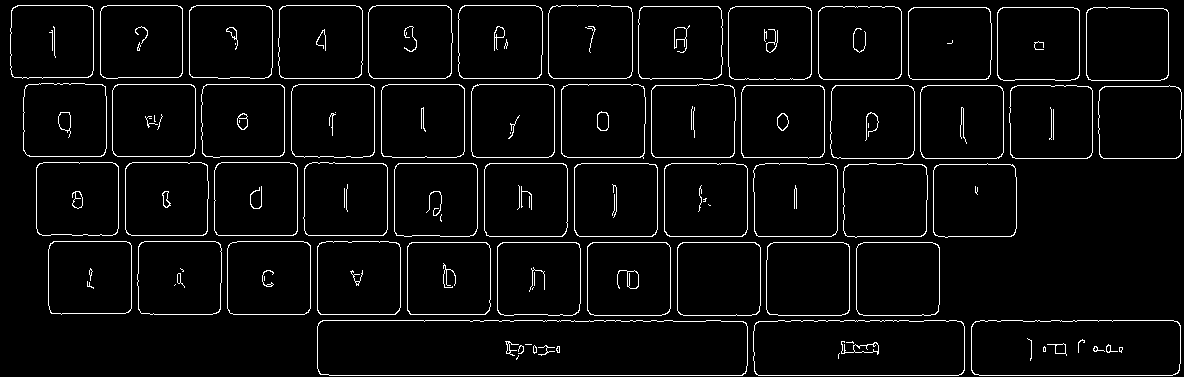
\includegraphics[width=1\textwidth]{img/algorithms/canny-binary.png}
    \vspace{-15pt}
    \caption{Canny detector creates a binary image with discovered edges.}
    \label{algorithms-canny-binary}
\end{figure}

\begin{figure}[hbt]
    \vspace{-9pt}
    \centering
    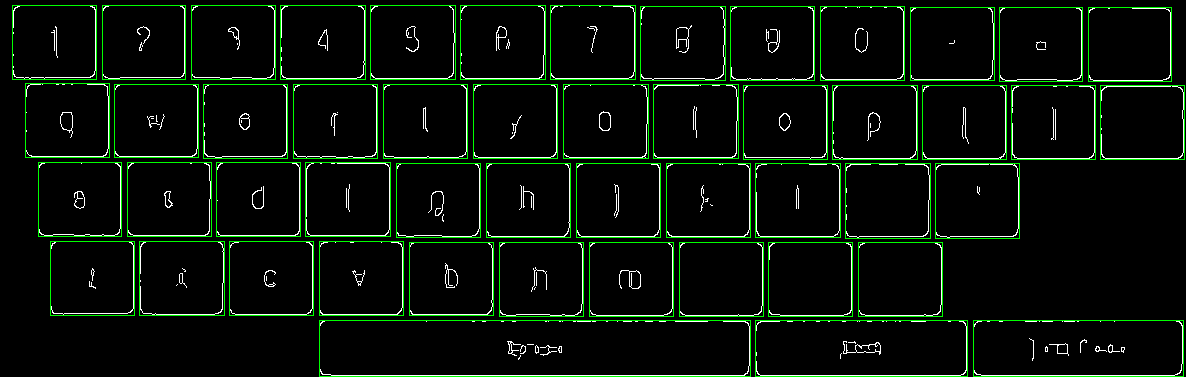
\includegraphics[width=1\textwidth]{img/algorithms/canny-binary-bboxes.png}
    \vspace{-15pt}
    \caption{Contours and their bounding boxes can be computed from the binary image.}
    \label{algorithms-canny-binary-bboxes}
\end{figure}

\begin{figure}[hbt]
    \vspace{-9pt}
    \centering
    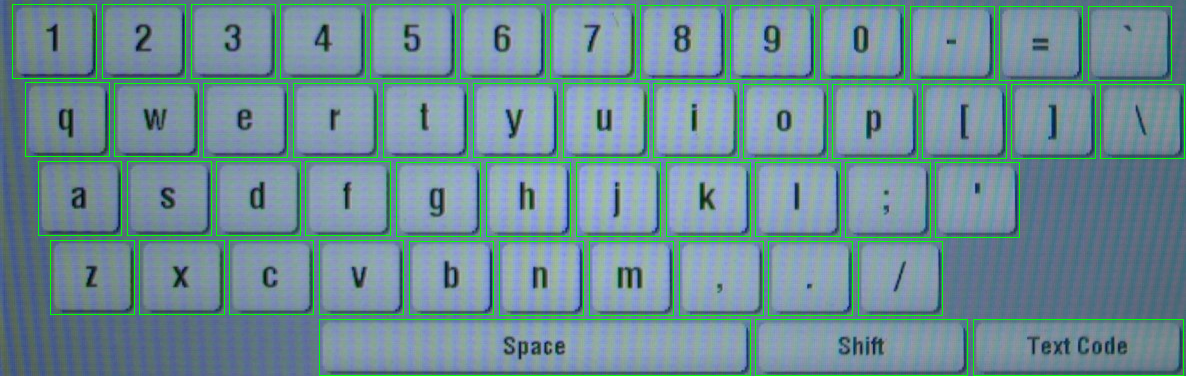
\includegraphics[width=1\textwidth]{img/algorithms/canny-result-bboxes.png}
    \vspace{-15pt}
    \caption{Canny algorithm is capable of detecting key regions on a keyboard.}
    \label{algorithms-canny-result-bboxes}
\end{figure}

\subsection{Thresholding}
\label{algorithms-classical-thresholding}
Thresholding is a method which converts a polychromatic image to a binary one (\hbox{usually} black-and-white). To obtain pixel intensities, the image is typically converted to~grayscale representation. Then a~\hbox{threshold} is chosen and pixels with~intensities above this \hbox{threshold} are set to~one value (white) and the ones below to~another (black). The computation is described by~formula~\ref{thresholding-binary-formula}, where \(I(x, y)\) is pixel intensity on~position \([x, y]\), \(T\) is a threshold and \(G(x, y)\) is the resulting pixel value.

\begin{equation}
  \label{thresholding-binary-formula}
  G(x, y) = \begin{dcases}
 255 & \text{if}\hspace{6pt}I(x, y)\ge\text{T}
 \\
 0 & \text{else}
 \end{dcases}
\end{equation}

However, this method is quite trivial and doesn't work well with~images with different light conditions~\cite{opencv-library}. In~such cases, a different approach such~as adaptive thresholding should be used which computes the threshold from~the neighborhood of~the given pixel. Figure~\ref{algorithms-thresholding-local-global} shows the different results from~global and local thresholding.

\begin{figure}[hbt]
	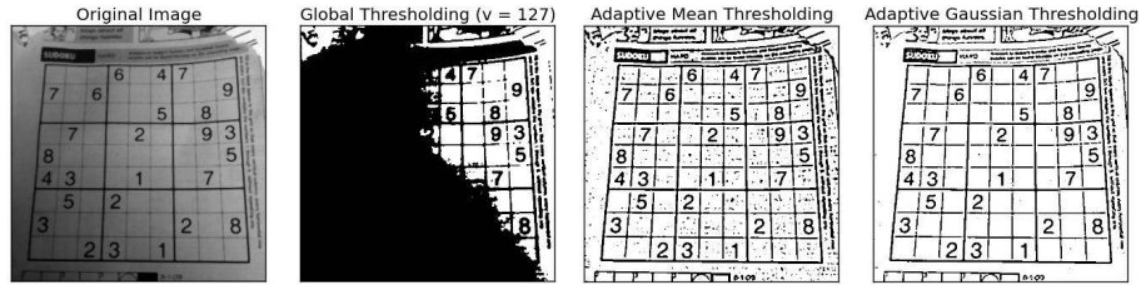
\includegraphics[width=1\textwidth]{img/algorithms/thresholding-local-global.png}
	\caption{Difference between global and adaptive local thresholding (adapted from \cite{opencv-library})}
	\label{algorithms-thresholding-local-global}
\end{figure}

Another popular thresholding method is Otsu's binarization. It is effective and does not require a threshold specification. This method computes probabilities of~pixel intensity values and constructs a histogram. The histogram usually contains~2 major peaks (classes), which represent background and foreground~\cite{opencv-library}. By~iterating over all possible threshold values within the intensity range, the algorithm selects a threshold with~minimum \hbox{intra-class} variance~\cite{otsu-binarization}. Following figure~\ref{algorithms-thresholding-otsu} depicts a~result of~Otsu's thresholding.

\begin{figure}[hbt]
	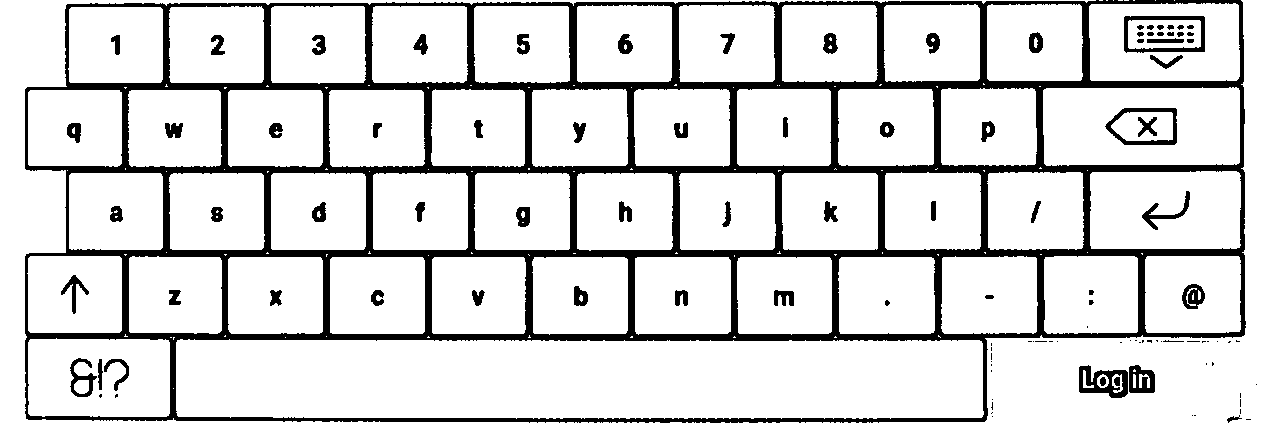
\includegraphics[width=1\textwidth]{img/algorithms/thresholding-otsu.png}
	\caption{Keyboard keys can be detected using Otsu's binarization and bounding boxes acquired by contours computation same as in Canny detector approach \ref{algorithms-classical-canny}.}
	\label{algorithms-thresholding-otsu}
\end{figure}

\section{Neural networks}
\label{algorithms-nn}
Since the success of~AlexNet in~the ILSVRC competition in~2012, convolutional neural networks have become the backbone of~computer vision. There exist many sub-domains of computer vision such as classification, segmentation or image restoration and new ones emerge every day. This section takes a closer look at~object detection sub-domain. The~main problem in~object detection is the localization of the target objects. The objects can be anywhere and by~using classification, a sliding window would have to be used which would classify the object in~it or not. The issue with~this approach is the variability in~the size of~the objects and the number of~classifications necessary. Therefore, new algorithms had to be devised and the next sections describe the most iconic ones.

\subsection{R-CNN}
\label{algorithms-nn-rcnn}
To solve the issue of~a large amount of~sliding window positions for~classification, R-CNN selects only~2000 region proposals using Selective Search algorithm~\cite{selective-search} which can be summed up~to~3 phases~\cite{r-cnn-medium}:

\begin{enumerate}[topsep=0pt,itemsep=-1.5pt,partopsep=6pt]
    \item Generate candidate regions using segmentation.
    \item Merge similar regions using a greedy algorithm.
    \item Create final region proposals.
\end{enumerate}

Once the regions are obtained, each of~them goes into~a ConvNet~\cite{r-cnn-cnn} which extracts \hbox{a 4096-long} feature vector~\cite{r-cnn}. This vector is then classified by the SVM~\cite{svm} algorithm. Apart from the actual detection, 4~offset values are predicted to~improve the bounding box precision (e.g.~part of~the object may be cut, so to~correct it)~\cite{stanford-object-detection-lecture}. Figure~\ref{algorithms-rcnn} demonstrates the whole detection process.

\begin{figure}[hbt]
    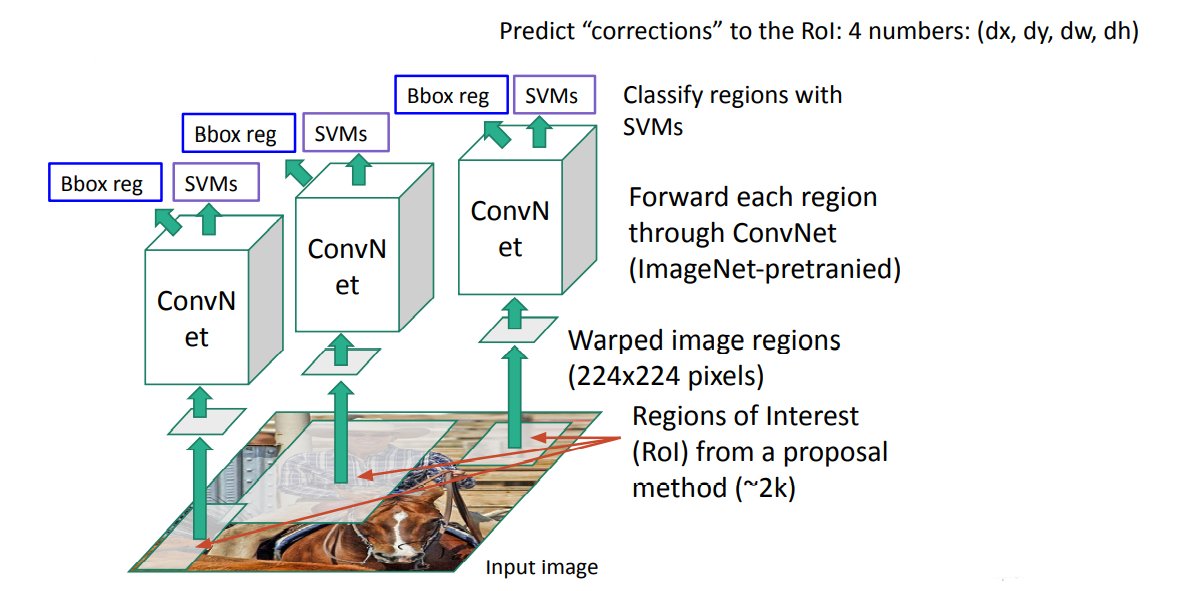
\includegraphics[width=1\textwidth]{img/algorithms/rcnn.png}
    \caption{Object detection process used by R-CNN (adapted from~\cite{stanford-object-detection-lecture})}
    \label{algorithms-rcnn}
\end{figure}

R-CNN achieved remarkable accuracy for~its time and significantly contributed to~the development of~specialized architectures for~object detection. For~instance, on~PASCAL VOC~2012 it improved the accuracy by~30~\% in~comparison to~the best previous result~\cite{r-cnn}.

\subsection{Fast R-CNN}
\label{algorithms-nn-fast-rcnn}
In~spite of~great object detection accuracy, R-CNN is very slow and computationally \hbox{expensive}. Therefore, the author of~the R-CNN tackles the drawbacks in~a new paper~\cite{fast-rcnn}. There are several issues he wanted to~solve:

\begin{enumerate}[topsep=0pt,itemsep=-1.5pt,partopsep=6pt]
    \item \emph{Multi-stage pipeline training} - ConvNet, SVM and bounding box regressors are trained separately.
    \item \emph{Expensive training} - It takes time to~classify~2000 region proposals per~image and space to~store features for~each of~them for~both SVM and bounding box regressors.
    \item \emph{Slow detection} - Features must be extracted for~each region proposal, which means running ConvNet forward pass, and there is no computation sharing.
\end{enumerate}

To~improve the detection speed, features are no longer extracted from~the regions, but instead, the whole image is processed by~the ConvNet. By~doing that, the feature extraction is run only once and the whole image feature map is obtained. An~ROI pooling layer is then used to create a feature vector for~each region proposal. ROI is a window of~rectangular shape which is divided into sub-windows and standard max-pooling is performed on~each of~them~\cite{fast-rcnn}. It is based on~the spatial pyramid pooling layer in~SPPnets~\cite{sppnet} and the same size output is ensured for~the subsequent fully-connected layers as~is depicted in~figure~\ref{algorithms-fast-rcnn-roi}. After~that, the softmax loss function is used to~predict the object class and a bounding box regressor the offset. Due to~2~output layers and single-stage training goal, a multi-task loss is introduced which combines both layers' losses and hence classification and bounding box regression can be trained together~\cite{fast-rcnn}. Full Fast R-CNN architecture is shown in~figure~\ref{algorithms-fast-rcnn}.

\begin{figure}[hbt]
    \centering
    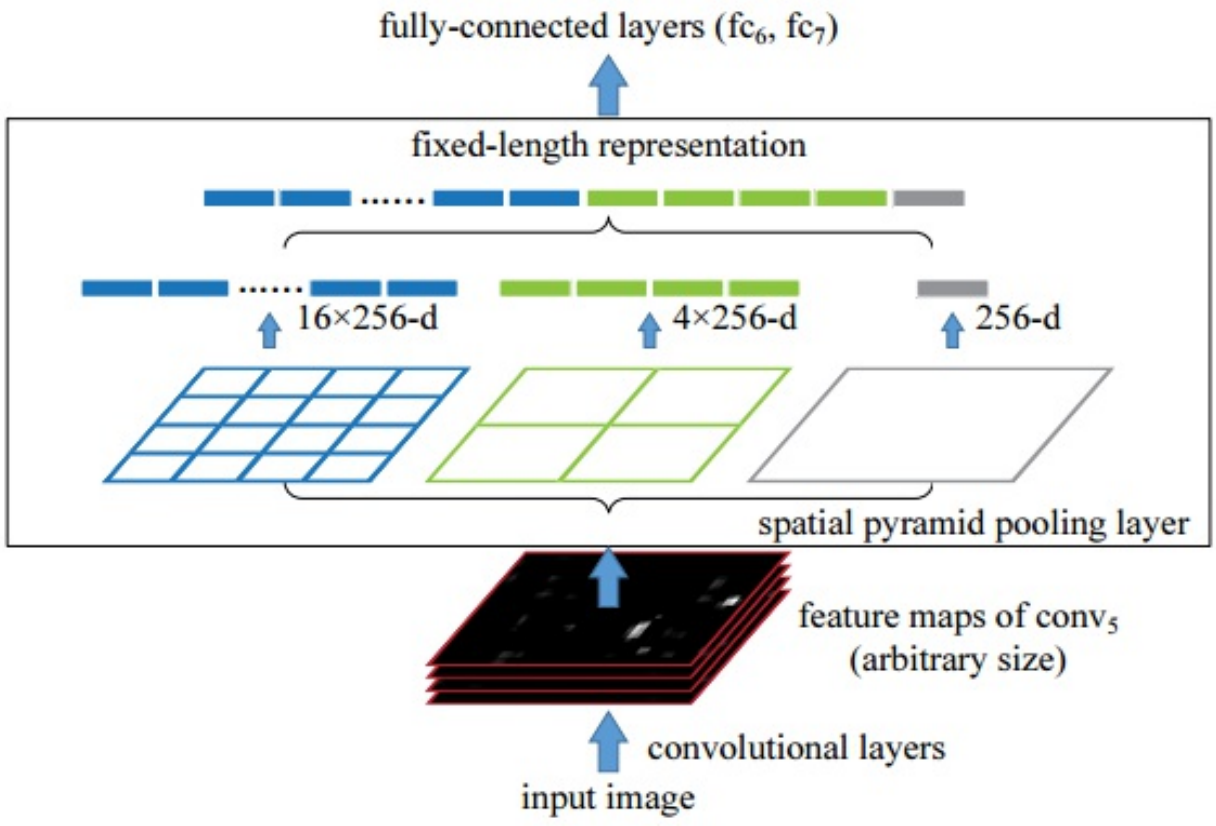
\includegraphics[width=0.8\textwidth]{img/algorithms/fast-rcnn-roi.png}
    \caption{ROI pooling layer in Fast R-CNN (taken from~\cite{hands-on-cnn})}
    \label{algorithms-fast-rcnn-roi}
\end{figure}

\begin{figure}[hbt]
    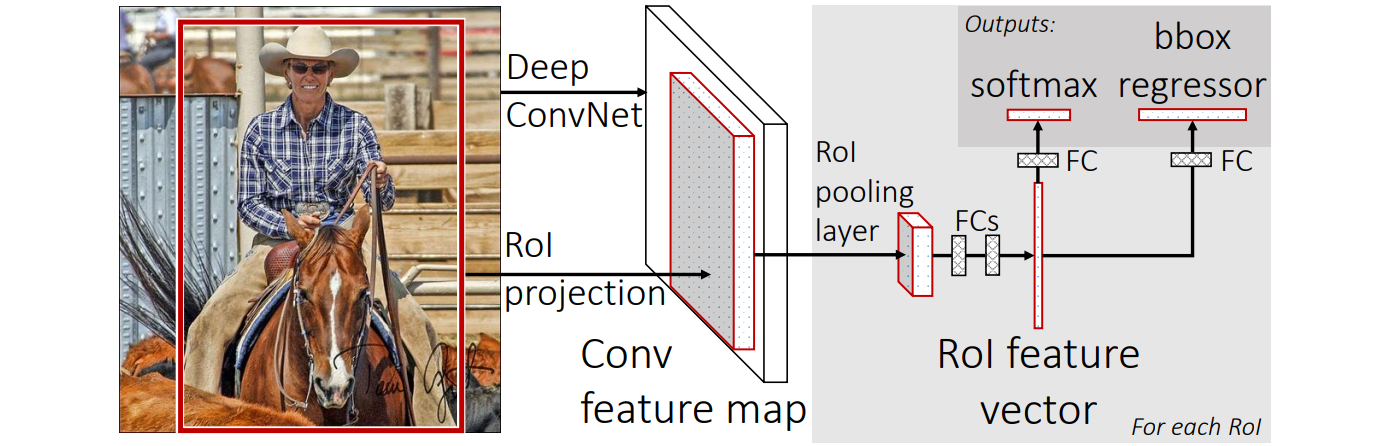
\includegraphics[width=1\textwidth]{img/algorithms/fast-rcnn.png}
    \caption{In Fast R-CNN, a feature map is extracted from~the input image and converted to~a feature vector by~the ROI layer. The softmax then makes the classification and the bounding box regressor finds the offset (taken from~\cite{fast-rcnn}).}
    \label{algorithms-fast-rcnn}
\end{figure}

Fast R-CNN managed to~fix all of the pin-pointed drawbacks. The training became single-stage which can update all layers at~once and there is no need to~store features on~disk anymore~\cite{fast-rcnn}. In~addition, detection is much faster and even more accurate~\cite{fast-rcnn}. Compared to~the R-CNN, training time got reduced almost 10 times and test time 23~times including the region proposals and nearly 147 times excluding them~\cite{stanford-object-detection-lecture}.

\subsection{Faster R-CNN}
\label{algorithms-nn-faster-rcnn}
R-CNN and Fast R-CNN share a common problem which is the use of~Selective Search algorithm for~region proposals. Selective Search on~its own is rather popular and effective, but in~comparison with~neural networks, it is slower by~a~margin as it takes around~2~seconds per~image to~find the regions~\cite{faster-rcnn}. It doesn't matter much to~R-CNN since it is quite slow and the performance hit is not so noticeable. However, Fast~R-CNN without the region proposals achieves almost real-time rates and the 2-second hit increases computation 7~times~\cite{stanford-object-detection-lecture}. Faster~R-CNN aims at replacing Selective Search with Region Proposal Network (RPN) as~shown in~figure~\ref{algorithms-faster-rcnn}.

\begin{figure}[hbt]
    \centering
    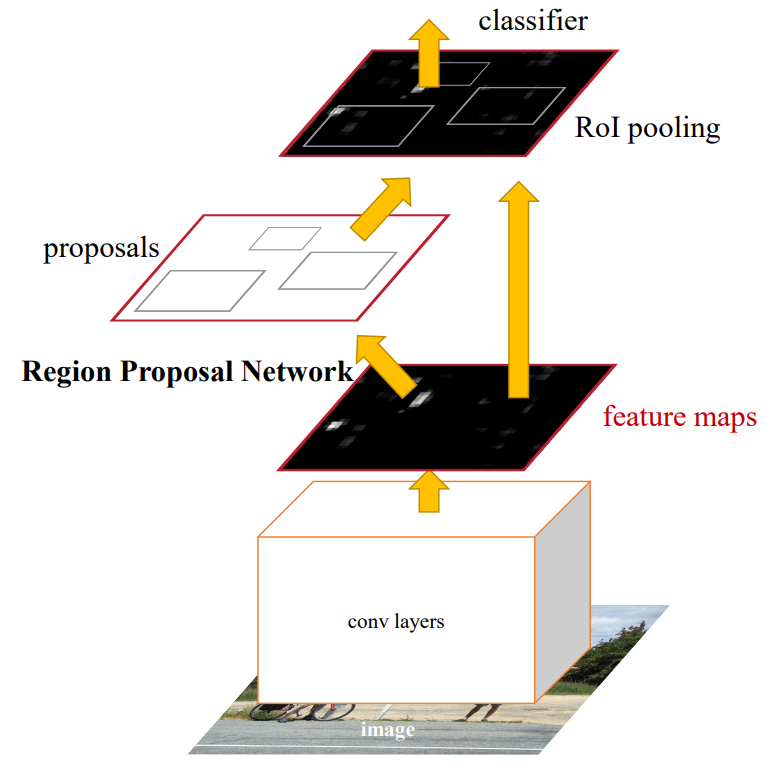
\includegraphics[width=0.6\textwidth]{img/algorithms/faster-rcnn.png}
    \caption{Faster R-CNN is essentially Fast R-CNN with~a neural network in~place of Selective Search (taken from~\cite{faster-rcnn}).}
    \label{algorithms-faster-rcnn}
\end{figure}

To understand better how RPN works and how it is included in~the model architecture, the \hbox{original} paper~\cite{faster-rcnn} describes it quite clearly. Still, I will provide a short summary. As~the idea is to train the whole model together, RPN shares the convolutional layers with the \hbox{Fast R-CNN} and works on~the output of~the last convolutional layer, the feature map. It~passes a \hbox{rectangular} sliding window through the map and generates several region proposals for~each window. The proposals are then parameterized relative to reference boxes called anchors. The anchors lie at~the center of~the sliding window and have different scales, so~the detection is \hbox{size-indifferent}. A~feature vector is extracted for~each proposal and a sibling \hbox{two-layer} network predicts the region coordinates and an objectness score defining, how sure it is that an object is in~the region. This is visualised in~figure~\ref{algorithms-faster-rcnn-rpn}.

\begin{figure}[hbt]
    \centering
    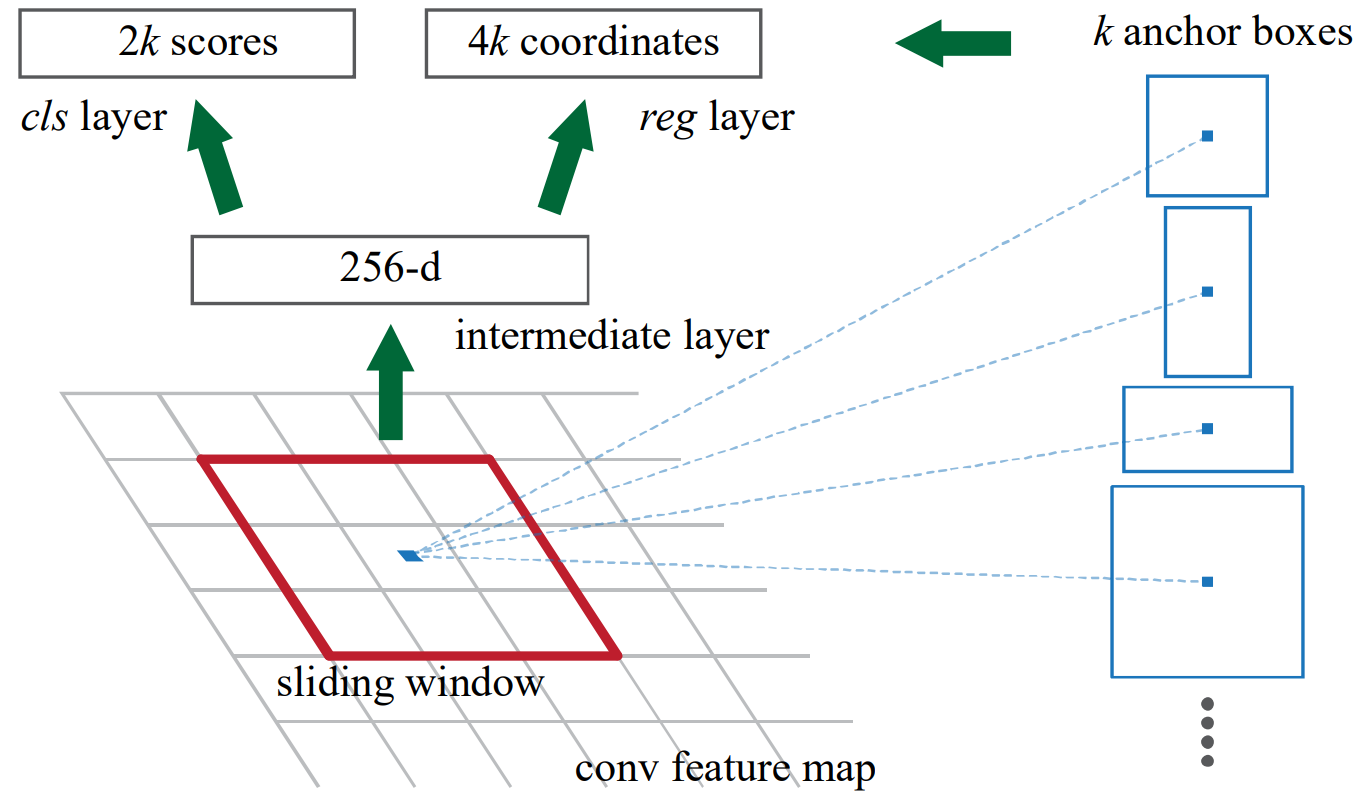
\includegraphics[width=0.7\textwidth]{img/algorithms/faster-rcnn-rpn.png}
    \caption{Region extraction in Region Proposal Network (taken from~\cite{faster-rcnn})}
    \label{algorithms-faster-rcnn-rpn}
\end{figure}

During the training, the intersection-over-union of~anchors and \hbox{ground-truth} boxes is computed. If an anchor is eighter the highest scoring or scores over~0.7~with any \hbox{ground-truth} box, it is assigned a positive label for~being an object. Having removed the Selection Search algorithm, it takes only~0.2 seconds to~process an image which makes it a real-time object detector and~11 times faster than the Fast R-CNN~\cite{stanford-object-detection-lecture}.

\subsection{YOLO}
\label{algorithms-nn-yolo}
YOLO (You only look once) brought a novel approach to~the object detection field. As~the authors of this algorithm~\cite{yolo} claim, the detection systems at~that time reused classifiers for the evaluation of certain windows in~an image. In~spite of~having methods for~selecting such windows, the R-CNN family is no different. What is more, the whole process is a pipeline of~several actions and all the R-CNN algorithms need to~look at~the image twice, once for~region proposal generation, and once for~object detection of~the proposals. YOLO, on~the other hand, needs only one look and is capable of~making the classification and bounding box regression simultaneously. Instead of~a single region, it sees the whole image which allows it to encode context information and as a result, it makes significantly fewer background errors than R-CNN based algorithms. Owing to all of~this, YOLO is extremely fast. Nevertheless, it lacked in~accuracy in~comparison with~the state-of-the-art approaches at~the time~\cite{yolo}.

The process of~finding the bounding boxes is described by~the paper~\cite{yolo} as~follows. The image is divided into a \(S\) x \(S\) grid which portrays figure~\ref{algorithms-yolo-grid} and a grid cell, which is a center of~an object, is responsible for~its detection. Each grid cell predicts \(B\) bounding boxes and their confidence scores, which reflects the intersection-over-uniou (IoU) with the ground-truth. To~predict a bounding box, the neural network uses features from the entire image. However, excess bounding boxes can be produced by neighboring grid cells for the same object. This is solved by non-maximal suppression. Apart from~the object location, the grid cell also predicts the object class probabilities.

\begin{figure}[hbt]
    \centering
    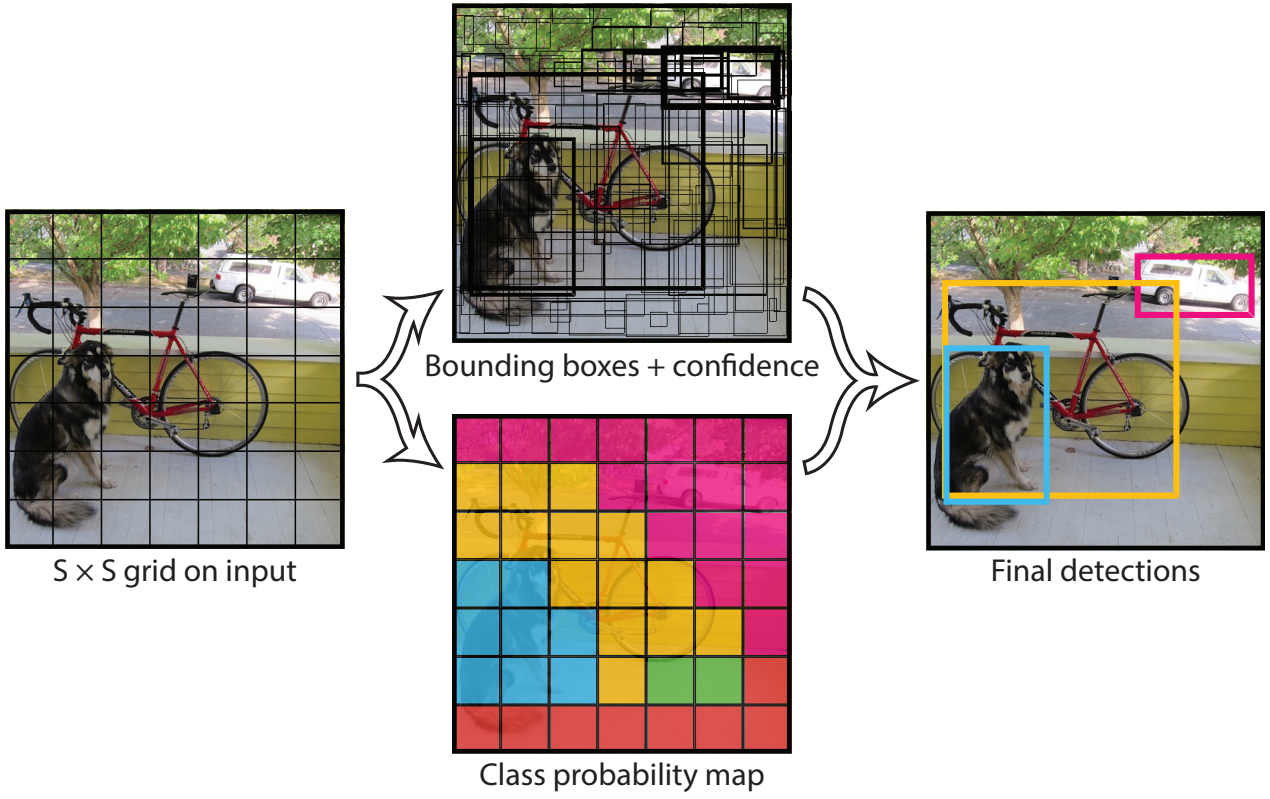
\includegraphics[width=0.9\textwidth]{img/algorithms/yolo-grid.png}
    \caption{YOLO uses a grid to~predict bounding boxes and object classes (taken from~\cite{yolo}).}
    \label{algorithms-yolo-grid}
\end{figure}

The architecture of~YOLO is based upon~the GoogLeNet~\cite{googlenet} with~the modification of~using 1x1 reduction layers followed by 3x3 convolutional layers instead of~GoogLeNet's inception modules~\cite{yolo}. Consequently, the network has~24 convolutional layers followed by~2~fully connected layers as~figure~\ref{algorithms-yolo-architecture} shows. The features are extracted by~the initial convolutional layers and the fully connected layers then produce the bounding boxes and class predictions~\cite{yolo}.

During the training, leaky ReLU activations are used in~the hidden layers and normal ReLU in~the final layer~\cite{yolo}. For~optimization, sum-squared error is utilized for~its simplicity, although it weights classification and localization errors equally, which is a downside~\cite{yolo}. The loss function is multi-part and consists of~5 terms. These terms are for~the object's center coordinates, bounding box dimensions, object class, a class in~case of~the object's absence and probabilities of~finding the same object respectively~\cite{yolo-evolution}.

\begin{figure}[hbt]
    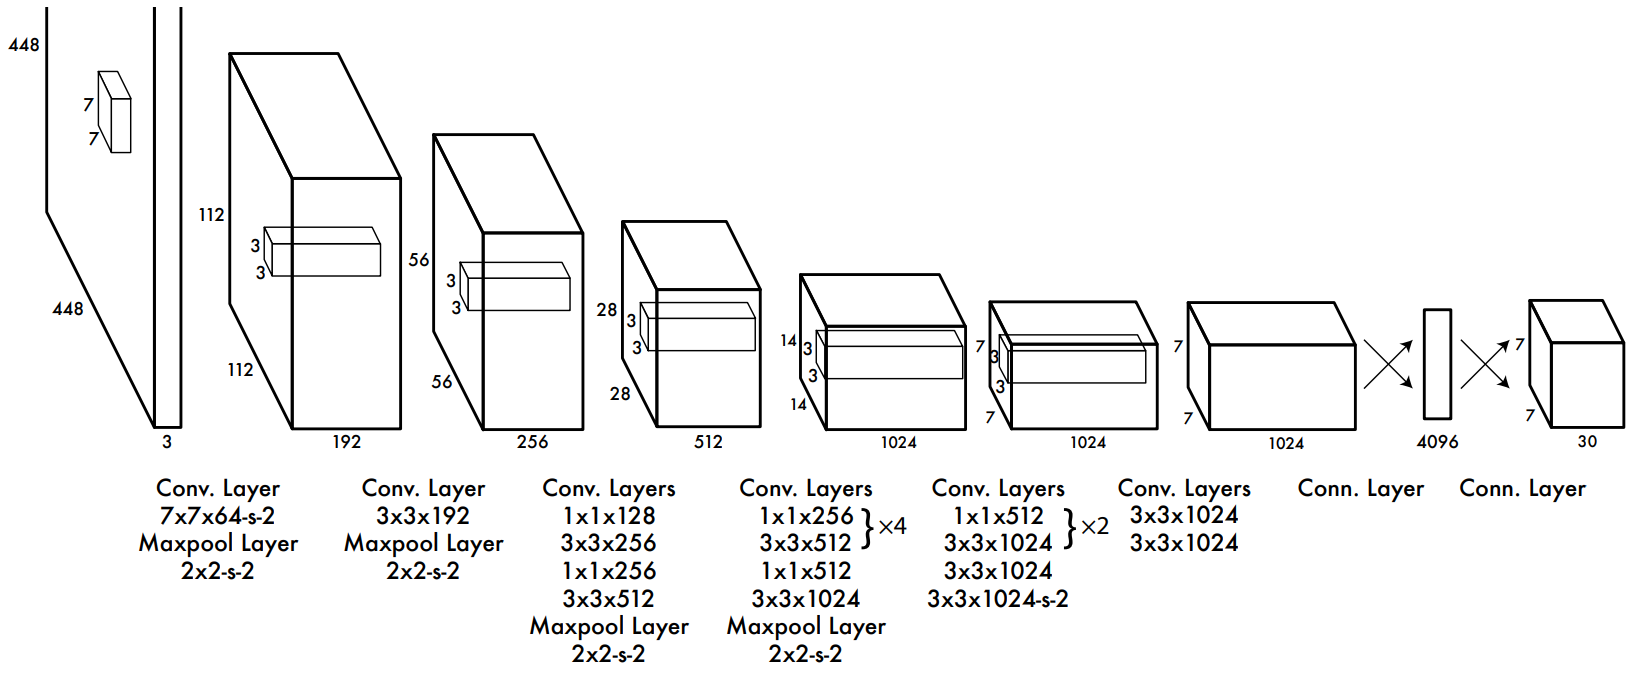
\includegraphics[width=1\textwidth]{img/algorithms/yolo-architecture.png}
    \caption{Architecture of YOLO network (taken from~\cite{yolo})}
    \label{algorithms-yolo-architecture}
\end{figure}

However, not even the novel approach of~YOLO is without limitations and the authors are well aware of them and mention them in the paper~\cite{yolo} as well. As each grid cell predicts only a few bounding boxes and a single class, it imposes a spatial constraint which causes difficulties in prediction of small objects like flocks of birds. Furthermore, it struggles with generalization of unusual aspect ratios. It has problems with localization errors. Still, it worked extremely well among other real-time object detectors and new versions fixing those issues have been being developed due to its popularity ever since.

\subsubsection{YOLOv2}

YOLOv2~\cite{yolov2} brought several improvements. These are very well summarized by~article~\cite{yolo-evolution} from~which the most important ones are listed:

\begin{itemize}[topsep=0pt,itemsep=-1.5pt,partopsep=6pt]
    \item Batch normalization is used instead of~dropout layers.
    \item Resolution detail is increased by the removal of~a max-pool layer, which leads to~better accuracy.
    \item Location is predicted with~respect to~a grid cell instead of~an anchor box. This means better stabilization during the training.
    \item Feature map is more fine-grained (13x13).
    \item Fully-connected layers are replaced with~convolutional ones, which allows for~multi-scale training.
    \item VGG-16 backbone is replaced by~Darknet-19.
    \item Hierarchical classification is introduced. This allows for~assigning several classes (e.g.~dog and their breed) to objects whereas before they were mutually exclusive.
\end{itemize}

As~a result, YOLOv2 improved especially in~accuracy, recognition of~smaller objects, but also in~speed. It became state-of-the-art in~both speed and accuracy without any obvious limitations.

\subsubsection{YOLOv3}
YOLOv3 focuses mainly on~improving speed and accuracy, rather than fixing some known issues as the name of~paper~\cite{yolov3} \say{YOLOv3: An Incremental Improvement} also suggests. This paper introduces the following changes. The objectness score is calculated using logistic regression and the sigmoid function is used to~predict the bounding box center. In~class prediction, a switch to~cross-entropy from~the sum-squared error was made. Moreover, a~new deeper backbone Darknet-53 is used.

\subsubsection{YOLOv4}
This version of YOLO is very important because the creator of~YOLO, Joseph Redmon, retired from~computer vision and new researchers continued with~YOLO advancements. They came to the conclusion, that a general object detector consists of~several parts, which are input, backbone, neck and head~\cite{yolov4}. They decided to map YOLO into this decomposition as~figure~\ref{yolov4-decomposition} depicts.

\begin{figure}[hbt]
    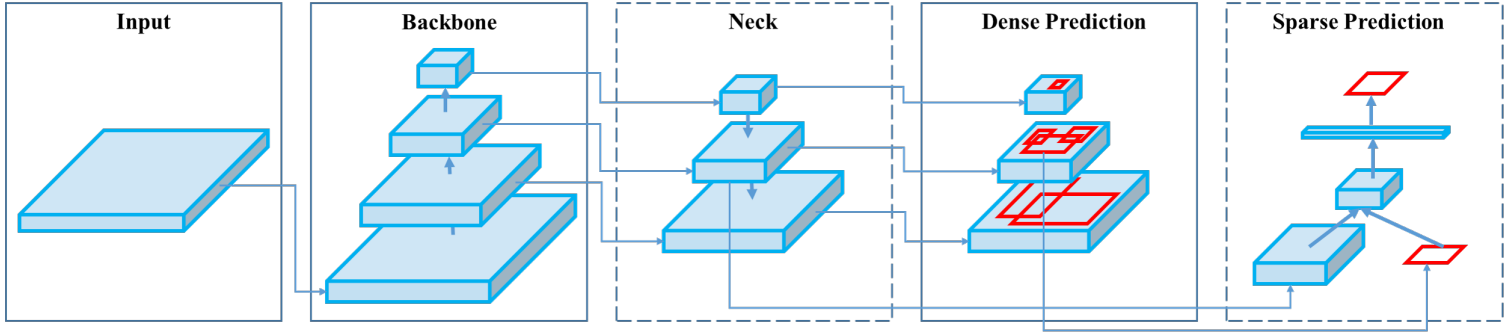
\includegraphics[width=1\textwidth]{img/algorithms/yolov4-decomposition.png}
    \caption{In~YOLOv4, input is the input image. Backbone is the feature extraction network which was updated from~Darknet53 in~YOLOv3 to~CSPDarknet53. The neck is supposed to~be the region selection part, the spatial pyramid pooling, which underwent subtle modification in~YOLOv4 to improve accuracy. Lastly, the head takes care of~the class and location prediction which in~this figure are the dense and sparse prediction blocks (adapted from~\cite{yolov4}).}
    \label{yolov4-decomposition}
\end{figure}

The new authors also introduce bag of~freebies and bag of~specials. Bag of~freebies are methods that improve performance without increasing inference time in~production~\cite{yolov4}. They can be viewed as some plugin modules which one can try to~improve a model. There is a huge amount of them and they are usually normalization or regularization methods, data augmentation, data imbalance etc. From~those that YOLOv4 uses can be named e.g.~Mosaic data augmentation, DropBlock regularization, class label smoothing and many othes~\cite{yolov4}. Concerning the bag of specials, those are post-processing methods which do have a small impact on~inference time but bring a significant accuracy increase. Out~of~these, mish activations, Cross-Stage Partial (CSP) Connection or SPP blocks for instance are applied in~YOLOv4~\cite{yolov4}.

\subsubsection{YOLOv5}
YOLOv5 was developed by~different authors than YOLOv4 and was released just a month after the previous version. Research on~both of~them started relatively at~the same time and was conducted simultaneously. It was named YOLOv5 simply to avoid a collision~\cite{yolo-evolution-thesis}. As~a result, due to the parallel work and application of~the same state-of-the art innovations in~the field, the architectures of~both do not differ much~\cite{yolo-evolution-thesis}. YOLOv4 paper even acknowledges Glenn Jocher, the author of YOLOv5, for~the Mosaic data augmentation~\cite{yolov4}. Consequently, both models perform very similarly, however, YOLOv5 appears to~be a bit faster and YOLOv4 slightly more accurate when more custom configuration is applied~\cite{yolov5-vs-yolov4}. Owing to the naming, timing, lack of~outstanding improvements in~comparison with~the previous version and most importantly no research paper, YOLOv5 was a source of~quite a controversy in~the computer vision community. Nevertheless, it got accepted eventually.

\subsubsection{YOLOv6}
YOLOv6 further advances both speed and accuracy of~YOLO algorithm and beats all other real-time detectors at~the time~\cite{yolov6}. It further improves the backbone which is now named EfficientRep consisting of~RepBlocks~\cite{yolov6}. These RepBlocks also replace the CSP blocks in~the neck~\cite{yolov6}. Main architectural change brings the head, though. Instead of~1~head,~3~heads are used as~figures~\ref{yolov6-architecture} and~\ref{yolov6-head} show.

\begin{figure}[hbt]
    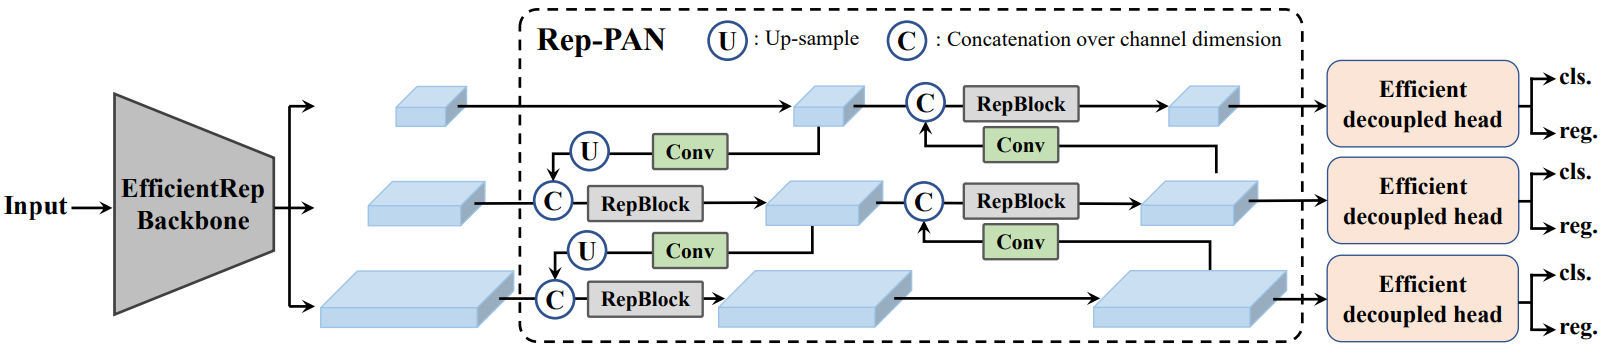
\includegraphics[width=1\textwidth]{img/algorithms/yolov6-architecture.png}
    \caption{In~YOLOv6, neck outputs go to~3 decoupled heads. In~the previous versions, localization and classification heads were coupled, which means that they shared the same features and more computation was needed~\cite{yolov6} (taken from~\cite{yolov6}).}
    \label{yolov6-architecture}
\end{figure}

\begin{figure}[hbt]
    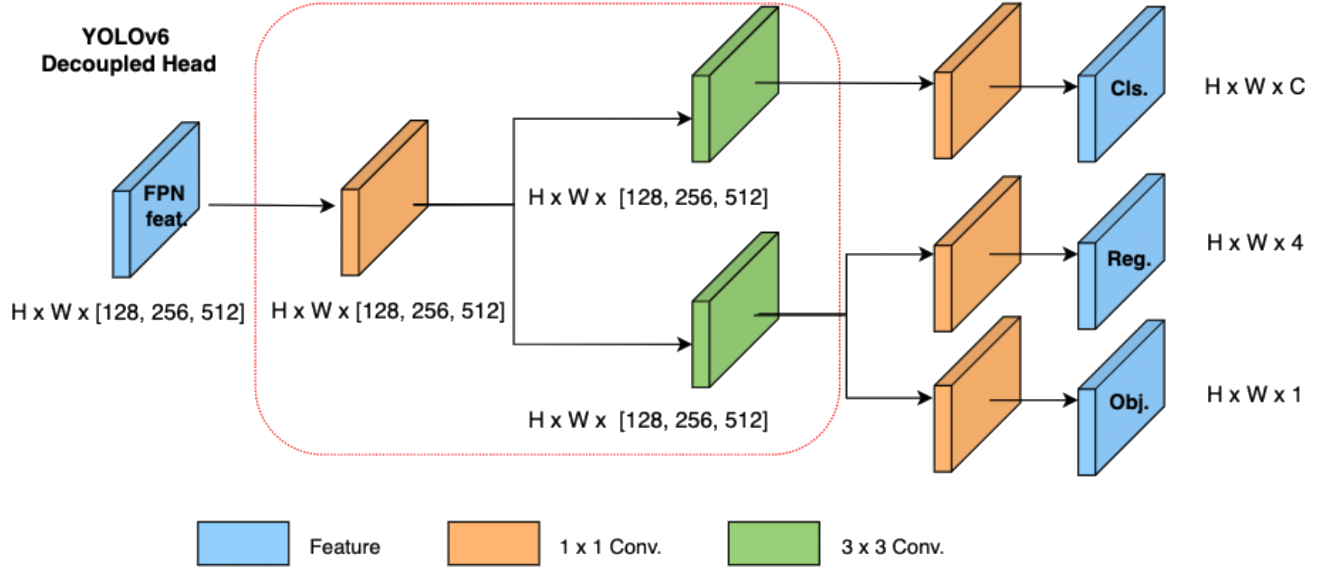
\includegraphics[width=1\textwidth]{img/algorithms/yolov6-head.png}
    \caption{In~a head, 3~loss functions are computed. Cross-entropy for classification and L1 for regression were left the same from~the previous versions. A~new object loss is \hbox{computed}, which aims at~reducing the score of~low-quality bounding boxes but unfortunately does not have many effects~\cite{yolov6} (taken from~\cite{yolov6-roboflow}).}
    \label{yolov6-head}
\end{figure}

\subsubsection{YOLOv7}
Similarly to~YOLOv4 and YOLOv5, the release of~YOLOv6 and YOLOv7 was very close. There are still debates about which one is better but more benchmarks found on~the internet favour the latter. Moreover, the YOLOv7 paper claims better results than YOLOv6 on~the COCO dataset~\cite{yolov7}. According to some~\cite{yolov7-web}, it is even expected of~YOLOv7 to~become the new industry standard. It might also be worth mentioning that YOLOv7 come from the same authors as~YOLOv4. The most important contributions of~YOLOv7 are the following:~\cite{yolov7}

\begin{itemize}[topsep=0pt,itemsep=-1.5pt,partopsep=6pt]
    \item \emph{Extended efficient layer aggregation} -- Efficiency of~the convolutional layers is the key to~the inference speed. Hence, building heavily on~research on~this topic, using group convolution to~increase feature cardinality and combining features of~different groups leads to an improved feature learning process.
    \item \emph{Model scaling for concatenation-based models} -- While other models usually scale the width or~depth of the network, YOLOv7 scales them together which keeps the architecture optimal for~different sizes.
    \item \emph{Planned re-parameterized convolution} -- Re-parameterization means averaging weights to~create a more robust model. Which network modules to~re-parameterize is determined by~gradient flow propagation paths.
    \item \emph{Auxiliary heads} -- Network heads making the prediction are quite far. Other heads placed in~the middle of~the network help with the training.
\end{itemize}

\subsubsection{Others}
Apart from the main versions of~YOLO, other YOLO mini-series such as~YOLOX, YOLOR or PP-YOLO have emerged. They (and their newer versions) usually build upon a~current YOLO version and improve it in~certain ways. YOLOX for example removes the anchor boxes and YOLOR combines explicit and implicit knowledge to~perform several tasks. However, covering all these YOLO offspring is out of~scope of~this thesis.

\subsection{Single Shot Detector}
\label{algorithms-nn-ssd}
Similarly to~YOLO, Single Shot Detector (SSD) needs only one look at~an image to process it. At~the time, it outperformed both YOLOv1 and R-CNN-based algorithms in~speed and accuracy alike~\cite{ssd-paper}. Same as~the original YOLO, it uses the VGG-16 net as~a backbone on~which it builds additional convolutional layers as~depicted in~figure~\ref{ssd-architecture}.

\begin{figure}[hbt]
    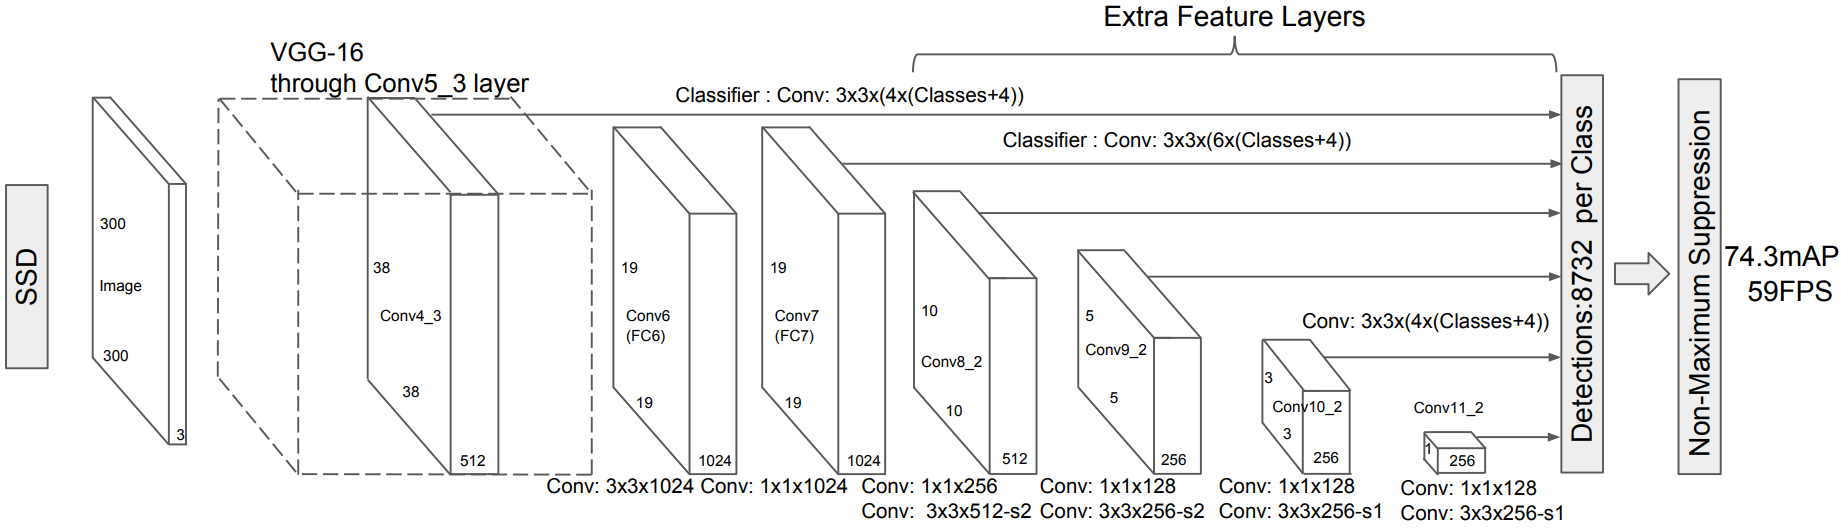
\includegraphics[width=1\textwidth]{img/algorithms/ssd-architecture.png}
    \caption{SSD architecture consists of~VGG-16 backbone followed by~additional convolutional layers. The classifiers in~extra feature layers use 3x3 convolutions for~\emph{k} (4~or~6) bounding boxes for~\emph{N} classes~+~4 offsets. Non-maximum suppression is used at~the end to handle intersecting bounding boxes (adapted from~\cite{ssd-paper}).}
    \label{ssd-architecture}
\end{figure}

SSD can be also called Single Shot MultiBox Detector because it uses multiple boxes for~localization. The original paper~\cite{ssd-paper} describes the bounding box selection as~follows. The added convolutional layers scale down so that multi-scale prediction can be done. Each of~them contributes to~the result with~its set of~detections. A~certain feature map has size \(m\)~x~\(n\) which is a number of~locations (feature map cells). A~default set of~bounding boxes is associated with~each location as~shown in~figure~\ref{ssd-multibox}.

\begin{figure}[hbt]
    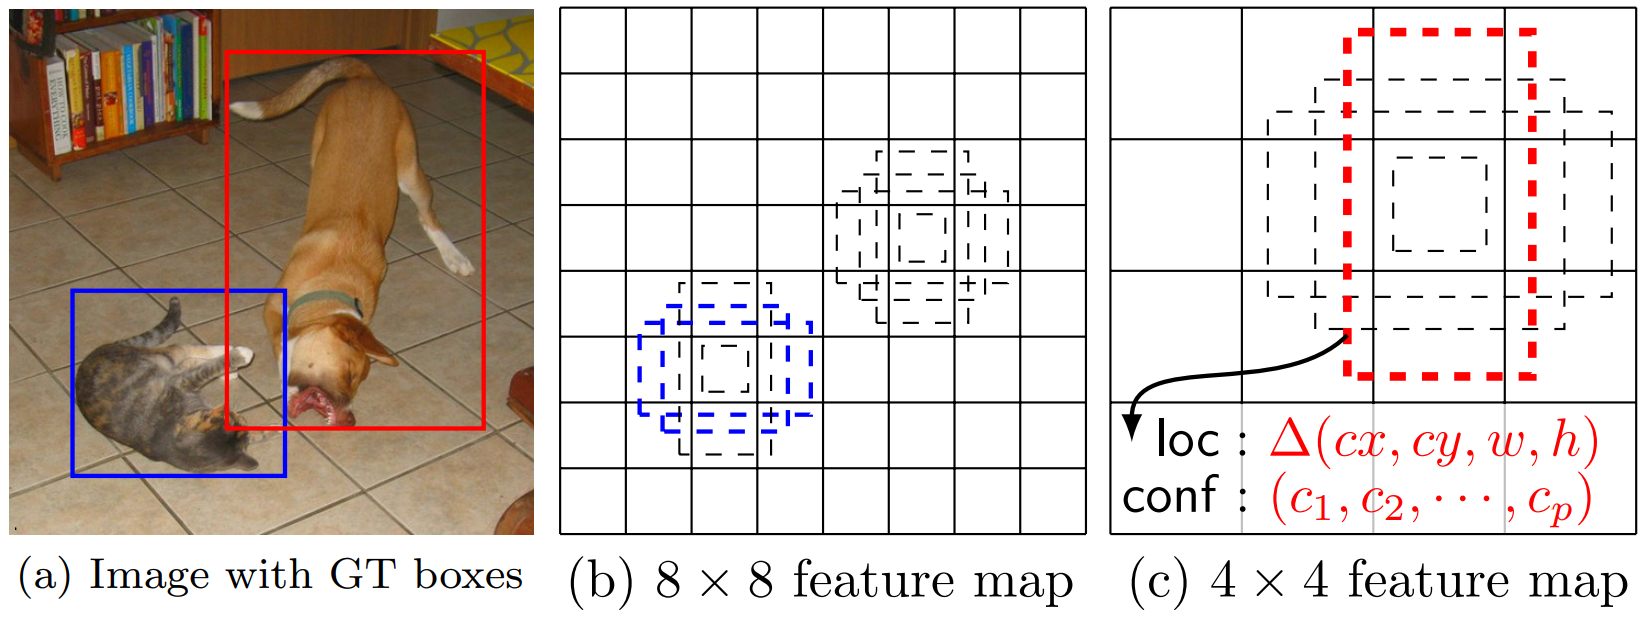
\includegraphics[width=1\textwidth]{img/algorithms/ssd-multibox.png}
    \caption{Each feature map cell has \emph{k} (usually 4~or~6) default bounding boxes. The idea is that a person, for~instance, would need a vertical box whereas a car would need a horizontal one (taken from~\cite{ssd-paper}).}    
    \label{ssd-multibox}
\end{figure}

Then we can easily get to~the~8732 detections from~figure~\ref{ssd-architecture} like this:

\begin{itemize}[topsep=0pt,itemsep=-1.5pt,partopsep=6pt]
    \item Conv4\_3: 38 x 38 x 4 = 5776
    \item Conv7: 19 x 19 x 6 = 2166
    \item Conv8\_2: 10 x 10 x 6 = 600
    \item Conv9\_2: 5 x 5 x 6 = 150
    \item Conv10\_2: 3 x 3 x 4 = 36
    \item Conv11\_2: 1 x 1 x 4 = 4
\end{itemize}

For~an image of size 300x300 is done \(5776 + 2166 + 600 + 150 + 36 + 4 = 8732\) detections. In~comparison with YOLOv1 which makes only~98 detections for~a 448x448 image, it is an extreme improvement and the main source of~the accuracy boost~\cite{ssd-paper}.

Concerning the loss function, while YOLOv1 used~5 terms based on~the sum of~squares, SSD uses only two-term loss~\ref{ssd-loss}~\cite{ssd-paper}:

\begin{equation}
  \label{ssd-loss}
  L(x, c, l, g) = \frac{1}{N}(L_{conf}(x, c) + \alpha L_{loc}(x, l, g))
\end{equation}

\(L_{conf}\) is the softmax loss function for~class prediction which takes \(x \in \{1, 0\}\) as~an indicator if the box matches the ground-truth and \emph{c} as the class confidence. \(L_{loc}\) is the Smooth L1 localization loss and \(l, g\) the predicted and ground-truth boxes respectively. \emph{N}~denotes the number of~matched bounding boxes.

Then there is the question of~how the default bounding boxes are determined. Suppose there are \emph{m} feature layers, the scale for~each layer's bounding boxes is determined by~the following equation~\ref{ssd-scale}~\cite{ssd-paper}:

\begin{equation}
  \label{ssd-scale}
  s_k = s_{min} + \frac{s_{max} - s_{min}}{m - 1} (k - 1), \hspace{0.5cm} k \in \langle1, m\rangle
\end{equation}

In~this equation \(s_{min} = 0.2\) and \(s_{max} = 0.9\), which makes the scale of~the lowest layer~0.2, the highest layer~0.9 and other layers regularly spaced. Default boxes' aspect ratios are then \(a_r \in \{1, 2, 3, \frac{1}{2}, \frac{1}{3}\}\) (excluding 3 and \(\frac{1}{3}\) when only 4 boxes are used) and a box size is computed as~\(width_k^a = s_k \sqrt{a_r}\) and \(height_k^a = \frac{s_k}{\sqrt{a_r}}\)~\cite{ssd-paper}.

The large amount of~generated bounding boxes comes with a price, though. Most of~the boxes are naturally negatives which creates an imbalance between positive and negative training samples~\cite{ssd-paper}. To~solve this issue, the hard negative mining technique is used. To~achieve more stable training and faster optimization, only the negatives with the highest confidence score are picked. In~addition to~this, to~improve the training and to~make the model more robust, data augmentation is heavily employed.

In~spite of~achieving better results than any other object detector at~the time, no further advancements or newer versions of~SSD seem to~be around. While it undoubtedly influenced many object detection architectures, SSD itself got soon dethroned as~the state-of-the-art by newer versions of~YOLO. Nevertheless, it can still be seen in~many object detection applications amongst~which the Amazon's keyboard detection~\cite{amazon-paper} can be counted.
  \chapter{Dataset}
\label{dataset}
After a thorough internet search, no dataset suitable for~keyboard let alone keys detection could be found at~the time of~writing this thesis. The Amazon research team struggled with the same issue and was forced to~create its own dataset~\cite{amazon-paper}. Nonetheless, not even their dataset seems to~be published. Consequently, to achieve the goal of this work, I was compelled to create my own datasets for~keyboard detection, keys detection and post-processing corrections. The contribution of my datasets is not only to~keyboard typing automation tasks such as~mine but also to others like single-character recognition for~instance.

\section{Keyboards}
\label{dataset-keyboards}
As~it turned out, collecting a sufficient amount of~keyboards was not an easy task. The primary source of~keyboard images became Google and Bing search engines followed by~the Pinterest platform. The main issue with the internet keyboard images is their low utility. As~discussed in~section~\ref{introduction-expectation}, the images for~the detection will be \hbox{full-HD} and not distorted nor rotated. Many of~the keyboards found by~the search engines are either of~really low quality, from~a perspective or with~the user's fingers on~them. However, the low-resolution images were still kept as~long as~the characters were readable. Moreover, these keyboards were usually set in~lowercase mode as~most of~them, from my observation, come from android devices where it is the default mode. Uppercase mode keyboards were significantly harder to~find and special characters were particularly difficult to~come by. The~secondary source was my~own mobile phone on~which several keyboard applications with~different designs and key layouts were installed. From these, all keyboard modes were obtained. Other sources were personal devices such as~tablets, e-book readers and smart TVs or company printers on~which AIVA units already operate.

In~the end, 615~keyboard images were gathered. While it might not sound as~much, the Amazon working solution used only over a hundred different keyboard styles for~the keyboard detection~\cite{amazon-paper}, which I significantly surpass. Even for the keys detection, the Amazon researches labelled keys from only~634 images~\cite{amazon-paper}. This is roughly the same as~me and it further proves the difficulty of~obtaining a substantial amount of~keyboards and also that this amount is sufficient for~the task. The keyboards were collected from~various device types (smartphones, tablets, desktop computers, laptops, car infotainments, e-book readers, printers, TVs and pin pads) in~both digital and physical form. From~the original images, only the keyboard regions were kept and placed on~a background in~a manner specified by~section~\ref{dataset-keyboards-generation}. 

To~prepare the dataset for training, it is split into train-validation-test in~a~70:20:10 ratio. Therefore, 429~keyboards are selected for~training, 124 for~validation and 62~for~testing. The training set is further augmented to~20~000~samples, same as done by the Amazon team~\cite{amazon-paper}, using the techniques described in~section~\ref{dataset-keyboards-augmentation}.

\subsection{Dataset generation}
\label{dataset-keyboards-generation}
Placing a keyboard region on~a background comes with the benefit of~no need for~\hbox{manual} object annotation. Exactly one keyboard is placed in~each image and an~annotation JSON file with~the format depicted by~figure~\ref{keyboard-annotation-json} is generated for~each training/validation/testing image set.

\vspace{-6pt}
\begin{figure}[hbt]
    \centering
    \begin{boxedverbatim}
"1.png": [0, 49, 1280, 574],
"2.png": [71, 470, 1017, 692],
"3.png": [237, 179, 1041, 407],
...\end{boxedverbatim}
    \caption{Keyboard annotation file is a JSON dictionary with a filename as~a key and bounding box coordinations in~format [x1, y1, x2, y2] as~a value.}
    \label{keyboard-annotation-json}
\end{figure}

Despite the fact that the object detection input will be a full-HD image, I decided to use HD resolution for~backgrounds. The first and main reason is the size. The resulting dataset would attack 100~GB of~space and both the training and inference would take an unnecessarily long time. Moreover, the detected region can easily be scaled back so that the keyboard region from~the original full-HD image is used later. The second reason is that the Amazon researchers used SSD300 model for~the keyboard detection~\cite{amazon-paper}, so clearly HD image is still more than enough. In~the Amazon paper, they placed the keyboard regions on~random images from the COCO~2017 dataset~\cite{amazon-paper}. Although I was inspired by~this idea due to~the large scale of~scene backgrounds, I found it odd that there are hard edges where the keyboard starts in~an image. In~theory, just being a rectangle of~different color might add a~lot to~the keyboard detection. For~this reason, I decided to use the COCO dataset just for~half of~the images. For~another 40~\%, the average border color of~the keyboard is used as~the background so that the keyboard seemingly blends~in. Hence, the keyboard keys and characters layout become more important. Figure~\ref{keyboard-bg-comparison} shows the difference. Concerning the rest, 5~\% of~keyboards are rendered on~a completely random background color and 5~\% on~a random color gradient.

\vspace{-4pt}
\begin{figure}[tbh]
    \centering
    \subfloat[\centering COCO 2017 image as a background]{{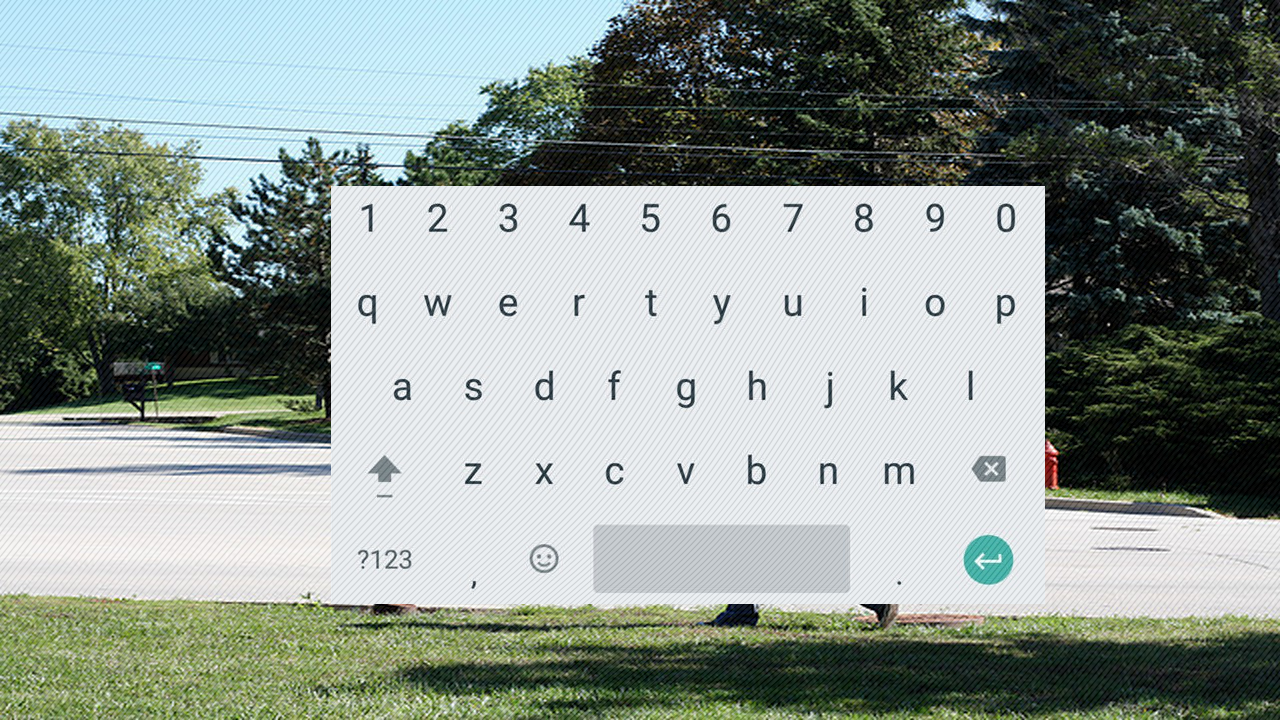
\includegraphics[width=7cm]{img/dataset/keyboard-bg-coco.png} }}
    \qquad
    \subfloat[\centering Average border color as a background]{{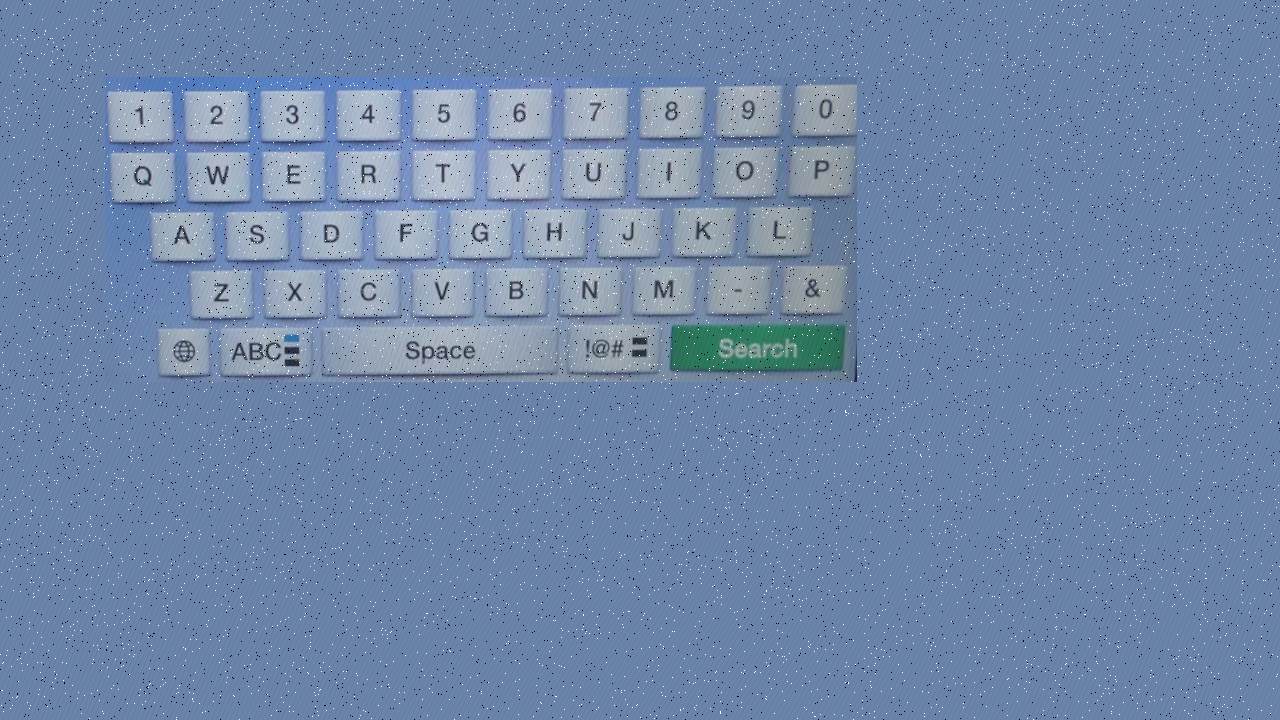
\includegraphics[width=7cm]{img/dataset/keyboard-bg-border.png} }}
    \vspace{-4pt}
    \caption{Comparison of~a COCO image (a) and keyboard border color (b) as~a background shows how the keyboard in~a scene clearly stands out.}
    \label{keyboard-bg-comparison}
\end{figure}

A keyboard is placed on~a background completely randomly. The only constraint is that it cannot overflow. Conditionally, the keyboard can get resized or made transparent and to~the whole image light conditions can be changed or noise added. Moreover, a random moiré effect is always computed as~the images under detection will be screenshots from~a camera. Section~\ref{dataset-keyboards-augmentation} referes about~these modifications in more detail. The whole process summarizes algorithm~\ref{keyboard-generation-algorithm}.

\begin{algorithm}
    \begin{algorithmic}[1]
    \STATE $keyboard\gets get\_keyboard()$
    \IF{$random() \leq 0.25$}
        \STATE $keyboard\gets resize(keyboard, random(0.5, 2))$
    \ENDIF
    \IF{$random() \leq 1/3$}
        \STATE $keyboard\gets make\_transparent(keyboard, random(0.5, 1))$
    \ENDIF
    \STATE $bg\gets get\_background()$
    \STATE $img\gets put\_keyboard\_on\_bg(keyboard, bg)$
    \IF{$random() \leq 0.5$}
        \STATE $img\gets change\_brightness(img)$
    \ENDIF
    \IF{$random() \leq 0.9$}
        \STATE $img\gets add\_random\_noise(img)$
    \ENDIF
    \STATE $img\gets add\_moire(img)$
    \end{algorithmic}
    \caption{Pseudocode for generation of single image for keyboards dataset}
    \label{keyboard-generation-algorithm}
\end{algorithm}

\subsection{Data augmentation}
\label{dataset-keyboards-augmentation}
Owing to~the office or lab conditions in~which AIVA operates, no natural elements like rain need to~be taken into~consideration. Moreover, thanks to~the camera calibration system, other modifications such as rotation or perspective can be omitted. In~the end, only various light conditions, noise and different moiré effects are the real problems. Apart from these, keyboard size and transparency with respect to~the background are also subjected to~the data augmentation process.

If we follow the algorithm~\ref{keyboard-generation-algorithm}, firstly the keyboard is resized. This happens with a~25~\% probability. The image can be changed to~any size in~the range of~twice as small to~twice as~big as~the original. However, boundaries are in~place, so that it cannot overflow the background. Next in~line is the transparency which is applied with probability~\(1/3\) and it is quite simple as the only thing necessary is adding the alpha channel. The alpha is chosen randomly from~interval \(\langle0.5, 1\rangle\). Both of~these modifications are applied directly on~the keyboard region itself, whereas the following augmentation methods concern the whole image.

To~simulate different light conditions, brightness change is applied to~every other image. For~that, gamma correction is used. Firstly, \(\gamma\) is picked from interval \(\langle0.5, 1.5\rangle\) where \(\gamma < 1\) makes the image darker and \(\gamma > 1\) makes it lighter. Secondly, \(\gamma\) is applied to~the image using equation~\ref{equation-gamma}. Image must be normalized from~\(\langle0, 255\rangle\) to~\(\langle0, 1\rangle\) for~the gamma application and than converted back. Figure~\ref{dataset-keyboards-augmentation-gamma} shows the difference between the dark, normal and light images.

\begin{equation}
  \label{equation-gamma}
  Output = \left(\frac{Img}{255}\right)^\frac{1}{\gamma} * 255
\end{equation}

\begin{figure}[tbh]
    \centering
    \subfloat[\centering \(\gamma\) = 0.5]{{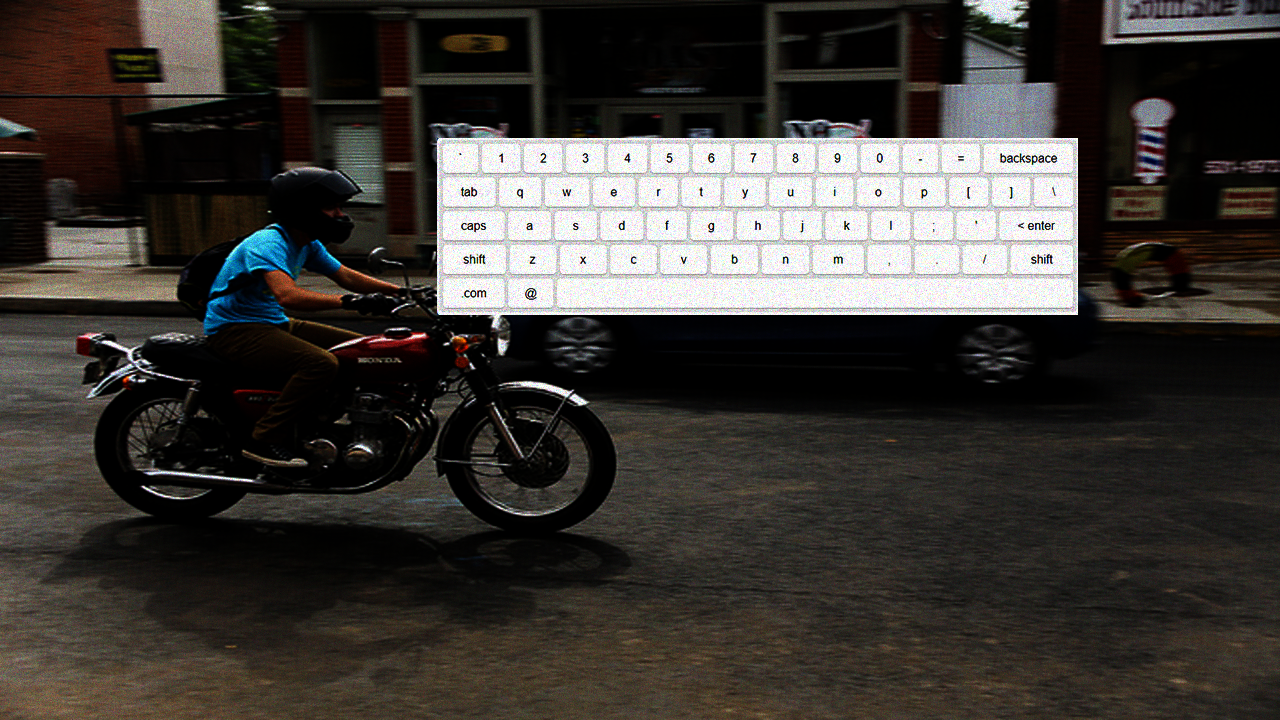
\includegraphics[width=4.95cm]{img/dataset/gamma-dark.png} }}
    \qquad \hspace{-2.34em}
    \subfloat[\centering \(\gamma\) = 1]{{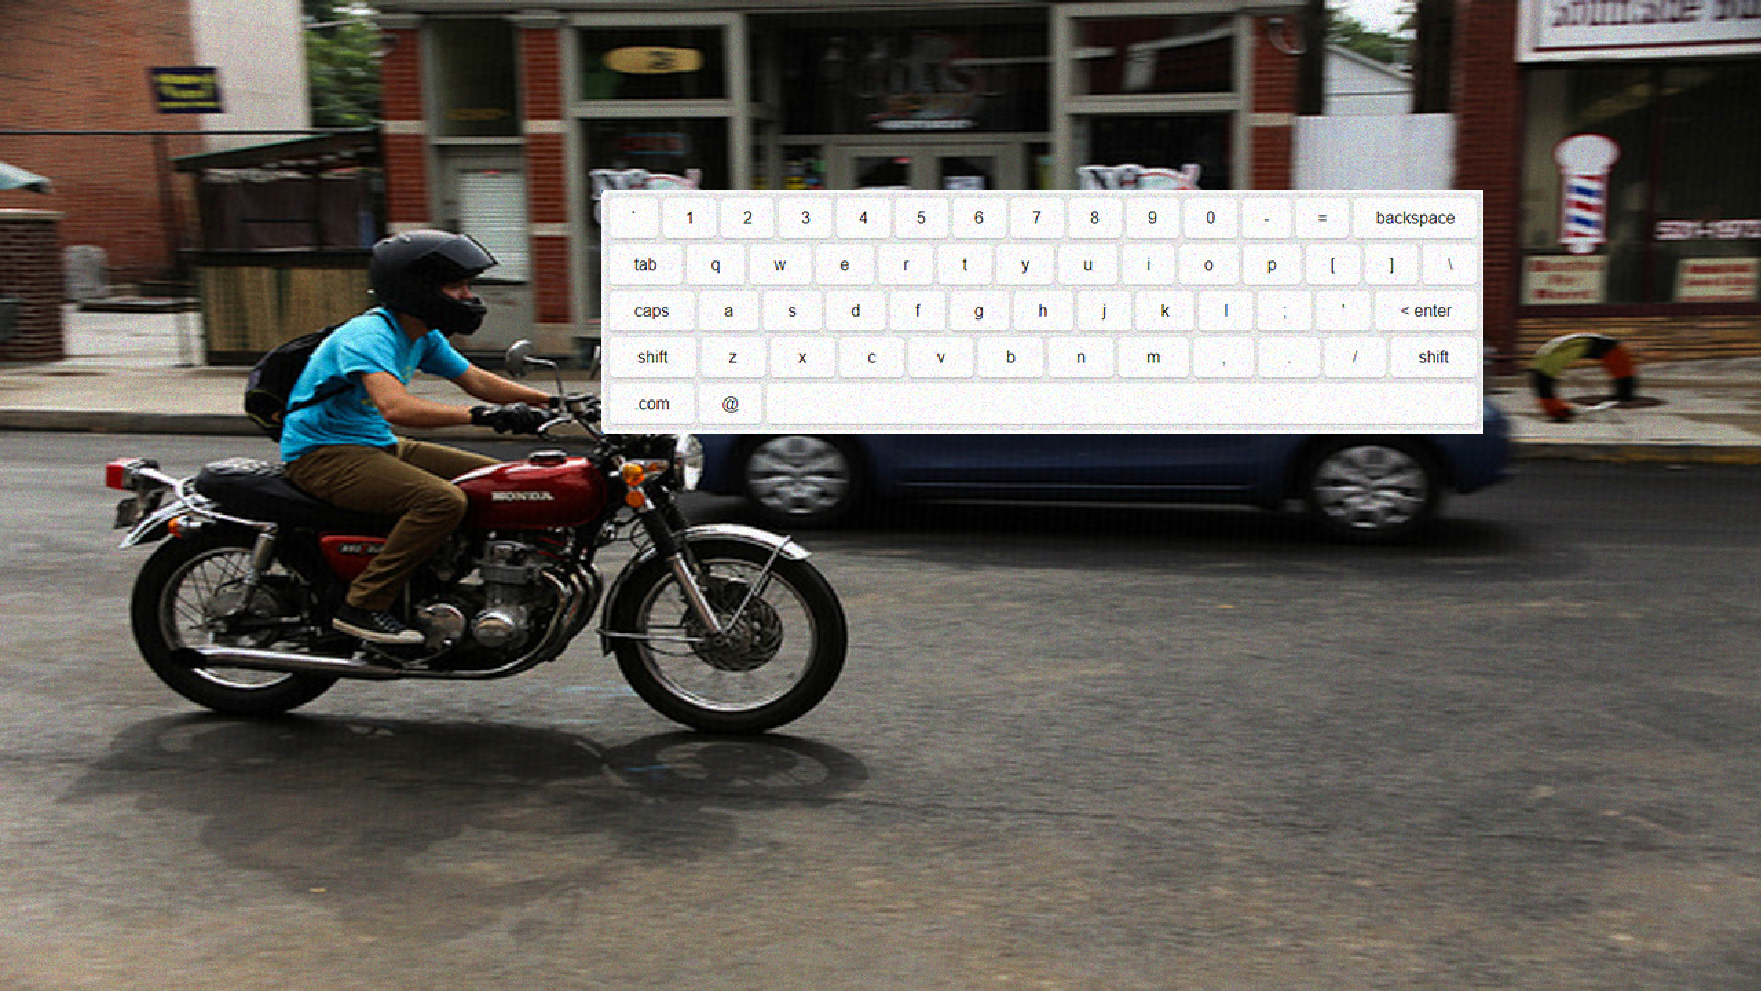
\includegraphics[width=4.95cm]{img/dataset/gamma-normal.pdf} }}
    \qquad \hspace{-2.34em}
    \subfloat[\centering \(\gamma\) = 1.5]{{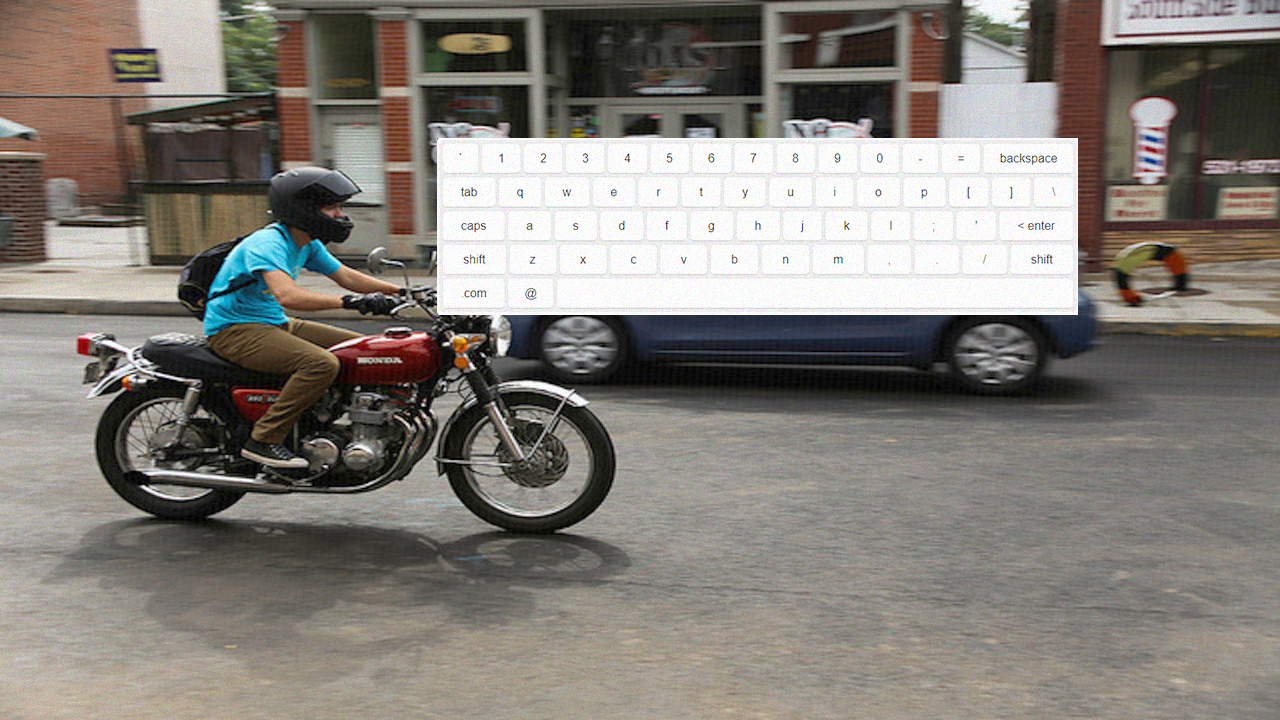
\includegraphics[width=4.95cm]{img/dataset/gamma-light.png} }}
    \caption{Comparison of~dark~(a), original~(b) and light~(c) versions of~an image. The resulting image of~the brightness change application can be anywhere in~between these values. Note that even brighter images would be viable for~most images, however, for~some, it could be too much, so these margins were selected for~both generalization and equal dark/light distribution.}
    \label{dataset-keyboards-augmentation-gamma}
\end{figure}

The next augmentation technique is noise addition. As~noise in an image is quite common, it is generated in~90~\% of them. Four types of~noise with~the same probability of occurrence were used. The first one is Gaussian noise. The Gaussian parameters are set to~\(\mu = 0\) and \(\sigma \in \langle0.5, 10\rangle\)~\ref{equation-gaussian-noise}. The randomly generated noise is then added to~the image.

\begin{equation}
  \label{equation-gaussian-noise}
  Img = Img + N(0, \sigma^2) \hspace{0.5cm} \sigma \in \langle0.5, 10\rangle
\end{equation}

The next one is Poisson noise. This noise makes the image very bright though, so the noise values are randomly divided by~a number from~\{2, 3, 4, 5, 6\} to~reduce its effect~\ref{equation-poisson-noise}.

\begin{equation}
  \label{equation-poisson-noise}
  Img = Img + \frac{Pois(Img)}{r} \hspace{0.5cm} r \in \{2, 3, 4, 5, 6\}
\end{equation}

Another noise is salt and pepper. It iterates through every pixel in~the image and with~a certain probability it sets a pixel to~white or black~\ref{equation-sp-noise}. This probability is again randomly chosen from~interval \(\langle0.005, 0.01\rangle\).

\begin{equation}
  \label{equation-sp-noise}
  Img[i] = \begin{dcases}
 0 & \text{if}\hspace{6pt}r < P
 \\
 255 & \text{if}\hspace{6pt}r > 1 - P
 \\
 Img[i] & \text{else}
 \end{dcases}
 \hspace{0.5cm} r \in \langle0.5, 10\rangle, P \in \langle0.005, 0.01\rangle
\end{equation}

The last one is speckle noise. To~generate such noise, the image is multiplied by~a random map from~the standard normal distribution and optionally can be multiplied by~a variance. The variance is again randomly chosen from~interval \(\langle0.05, 0.4\rangle\) and it controls the noise intensity. In~the end, it is added to~the original image~\ref{equation-speckle-noise}. A~comparison of~these~4~noises is shown in~figure~\ref{dataset-keyboards-augmentation-noise}. 

\begin{equation}
  \label{equation-speckle-noise}
  Img = Img + Img * N(0, 1) * var \hspace{0.5cm} var \in \langle0.05, 0.4\rangle\
\end{equation}

\begin{figure}[tbh]
    \centering
    \subfloat[\centering Gaussian noise]{{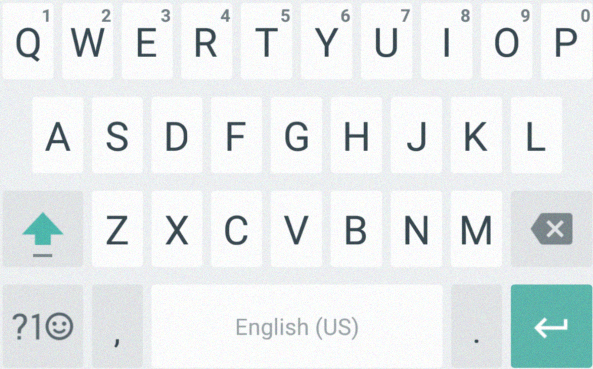
\includegraphics[width=7cm]{img/dataset/noise-gauss.png} }}
    \subfloat[\centering Poisson noise]{{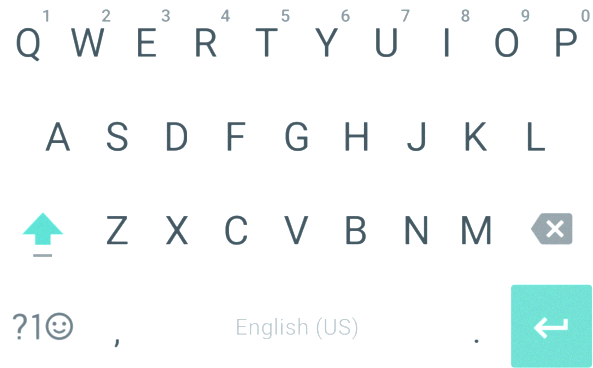
\includegraphics[width=7cm]{img/dataset/noise-poisson.png} }}
    \quad
    \subfloat[\centering Salt and pepper noise]{{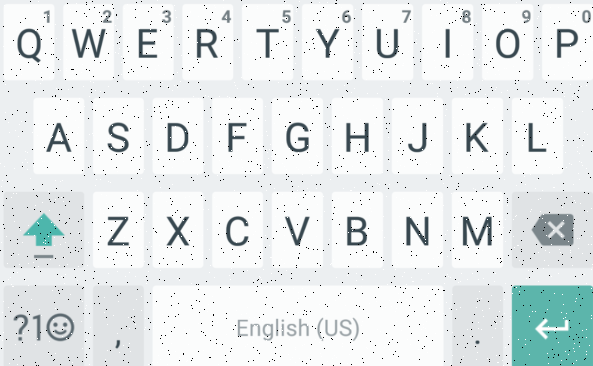
\includegraphics[width=7cm]{img/dataset/noise-sp.png} }}
    \subfloat[\centering Speckle noise]{{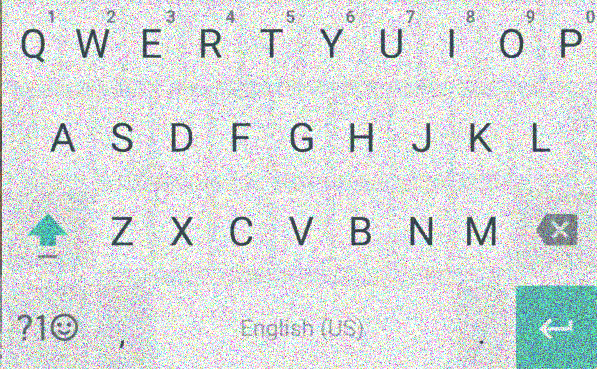
\includegraphics[width=7cm]{img/dataset/noise-speckle.png} }}
    \caption{Comparison of~Gaussian (a), Poisson (b), S\&P (c) and speckle (d) noises}.
    \label{dataset-keyboards-augmentation-noise}
\end{figure}

The final data augmentation method is moiré effect generation. This is particularly \hbox{important} as~the image subjected to~the object detection is usually a target device screen taken by~a camera which tends to~exhibit moiré pattern behaviour. To~create a moiré effect in~an image, python \texttt{latticegen} library~\cite{latticegen} and especially method \texttt{anylattice\_gen(r\_k, theta, order, symmetry)} was used. It is capable of~creating parameterized moiré lattices. To~set the lattice scale (how big or seemingly zoomed the lattice is) there is \texttt{r\_k} \hbox{parameter} which I select randomly from interval \(\langle0.01, 0.25\rangle\). Parameter \texttt{theta} stands~for~\hbox{lattice} \hbox{rotation} and it can be anything between~0 and~90~degree angle. The \texttt{order} parameter is for~simplicity described as \say{The higher the order, the more well-resolved the atoms are as~single spots}~\cite{latticegen} which can be seen in~figure~\ref{latticegen-order}. One of~the first~3 orders is randomly chosen for~the generation.

\begin{figure}[hbt]
    \centering
    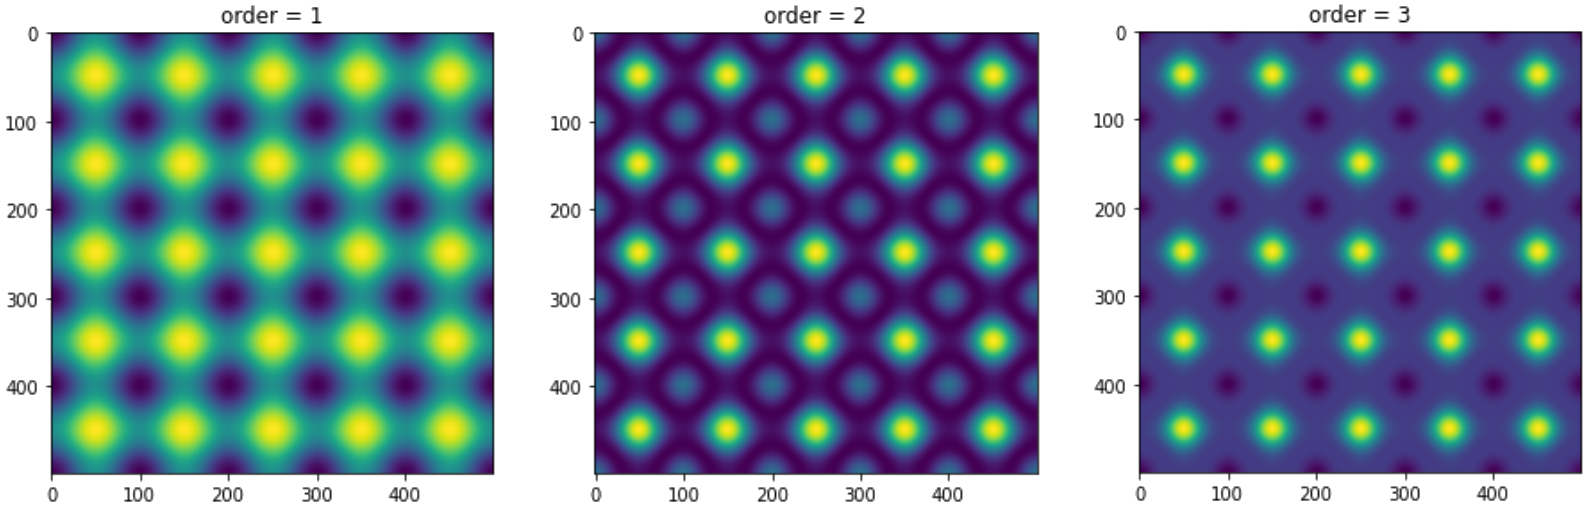
\includegraphics[width=0.98\textwidth]{img/dataset/latticegen-order.png}
    \caption{Different latticegen orders (adapted from~\cite{latticegen})}
    \label{latticegen-order}
\end{figure}

The last parameter \texttt{symmetry} controls the shape of~the spots. The most common moiré effect on~screens seems to~be lines which correspond to~symmetry value~1. For~that reason, the value~1 is chosen in~50~\% of~cases. The rest is equally distributed to~values \{2, 3, 4, 5\}. Different symmetries depicts figure~\ref{latticegen-symmetry}.

\begin{figure}[hbt]
    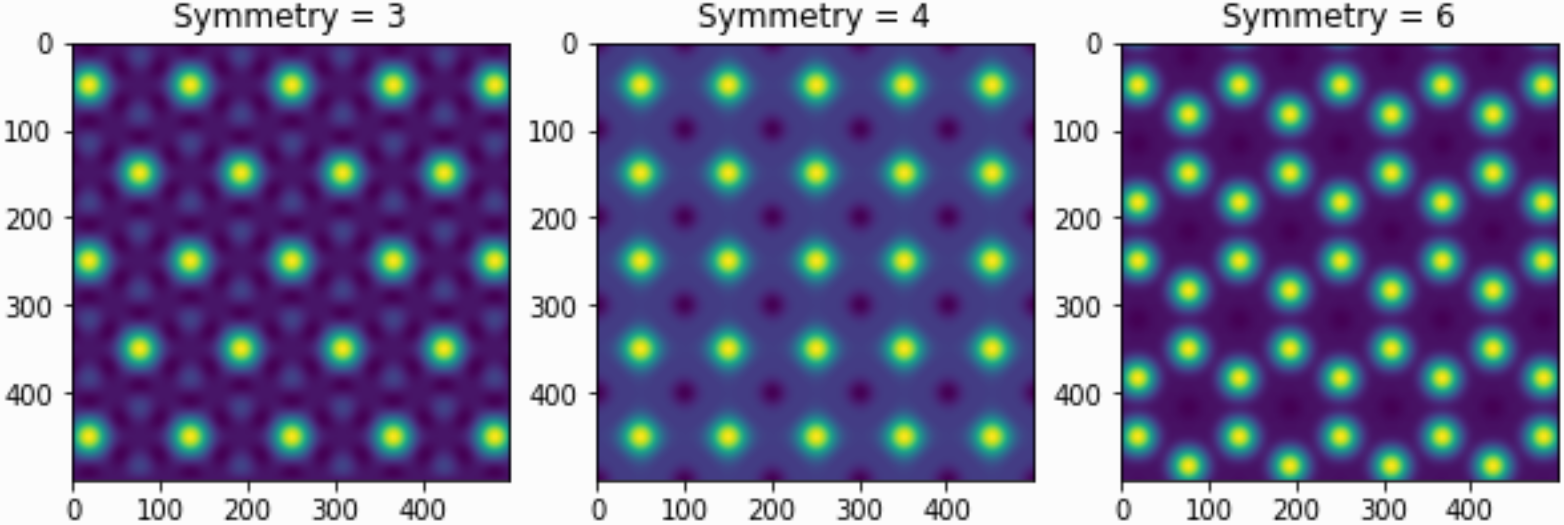
\includegraphics[width=1\textwidth]{img/dataset/latticegen-symmetry.png}
    \caption{Different latticegen symmetries (taken from~\cite{latticegen})}
    \label{latticegen-symmetry}
\end{figure}

So that the lattice is not always regular, a shift taken from the library is applied. For~the shift, no further randomization is done as~it behaves differently on~various lattice designs. To~deform the regularity even more, several lattices can be combined together. In~the end, either a single lattice or a combination of~2 lattices is used with equal probability.

\section{Characters}
\label{dataset-characters}
In~many ways, the generation of~characters dataset is the same as~the one for~the keyboards. Some characters are selected, put on~a background and then noise and moiré effect are added. Noise is created similarly as~to the keyboard images. The only difference is that additional gaussian noise is added with 50~\% probability. Concerning the moiré effect, the lattice is always of the first order and the symmetry is always~1 (lines) as~the special patterns empirically did not influence the image much. Gamma correction is omitted because the characters dataset is in~grayscale, so the brightness naturally differs simply by~choosing different gray colors. There are several reasons for~grayscale images. The most important one is that the keyboards are very contrastive. By converting to~grayscale, the characters will always be light on~a dark background or vice versa no matter the original color design. Another reason is that processing a grayscale image is easier than a colored one. In~addition, to~simulate bad-quality images, every third image is blurred by~scaling down (randomly up to half) and up again. The algorithm~\ref{characters-generation-algorithm} demonstrates the process.

\begin{algorithm}
    \begin{algorithmic}[1]
    \STATE $char\gets select\_character()$
    \STATE $bg\gets generate\_background()$
    \STATE $img\gets put\_characters\_on\_bg(char, bg)$
    \IF{$random() \leq 0.5$}
        \STATE $img\gets add\_gaussian\_noise(img)$
    \ENDIF
    \IF{$random() \leq 0.95$}
        \STATE $img\gets add\_random\_noise(img)$
    \ENDIF
    \STATE $img\gets add\_moire(img)$
    \IF{$random() \leq 1/3$}
        \STATE $img\gets blur(img)$
    \ENDIF
    \end{algorithmic}
    \caption{Pseudocode for generation of single image for characters dataset}
    \label{characters-generation-algorithm}
\end{algorithm}

Having described the high level differences to~the keyboards dataset generation, the rest of~this section focuses on~the selection and placement of~the characters on~the background. The set of~characters consists of~alphanumeric ones (a-zA-Z0-9), special characters from the sequence .,:;'"?!@\#\$£€\%\^{ }\&()\{\}[]<>/\textbackslash\_+-*÷= and icons for~backspace, shift, enter, space and tab. These are repeatedly iterated during the dataset generation. For~further reference, an iteration's current character is considered to~be the \say{main character}. The background on~which the characters are placed is created as~follows. The resolution is set to 640x640 for several reasons. A keyboard usually takes around~\(1/2\) of~the screen's height so the target resolution~1920x1020 is covered. Moreover, object detectors take square images and the current state-of-the art YOLOv7 uses 640x640. Furthermore, the objective is to find characters of different but bounded sizes, so the background resolution does not play a significant role anyway. As~for~the background color, it is usually light or dark. The background color probability is shifted towards such pixel intensities on~the gray scale according to~the formula~\ref{equation-bg-grayscale}.

\begin{equation}
  \label{equation-bg-grayscale}
  bg\_color = \begin{dcases}
 randInt(0, t) & \text{if}\hspace{6pt}r \leq \frac{1}{3}
 \\
 randInt(255 - t, 255) & \text{if}\hspace{6pt}r \in (\frac{1}{3}, \frac{2}{3}\rangle
 \\
 randInt(0, 255) & \text{else}
 \end{dcases}
 \hspace{0.5cm} r \in \langle0, 1\rangle, t = 64
\end{equation}

A convenient threshold \(t\) for~the light/dark boundaries appeared to~be value~64. The formula~\ref{equation-bg-grayscale} basically says that with~a~\(1/3\) chance the background color will be dark, with~another~\(1/3\) chance that light or else it will be completely random.

The placement of~characters on~a background is a bit more complicated. The main character is rendered several times on the background and other random characters with~it. Different position, color and font, which includes font family, size, weight and style, are selected for~each character. To~solve the position selection, an attempt to~just randomly put characters on~the background and check for~intersections was made in~the beginning. However, the intersections occurred so often that too few characters could be safely rendered which left a lot of~free space. As~a consequence, a grid system was devised. The largest font size used is~64 which means that after dividing the resolution, from which a random padding is subtracted so that the characters are not directly on~a border, a~9x9 grid is created. In~order to render not only individual characters but words as~well, one or~two lines are randomly left out of~the grid for~word generations. This is because a detector might otherwise not learn to~recognize characters in~the proximity of~other characters. The generated words are either keyboard special words (space, shift, enter...), mode-changing sequences (abc, ?123, \#+=...) or completely random character sequences. Out of~the remaining (7|8)x9~=~63-72 grid cells, a quarter to~half is randomly taken by the main character and another quarter to~half by~other random characters. As~a result, there is no intersection and even the grid is not that apparent as~not all grid cells are utilised and different characters of~various fonts and sizes are rendered.

Concerning the color selection, the contrast between the characters and keyboard/key background is usually very high, often even black on~white and vice versa. Thus, a pixel intensity threshold for~the difference between the background and a character color can be set. The formula~\ref{equation-font-color} demonstrates the calculation of~available colors to~be randomly chosen from, where \(I_{bg}\) is the intensity of~the background pixels and \(t\) stands for~the threshold. In~75~\% of~cases, the threshold value is~92 due to~the high contrasts and~24 otherwise so~that even unusual low contrastive keyboards can be learned. The visual difference between the threshold pixel intensities with respect to~different backgrounds provides figure~\ref{font-color-selection}.

\begin{equation}
  \label{equation-font-color}
  available\_colors = \langle0, 255\rangle \setminus \langle I_{bg} - t, I_{bg} + t\rangle \hspace{0.5cm} t \in \{24, 92\}
\end{equation}

\begin{figure}[tbh]
    \centering
    \subfloat[\centering I(24) on I(0)]{{
\includegraphics[width=3.5cm]{img/dataset/font-color-dark-light-24.png} }}
    \subfloat[\centering I(92) on I(0)]{{
\includegraphics[width=3.5cm]{img/dataset/font-color-dark-light-92.png} }}
    \subfloat[\centering I(255-24) on I(255)]{{
\includegraphics[width=3.5cm]{img/dataset/font-color-light-dark-24.png} }}
    \subfloat[\centering I(255-92) on I(255)]{{
\includegraphics[width=3.5cm]{img/dataset/font-color-light-dark-92.png} }}
    \\[-6pt]
    \subfloat[\centering I(128-24) on I(128)]{{
\includegraphics[width=3.5cm]{img/dataset/font-color-middle-dark-24.png} }}
    \subfloat[\centering I(128-92) on I(128)]{{
\includegraphics[width=3.5cm]{img/dataset/font-color-middle-dark-92.png} }}
    \subfloat[\centering I(128+24) on I(128)]{{
\includegraphics[width=3.5cm]{img/dataset/font-color-middle-light-24.png} }}
    \subfloat[\centering I(128+92) on I(128)]{{
\includegraphics[width=3.5cm]{img/dataset/font-color-middle-light-92.png} }}
    \caption{The first row shows~24 and~92 pixel intensity I(x) differences on~a black/white background. The second row depicts the same for~a middle gray background bidirectionally.}
    \label{font-color-selection}
\end{figure}

With~regards to~the font selection, 46~different font families such as~Calibri, Arial, Verdana etc. are used. For~most of~them, bold and italic versions are available. As~italic characters are quite uncommon on~keyboards, the normal to~italic ratio is~95:5. On~the other hand, bold characters are seen more often, so a bold font is used in~40~\% of~cases instead~of the regular one. Font size is selected from~interval \(\langle8, 64\rangle\) with~a~50~\% chance of~inclination towards the lower half.

As~there are several characters in~an image, the annotation file format needed to~be changed. Like in~the keyboards annotation, the dictionary key is a filename, however, the value is not a single bounding box for~a single keyboard in~an image, but another dictionary for~characters. In~the value dictionary, keys are individual characters and values are lists of~bounding boxes as~figure~\ref{characters-annotation-json} shows.

Totally, 40~000 character images are generated with train-validation-test ratio~70:20:10 and an example is shown in figure~\ref{dataset-characters-image}. In~the training set, there are 2~287~613 characters. As~there are~99 of~target classes, each one has on~average~23~107 representations. This is significantly more than my Amazon counterparts who manually annotated characters on~634~keyboards~\cite{amazon-paper}. As~they work with~68~characters and~26~(a-z~vs~A-Z) are usually mutually exclusive, there could be a maximum of~42~characters in~each image which results in 634x42=26~628 characters. If uniform distribution of~characters is presumed, it makes 26~628/68=391 samples for~each character. However, from~my findings lowercase characters are more usual in~internet keyboard images, so the uniform distribution is doubtful. The benefits of~my dataset are the following:

\begin{itemize}[topsep=0pt,itemsep=-1.5pt,partopsep=6pt]
    \item There is substantially more samples for~each character.
    \item Any character can be generated, not just what is found in~an internet image.
    \item Characters are generated uniformly, none has significantly more samples than others.
    \item There is no need for~manual annotation.
\end{itemize}

\vspace{-6pt}
\begin{figure}[!hbt]
    \centering
    \begin{boxedverbatim}
"27.png": {
    "A": [
        [463, 193, 491, 223],
        [95, 105, 126, 132],
        [3, 382, 36, 415],
        ...
    ],
    "n": [
        [463, 115, 510, 161],
        [279, 380, 310, 427]
    ],
    ...
},
"28.png": {
    ...
},
...
\end{boxedverbatim}
    \vspace{-6pt}
    \caption{Characters annotation file is a JSON dictionary with a filename as~a key and a dictionary of character~bounding boxes in~format [x1, y1, x2, y2] as~a value.}
    \label{characters-annotation-json}
\end{figure}

\vspace{-12pt}
\begin{figure}[!hbt]
    \centering
    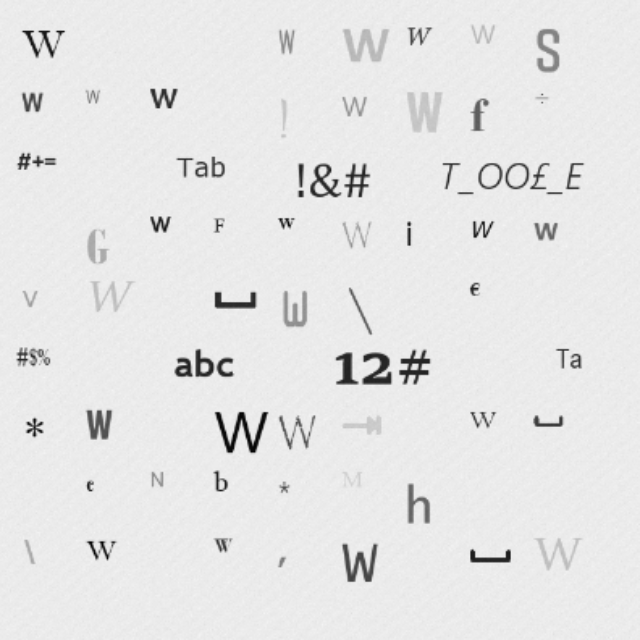
\includegraphics[width=0.66\textwidth]{img/dataset/characters-img-W.png}
    \vspace{-6pt}
    \caption{An image from characters dataset with W as~the main character}
    \label{dataset-characters-image}
\end{figure}

\section{Post-processing}
\label{dataset-postprocessing}

In~comparison with~the previous ones, the post-processing dataset serves only for~validation and is substantially smaller. There are~2~major issues which need to~be solved after the actual detection. The first one is that a lot~of times more than one character is written on~a key. On~a physical keyboard, the other character(s) is usually accessed by~switching keyboard language or by~pressing the shift key. On~digital keyboards, they mostly just foreshadow what special character is in~another keyboard mode. For~my problem, only the main keyboard character is relevant as~AIVA's robotic arm cannot press multiple buttons. Therefore, these other characters need to~be recognized and discarded based on~the keyboard layout. The second issue is that not all characters will necessarily be detected or recognized correctly e.g.~'o'~vs~'O'~vs~'0'. This needs to~be solved in~post-processing and a proper validation dataset must be provided for~such a task.

From~the collected keyboard regions,~120~which are appropriate to~test these issues are selected. These are further split 50:50 into~2~groups. The first group is called \emph{layout} and it validates the correct detection of~characters on~different keyboard layouts, including the omission of~unwanted characters. The second one is named \emph{missing\_chars} where not only single characters but also sequences of~characters are removed to~test if they can be automatically computed. Moreover, even characters in keywords (e.g.~\emph{space}) are left out~to~test partial recognition of~keywords for~special keys.

  \chapter{Keyboard and keys detection design and implementation}
\label{design-and-implementation}

Among the thesis requirements is not only the keys detection to~allow automated typing but also individual keyboard detection so~that a decision if an AIVA unit sees a keyboard screen can be made. For~that reason, a similar approach to~the one described in~the Amazon paper~\cite{amazon-paper} is appropriate. In~this chapter, a three-phase strategy for~automated keyboard typing using current SOTA methods is proposed. Firstly, a keyboard region is detected using the latest YOLO version as~described in~section~\ref{design-keyboard}. Making it a separate subtask, said requirement for~keyboard screen recognition is satisfied. Secondly, keys are detected in~the identified keyboard region which simplifies the recognition in~comparison to~finding the keys in~the whole image. This process presented in sections~\ref{design-keys} and~\ref{design-keys-postprocessing} covers the second and third phases, character detection and post-processing corrections respectively. The whole recognition is reviewed and demonstrated in~the last section~\ref{design-final-detection-process}. Unfortunately, this design cannot be tested against the Amazon's solution as~neither the code nor~the dataset is to~the best of~my knowledge available. This fact makes this work even more contributive, as~no other seems to~currently exist on~the topic.

\section{Keyboard detection}
\label{design-keyboard}
This task can be seen as~a standard object detection with~just a single class to~recognize, a~keyboard. The Amazon researchers used SSD300 neural network with~great results. Since then, a newer, faster and more accurate architecture has been devised which is YOLOv7. While YOLOv7 was briefly introduced in~section~\ref{algorithms-nn-yolo}, as~a selected model architecture, the following section~\ref{design-keyboard-neural-network} describes it in~more depth. Section~\ref{design-keyboard-implementation} demonstrates, how the model was trained and how it can be used.

\subsection{Neural network design for keyboard detection}
\label{design-keyboard-neural-network}
The YOLOv7 paper clearly states that it derives from~the state-of-the-art (SOTA) \hbox{methods} and aims to~improve loss function, label assignment and training~\cite{yolov7}. Hence, the focus is directed on~the incremental changes as~the base architecture of~SOTA YOLO at~the time from~figure~\ref{design-yolo-architecture} is already described in~section~\ref{algorithms-nn-yolo}. YOLOv7 introduces~4~\hbox{major} changes, two architectural (E-ELAN, Model scaling for concatenation-based \hbox{models}) and two trainable bag-of-freebies (Planned re-parameterized convolution, Coarse for~\hbox{auxiliary} and fine for~lead loss).

\begin{figure}[hbt]
    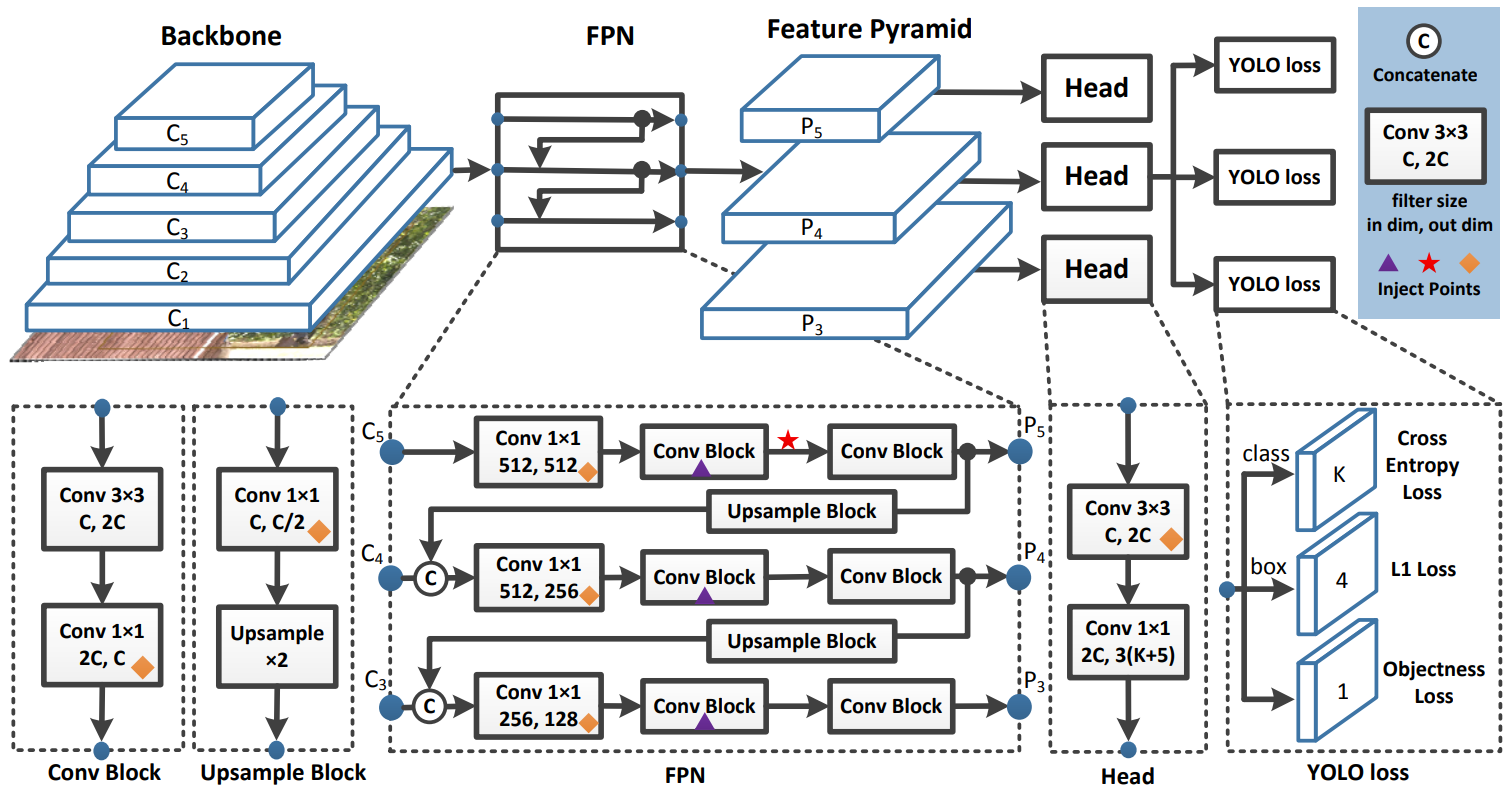
\includegraphics[width=1\textwidth]{img/design/yolov7-architecture.png}
    \caption{General YOLO architecture from~which YOLOv7 derives (taken from~\cite{pp-yolo}).}
    \label{design-yolo-architecture}
\end{figure}

\subsubsection{E-ELAN (Extended efficient layer aggregation network)}
The backbone consists of~E-ELAN computational blocks which depicts figure~\ref{design-yolo-eelan}. These blocks can be stacked and the depth of~the backbone can vary. There were implemented several models (YOLOv7-[X|W6|E6|D6|E6E]) of~different depths which are more accurate but slower respectively~\cite{yolov7}. The blocks are improvements of~ELAN blocks about which not much is known as the paper is not released yet at~the time of~writing of~this thesis. Nevertheless, they are supposed to~help control the longest shortest gradient path to~achieve more effective convergence~\cite{yolov7}. However, they have problems with~scaling and E-ELAN solves it using expand, shuffle and merge feature cardinality~\cite{yolov7}. For~the cardinality expansion, group convolution is used and for~more diverse learning, features of~different groups are shuffled and merged. Thus, more efficient learning is reached while only the inner block architecture is modified and not the outside so the gradient path is unchanged~\cite{yolov7}.

\vspace{-12pt}
\begin{figure}[!hbt]
    \centering
    \subfloat[\centering ELAN]{{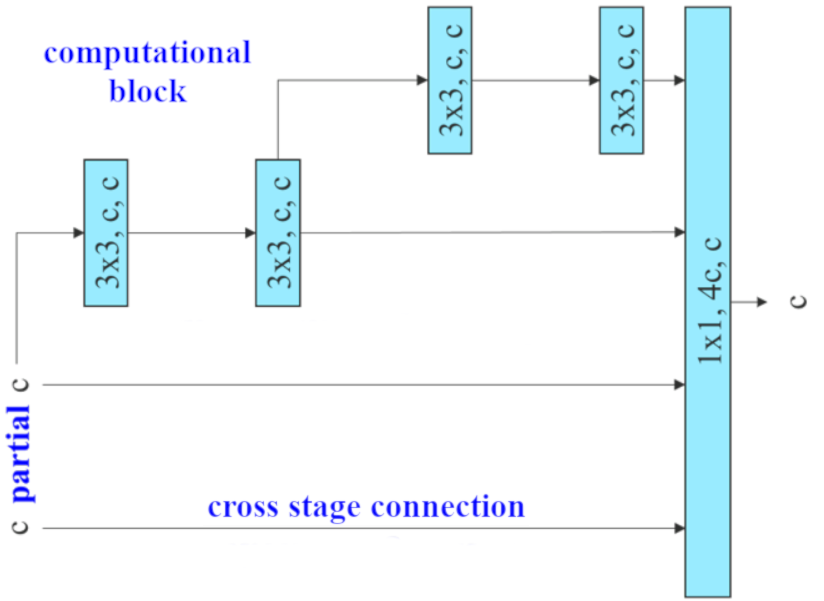
\includegraphics[width=7.45cm]{img/design/yolov7-elan.png} }}
    \subfloat[\centering E-ELAN]{{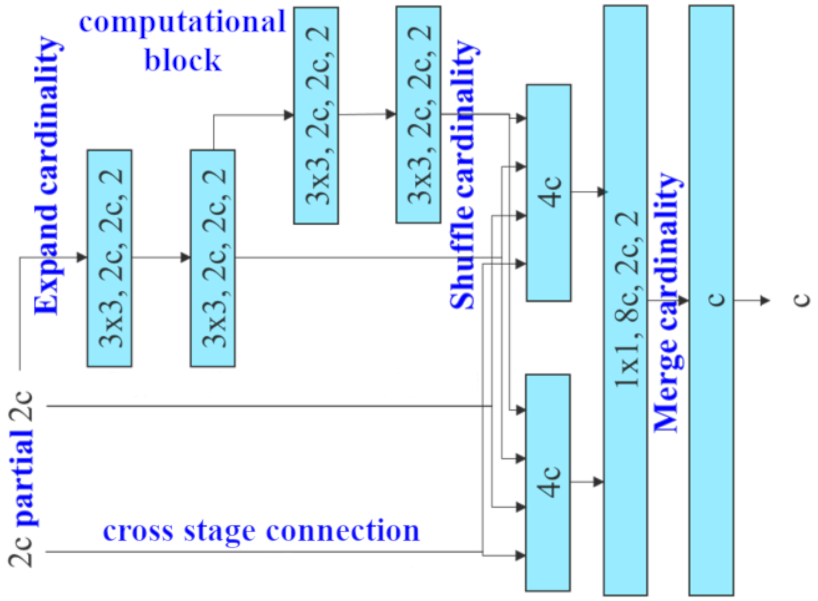
\includegraphics[width=7.45cm]{img/design/yolov7-e-elan.png} }}
    \vspace{-7pt}
    \caption{Difference between the ELAN block upon which YOLOv7 builds and Extended ELAN with~expand, shuffle and merge cardinality blocks (adapted from~\cite{yolov7}).}
    \label{design-yolo-eelan}
\end{figure}

\subsubsection{Model scaling for~concatenation-based models}
When a concatenation-based model is scaled by depth, the output width increases as (a) and (b) in~figure~\ref{design-yolo-scaling} demonstrate. Such changes usually affect the structure of~a model. To~maintain the initial properties of~the original design, a novel scaling method as (c) in figure~\ref{design-yolo-scaling} is~proposed which scales depth and width together~\cite{yolov7}.

\begin{figure}[hbt]
    \centering
    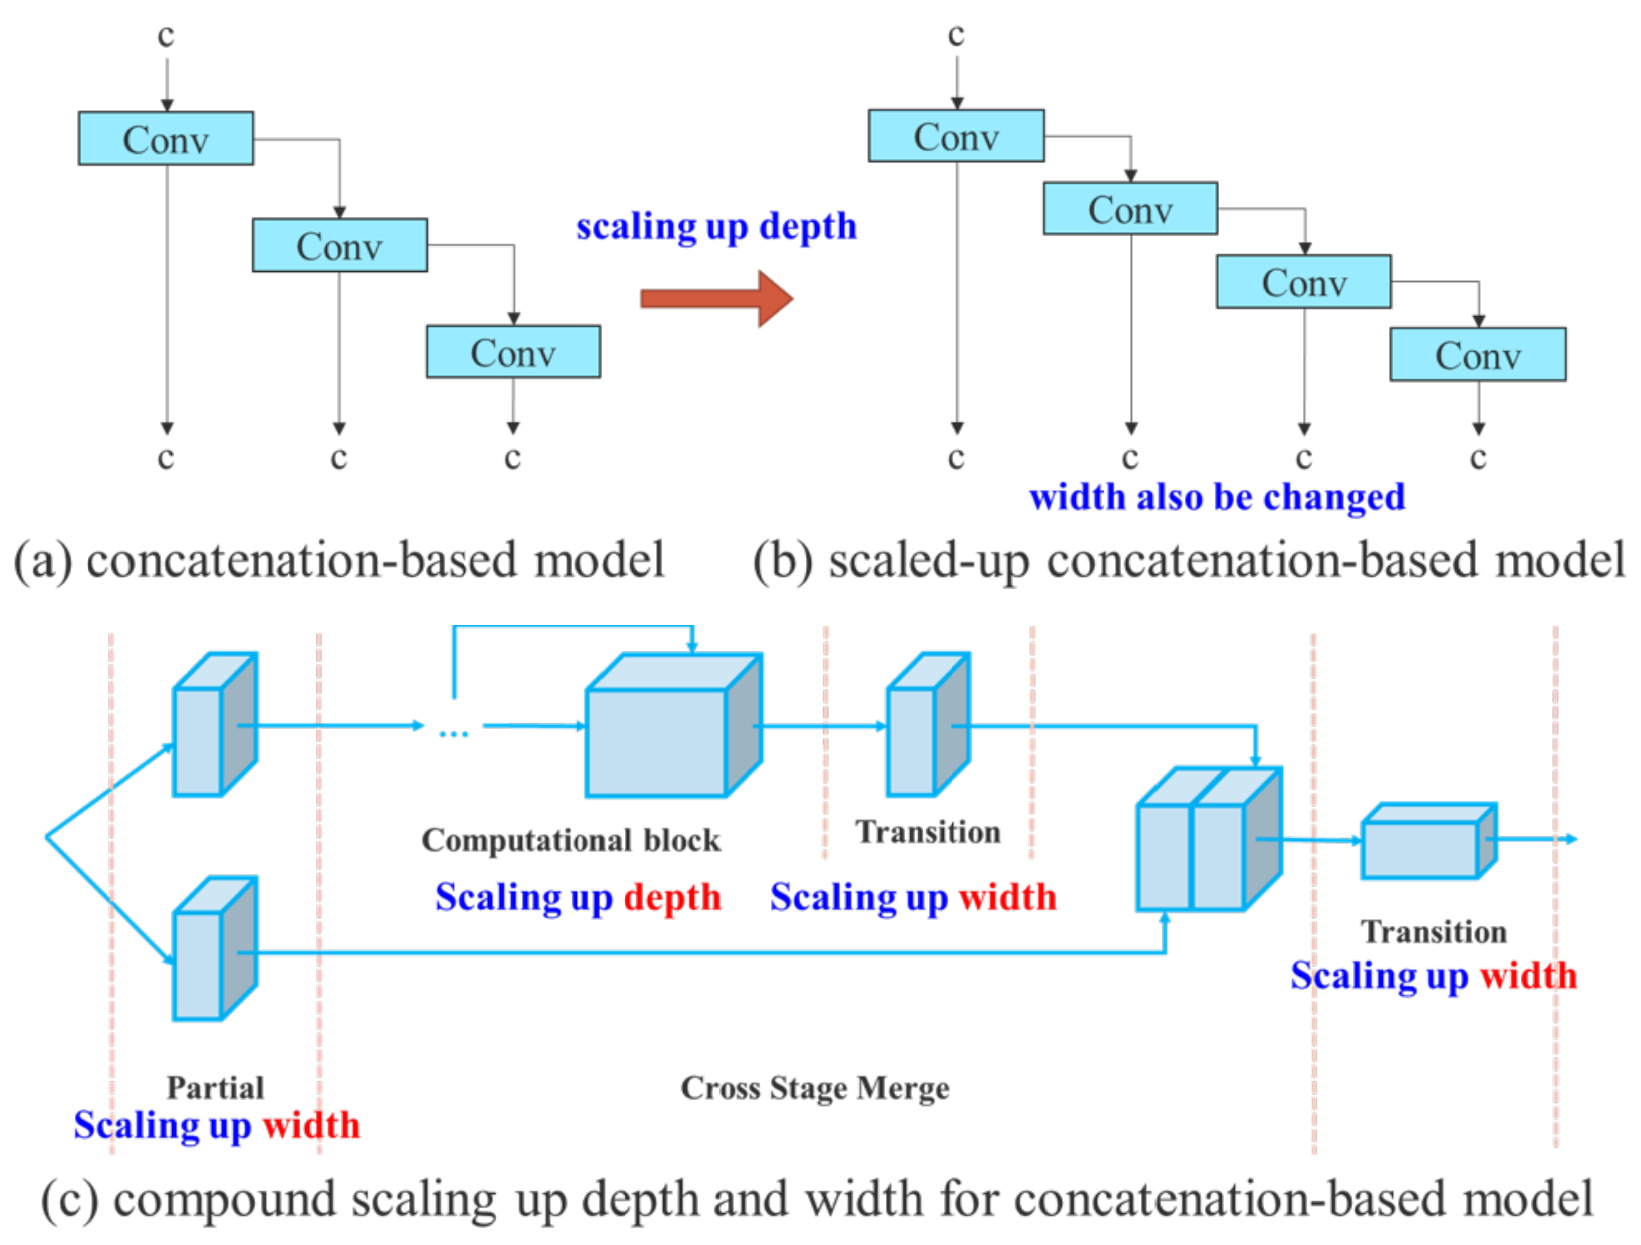
\includegraphics[width=0.9\textwidth]{img/design/yolov7-scaling.png}
    \caption{Depth scaling is required only inside of~a computational block and then the transition layer width is scaled according to~the output channel change~\cite{yolov7} (adapted from~\cite{yolov7}).}
    \label{design-yolo-scaling}
\end{figure}

\subsubsection{Planned re-parameterized convolution}
The purpose of~model re-parameterization is to~merge several computational modules \hbox{during} the inference stage by~averaging weights to~get a more robust module~\cite{yolov7}.
The previous YOLO version used heavily RepConv~\cite{rep-conv} which is a novel highly accurate classification architecture. RepConv combines 3x3 and 1x1 convolutions with~identity connection in~a single convolutional layer~\cite{yolov7}. However, the authors of~YOLOv7 discovered that in~combination with~other architectures such as~ResNet or DenseNet the accuracy is reduced~\cite{yolov7}. They further analyzed re-parameterized convolutions using gradient flow propagation paths in~order to~find out how they should be combined with~different networks. They discovered that RepConv doesn't perform well in~layers with~residual or concatenation connections. Figure~\ref{design-yolo-reparameterization} shows combinations which do or do not work. Hence, they proposed RepConvN (RepConv without the identity) to~be used instead in~such scenarios.

\vspace{-2pt}
\begin{figure}[!hbt]
    \centering
    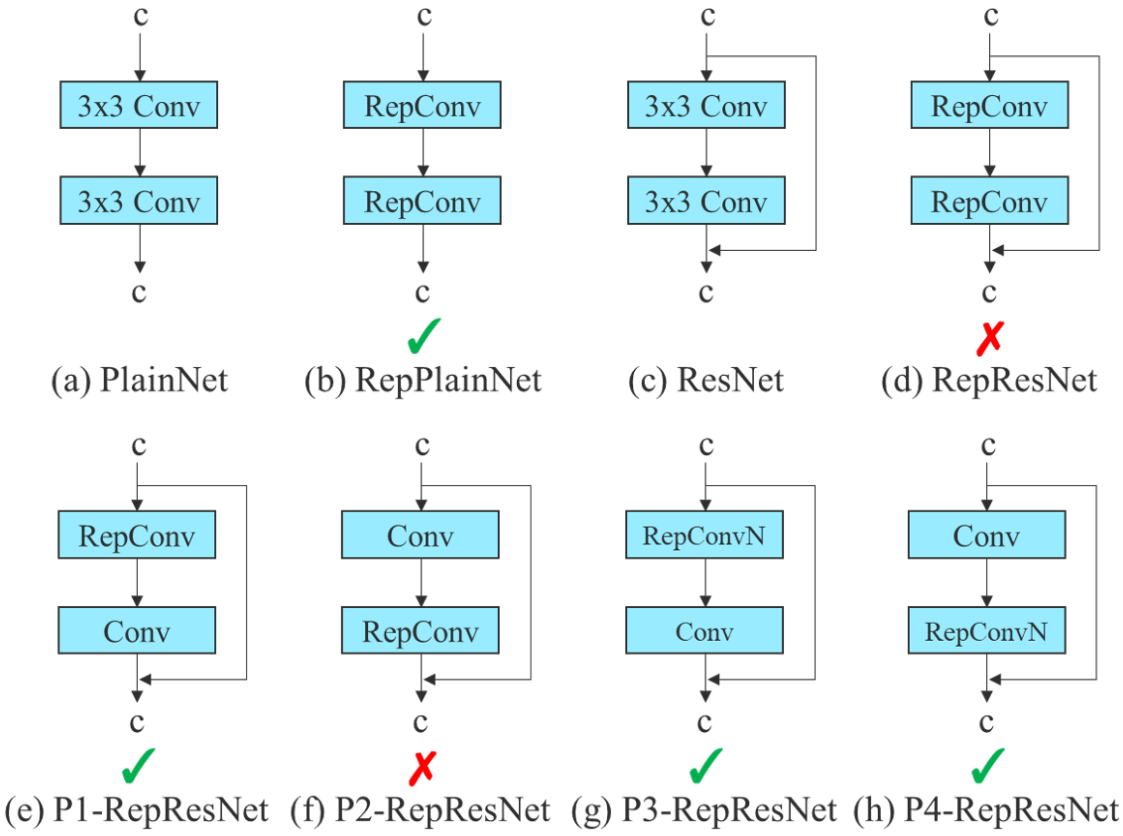
\includegraphics[width=0.7\textwidth]{img/design/yolov7-reparameterization.png}
    \caption{Architectures (not) working with~identity connections (taken from~\cite{yolov7}).}
    \label{design-yolo-reparameterization}
\end{figure}

\subsubsection{Coarse for~auxiliary and fine for~lead loss}
YOLOv7 introduces deep supervision~\cite{deep-supervision} to~the YOLO architecture. Figure~\ref{design-yolo-heads}~(a) depicts how auxiliary heads are added to~the model. In~general, the lead heads
are still responsible for~the final prediction, the auxiliary heads just help with~the training. While figure~\ref{design-yolo-heads}~(b) shows the popular approach at~the time that both heads make their own prediction, the proposed method in~YOLOv7 is to~guide both heads by~lead head prediction using (c) and (d) assigners~\cite{yolov7}. The paper describes them followingly. Lead guided assigner takes ground truth and lead head predictions and generates soft labels which are used as~targets for~both lead and auxiliary heads during the training. This way, the shallower auxiliary head can learn the predictions from~a more accurate lead head and the lead head can in~turn focus on~not yet learnt information. Coarse-to-fine lead head guided assigner also uses lead head predictions but creates~2~sets of~labels. Fine labels are the same as~soft labels in~the previous assigner. Coarse labels are generated with~lesser constraints for~positive sample assignment as~auxiliary heads have weaker learning capabilities and this can help to~avoid information loss.

\begin{figure}[hbt]
    \centering
    \subfloat[\centering Model with auxiliary heads]{{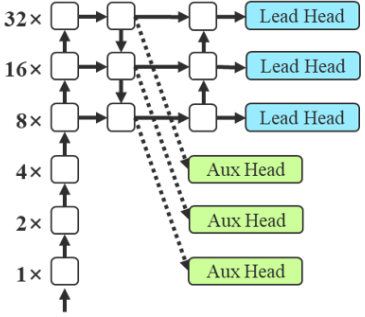
\includegraphics[width=6cm]{img/design/yolov7-heads-auxiliary-heads.png} }}
    \subfloat[\centering Independent assigner]{{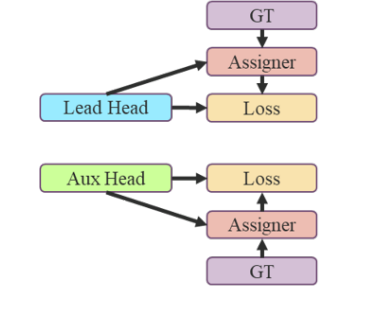
\includegraphics[width=6cm]{img/design/yolov7-heads-indipendent-assigner.png} }}
    \\
    \subfloat[\centering Lead guided assigner]{{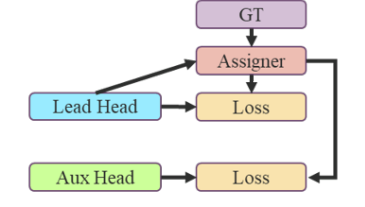
\includegraphics[width=6cm]{img/design/yolov7-heads-guided-assigner.png} }}
    \subfloat[\centering Coarse-to-fine lead guided assigner]{{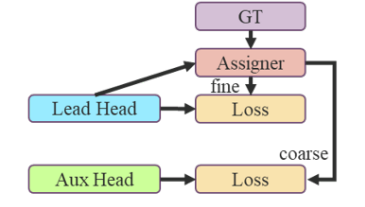
\includegraphics[width=6cm]{img/design/yolov7-heads-coarse-to-fine.png} }}
    
    \caption{Deep supervision adds auxiliary heads to~the middle of~a model (a). Label assigners are usually independent for~both lead and auxiliary heads (b), but YOLOv7 introduces assigners for~both heads (c, d)~\cite{yolov7} (adapted from~\cite{yolov7}).}
    \label{design-yolo-heads}
\end{figure}

\subsection{Training and usage of the detector}
\label{design-keyboard-implementation}
The YOLOv7 paper implementation is available on~GitHub\footnote[1]{\url{https://github.com/WongKinYiu/yolov7}} and is written using \hbox{PyTorch}. Hence the implementation of~the whole thesis is in~Python as well. The usage of~YOLOv7 is very straightforward and is shown by~algorithm~\ref{yolov7-code}. Firstly, one must install Python requirements (dependent libraries) either globally or in~a virtual environment, which is recommended. Secondly, a training run can optionally be initialized in the Weights \& Biases platform which the YOLOv7 project uses for logging and metrics collection. In~the code~\ref{yolov7-code}, this is done from Python while the other commands are for the command line, which is legit if using a Jupyter notebook for instance. Lastly, training itself can start.

\begin{algorithm}[!hbt]
    \begin{lstlisting}[language=bash, keywords={python3, pip3, source}]
# set virtual environment not to install dependencies globally
python3 -m venv yolov7-env
source yolov7-env/bin/activate
# install requirements
pip3 install -qr requirements.txt
# Weights & Biases connection - optional and in Python code
wandb.login(key="API KEY OF YOUR ACCOUNT")
wandb.init(project="yolov7", name="yolov7-keyboards")
# train
python3 train.py --img-size 640 640 --cfg cfg/training/yolov7.yaml
--hyp data/hyp.scratch.custom.yaml --data data/keyboards-local.yaml
--name yolov7-keyboards --weights '' --batch-size 16 --epochs 30
    \end{lstlisting}
    \caption{Bash and Python code for running YOLOv7 training}
    \label{yolov7-code}
\end{algorithm}

\begin{description}[topsep=0pt,itemsep=-1.5pt,partopsep=6pt]
  \item[-{}-img-size] This parameter means that both training and testing images have input size of~640x640 pixels. The actual images can have any size, but they will be scaled or padded to~this size as the model works with 640x640~images. There are network configurations even for 1280x1280 input images, which are more accurate, but also bigger, slower and unnecessary for this task. The base~640x640~is more than twice the resolution of~the SSD300 which is proven to work well.
  \item[-{}-cfg] The authors prepared several network configurations. The \emph{yolov7.yaml} file describes the paper architecture. Then another significantly smaller and faster variant, designed for microcontrollers and such, is called yolov7-tiny. The last one still for~640x640~input images is called yolov7-x, which is like the~1280x1280~models more accurate at~the cost of~size, speed and computation resources. These~3~were trained, tested and the most appropriate was selected. There are another 4 variants (W6, E6, D6, E6E) for~1280x1280~input images which were not considered for~this task.
  \item[-{}-hyp] This parameter describes training hyperparameters such as~learning rate, weight decay, momentum etc. These were not changed for~the training.
  \item[-{}-data] This one specifies the training and testing data along with the number of~classes and class names. The model is trained on the dataset described in~chapter~\ref{dataset-keyboards}.
  \item[-{}-name] A name under which the training results are saved.
  \item[-{}-weights] Specification of pre-trained weights which can be used for~finetuning or resuming a halted training.
  \item[-{}-batch-size] Size of the mini-batch that should be used during the training.
  \item[-{}-epochs] Number of epochs the training should run for.
\end{description}

To~achieve optimal training results, several argument settings were examined. One was whether to use a pre-trained model on~the COCO17 dataset, which includes keyboards in~a scene. For~a demonstration of~the difference between finetuned and not finetuned training, chart~\ref{nn-finetuned-vs-notfinetuned} shows the comparison of~the development of~mAP@.95 metric during~30~epochs using batch size~32. After the first epoch, it is clear that the pre-trained model knows something already. However, the drop after the second epoch suggests that it forgot \hbox{everything} and started training anew. The beginning of~the finetuning is quite volatile and after stabilization, it goes hand in hand with normal training. During the not finetuned training, on~the contrary, the improvements are steady. A~conclusion can be drawn, that the finetuning does not add any value to~the training results, and hence can be omitted.

\vspace{-9pt}
\begin{figure}[hbt]
    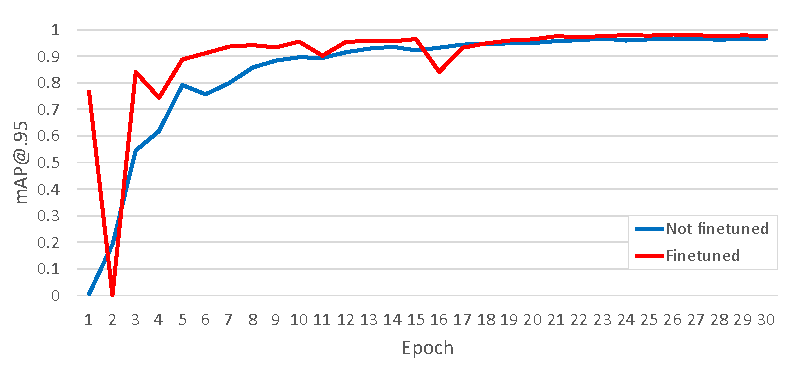
\includegraphics[width=1\textwidth]{img/design/nn-finetuned-vs-notfinetuned.pdf}
    \vspace{-20pt}
    \caption{A~comparison of~mAP@.95 development on~validation data during training a new model and finetuning an existing one proves that finetuning does not bring any benefit.}
    \label{nn-finetuned-vs-notfinetuned}
\end{figure}

Another argument selection concerns the batch size. Usually, a power of~2~is selected, namely one of~32~or~64. The YOLOv7 default is set to~16, so it was compared to~32~if it brings any improvements. Chart~\ref{nn-batch-16-vs-32} displays the difference. Lower batch sizes generally slow down the training as the weights are updated more often and the vectorization potential is reduced. Conversely, the more frequent weight updates might (not a rule) improve accuracy.

\vspace{-9pt}
\begin{figure}[!hbt]
    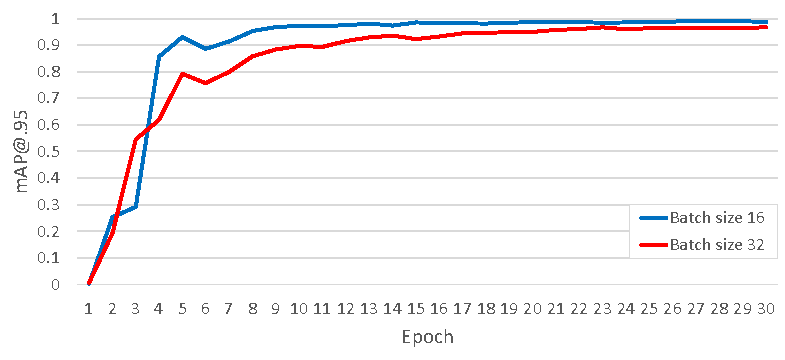
\includegraphics[width=1\textwidth]{img/design/nn-batch-16-vs-32.pdf}
    \vspace{-20pt}
    \caption{A~comparison of~mAP@.95 development on~validation data during trainings with batch sizes~16~and~32~clearly shows that batch size~16~achieves better results.}
    \label{nn-batch-16-vs-32}
\end{figure}

The remaining parameter, the number of epochs, was set to~30~for~visible reason in~both charts~\ref{nn-finetuned-vs-notfinetuned} and~\ref{nn-batch-16-vs-32}. Most of~the learning occurred in~the first~10~epochs, in~the next~10 there were significantly smaller improvements and in the last~10 it stabilized completely. In~this manner were trained all~3~640x640~models (yolov7-tiny, yolov7, yolov7-x) and the results are further discussed in~chapter~\ref{evaluation}. Full training results are available on~the attached medium~\ref{Appendix-A}.

Once the model is trained, the YOLOv7 project provides \emph{detect.py} script for the \hbox{actual} detection. However, this is not usable in~a custom solution. Therefore, Python pseudocode~\ref{yolov7-detect} demonstrates the model usage. Firstly, PyTorch loads the model and sets it from training to~evaluation mode. Secondly, the given image is transformed into~the detector's format, which means scaling and adding padding to~640x640 size and normalizing color values from~0-255~to~\hbox{0-1}. Then the model makes its predictions on which the non-maximum suppression method is applied. By~default, only the detections with a higher confidence score than~0.5~and only the best from the overlapping ones (iou = intersection over union threshold) are selected. Lastly, the detected bounding boxes are scaled back to the original image size.

\begin{algorithm}[!hbt]
    \begin{lstlisting}[keywords={def, return}, xleftmargin=20pt, numbers=left]
def detect(model_path, img, confidence=0.5, iou=0):
    model = torch.load(model_path)
    model.eval()
    input_img = prepare_img(img)
    predictions = model(input_img)
    predictions = non_maximum_suppresion(predictions, confidence, iou)
    predictions = scale_to_original(predictions, img)
        
    return predictions
    \end{lstlisting}
    \caption{Python pseudocode for a detection function using YOLOv7 model}
    \label{yolov7-detect}
\end{algorithm}

\section{Keys detection}
\label{design-keys}
Recognition of~keys on~a keyboard is the most challenging part of~this work. The Amazon research team used modified SSTD (Single Shot Text Detector)~\cite{sstd} architecture. SSTD serves for~text detection in~a scene image. However, it only finds text regions and does not recognize the text meaning~\cite{sstd}. The main modifications made were output change to~support multiple character classes and addition of~a non-maximum suppression layer so that it does not try to~join characters into~words~\cite{amazon-paper}. Nonetheless, I found~2~issues with~this approach. One of~them is that I do not see the point in~using a scene text detector and reducing its capabilities. Firstly, there is no real-world scene as~keyboards are basically just characters on~a background with some UI design. Secondly, the attention module for~text prediction in~SSTD misses the mark once the task is reduced to~single-character detection. The other problem is for~example the space key. In~many cases, the key is empty without any icon or \say{space} word. This leads~to a realization that just character recognition is not sufficient and a method for~the actual key (not its text) detection must be included. The proposed solution is to~use the current SOTA YOLOv7 for~the character recognition according to section~\ref{design-nn-chars} and Canny edge detector described by~section~\ref{design-classical-algorithms} for~checking the positions of those keys that have predefined locations such as~some special keys. This way there can be predicted potentially missing or incorrectly detected keys.

\subsection{Neural network design for character detection}
\label{design-nn-chars}
As~mentioned in~sections~\ref{algorithms-nn-yolo} and~\ref{design-keyboard}, YOLOv7 is the current SOTA in~object detection so it was selected for~this task as~well. Text detectors like SSTD or other OCRs usually aim at~detecting words or even sentences in~a scene. In~order to~achieve this, attention mechanism and other text-specialised methods are used~\cite{sstd}. This would make them more suitable models if text detection was the objective. Nevertheless, single-character detection is meant to~be solved. Consequently, the contextless feature of YOLOv7 is beneficial as it does not try to~merge the characters into~words.

The model was trained on~640x640 images from the generated dataset described in~section~\ref{dataset-characters}. To~fully disclose, there was no illusion of counting on great accuracy results, especially for~special characters such as dots, commas, semicolons etc. as~for~instance a semicolon can be recognized as~independent dot and comma. Many other examples like this one can be thought~of. A~lot of~such detection inaccuracies are solved by~the detection correction post-processing mechanism~\ref{design-keys-postprocessing}. Moreover, to~remind the task specification from section~\ref{introduction-expectation}, the main focus is on~alphanumeric characters. The endeavor to~recognize special characters as~well was made but as a secondary objective with a separate evaluation.

Concerning the actual training of~the model, it is the same as for~the keyboards described in~section~\ref{design-keyboard-implementation} with just~2~subtle differences. The first one is an increased number of~epochs to~50~as there are~99~classes and it takes longer to~train. The second one is a modification of~the original hyperparameters configuration file. Flipping of~objects during training was turned off because for example flipping the~left parenthesis results in~the right one which is a different class. Moreover, changes in~color, saturation and scale were reduced as it was already the subject of~dataset generation. The detector is further evaluated in~chapter~\ref{evaluation}.

When it comes to the usage of~the model to detect characters on~actual keyboards, an inconvenience comes up. Keyboards are usually very wide which is adversarial to the scaling. Let's assume a common scenario with a digital display where the keyboard covers about half of~the screen. On~the target full-HD image it would mean 1920x540 keyboard resolution which would scale down to 640x180. This results in~significant information loss and~2/3~of~the image under detection being padding. Instead of~simply scaling the image down, it is split and several detections are run. Full-HD width 1920px is convenient as it is exactly~3~times the width of~the detector's input. However, a certain overlap is necessary to avoid cutting a character in~half during the split. The overlap used is 64px which is the biggest font size on~which the model was trained. Consequently, the input image is split into several images which fit the 640x640 block. In~the case of the full-HD image with the overlap included, it is~4~images, but the algorithm is flexible so it is always split into the right number and no information is lost. The splitting is done only on the \emph{x}-axis, because 640px height is not expected to be exceeded or just slightly. Should it be significantly larger, the information loss during the scale-down is completely acceptable. Of~course, multiple detections influence negatively the performance. Nevertheless, the images can be batched and run in~a single computation just as another dimension of~the matrix. Furthermore, as YOLOv7 is a real-time detector with detection time in~milliseconds depending on~the machine, the slow-down is tolerable for~the use case.

\subsection{Key regions proposal using classical computer vision techniques}
\label{design-classical-algorithms}
The examples provided in~section~\ref{algorithms-classical} show that both edge detection and thresholding can produce satisfying results. Due to their similar results and no obvious reason why one should be better than the other, the Canny edge detection technique was chosen as the classical algorithm candidate because it is a bit simpler to use. The thresholding requires slightly more operations. Owing to~the simplicity and speed of this method, the initial idea was to use it as~a region proposer and then a classifier could be used to~recognize the characters. This strategy seemed to~solve it all. It could handle empty keys like space and achieve outstanding accuracy as~there already exist many character classifiers and datasets such as~MNIST. Despite~of~initial successes, though, two major issues concerning both edge detection and thresholding arose. The first one is contour computation depicted by~figure~\ref{canny-countour-problem}. As~there can be seen, many smaller regions were often detected instead of a full key. This might happen when an edge is not complete and has spaces in it which compromise the contour. Another complication is the detection of~both a key and a character. Which one to~use? The inner box (character) would be more suited for~the subsequent classification but then which to~choose e.g. between \emph{t} and~\emph{5}? It could be decided based on~the size but what if for~instance \emph{j} has its dot isolated or another contour error occurs? Too many inconvenient scenarios emerge which does not play well for~this strategy.

\begin{figure}[hbt]
    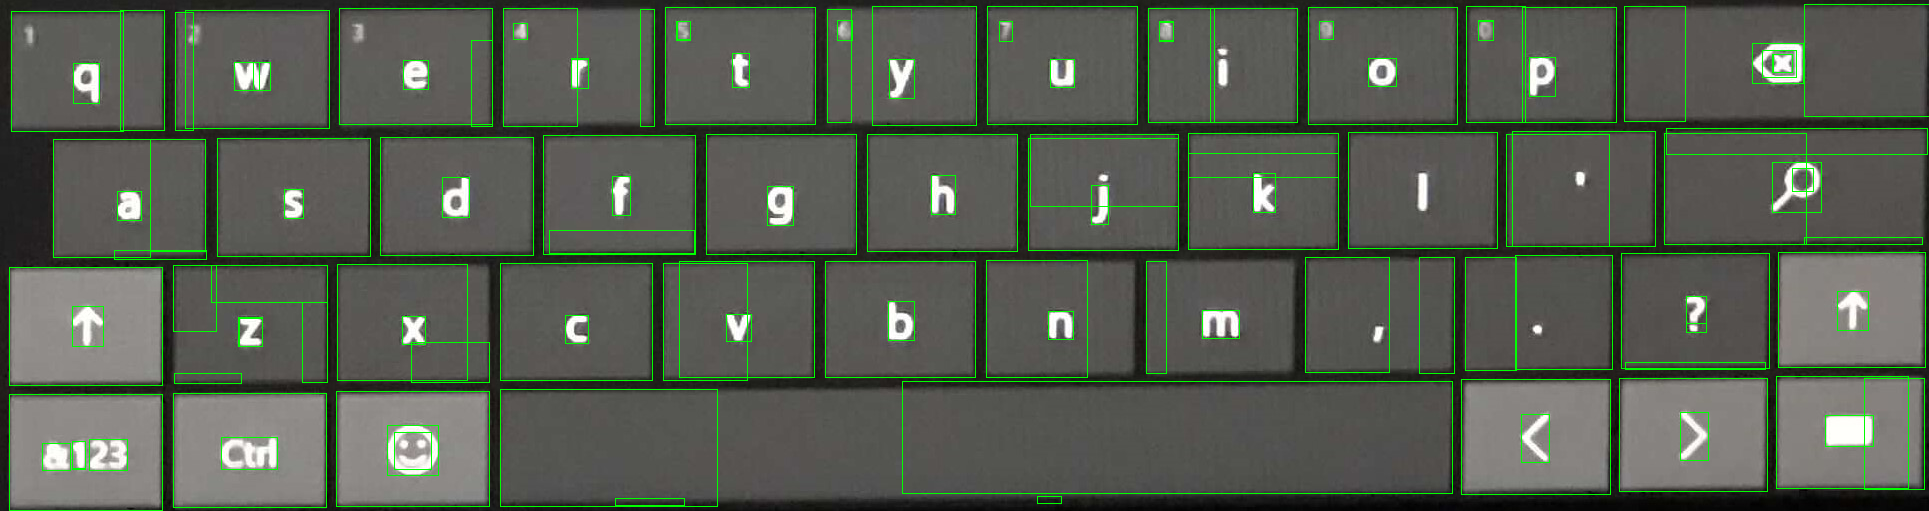
\includegraphics[width=1\textwidth]{img/design/canny-contour-problem.png}
    \caption{Contour computation problem in~edge detection region proposal}
    \label{canny-countour-problem}
\end{figure}

The second issue is the variety of UI designs that can create a huge amount of false positives. Something similar might happen with a background in a transparent keyboard. An example of such UI design is shown in~figure~\ref{canny-ui-problem}. Image (a) shows a car infotainment keyboard with vertical lines going to the background at~the bottom of the keyboard. This, however, renders the contour computation completely useless as~image (b) demonstrates. There would be a huge amount of~bounding boxes produced not only for the bottom vertical lines but also for the horizontal lines under the characters symbolizing the keys.

\begin{figure}[!tbh]
    \centering
    \subfloat[\centering Original image]{{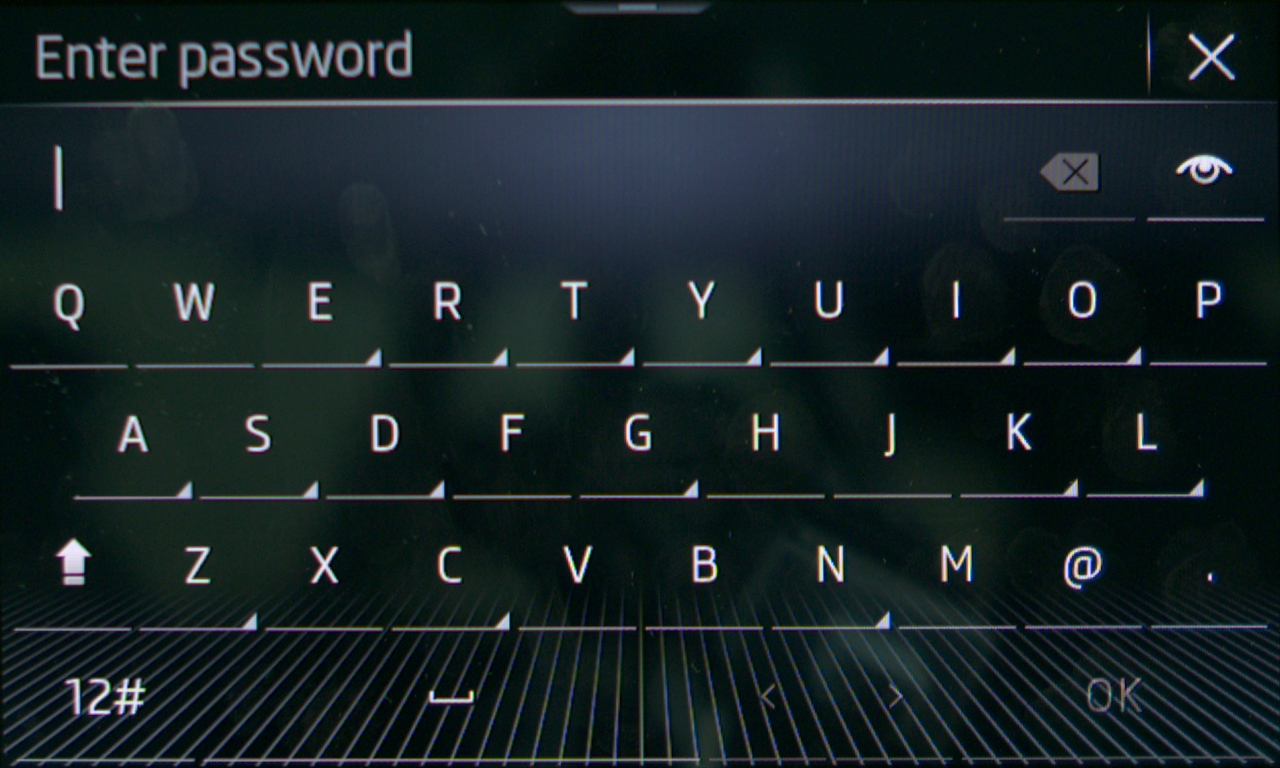
\includegraphics[width=7.45cm]{img/design/canny-ui-skoda-orig.jpg} }}
    \subfloat[\centering Binary image after Canny edge detection]{{\includegraphics[width=7.45cm]{img/design/canny-ui-skoda-binary.png} }}
    %\vspace{-6pt}
    \caption{UI keyboard designs can generate too many edges.}
    \label{canny-ui-problem}
\end{figure}

 What is more, it would be throwing out~the progress in~the object detection field and returning to~two-stage detectors. For these reasons, a detection neural network approach was opted for in~the end. Nevertheless, Canny edge detection is still run in~parallel as a supplementary bounding box provider of potential keys for the post-processing phase. Firstly, it costs almost nothing as it is computed parallelly. Secondly, the neural network does not solve the empty space key problem. If there is no icon or word on~the space key or it is not detected, the Canny edge detector might detect the key's rectangle. The same goes for other special keys such as shift if the icon or word is not detected. Which special keys are double-checked and how is the subject of section~\ref{postprocessing-canny}, the current section concentrates on~how the bounding boxes of~candidate key regions are obtained. The Python pseudocode~\ref{canny-pseudocode} describes the process.

\begin{algorithm}[!hbt]
    \begin{lstlisting}[keywords={def, return}, xleftmargin=20pt, numbers=left]
def run_canny_detection(img):
    img = clahe(img)
    img = cv2.cvtColor(img, cv2.COLOR_BGR2GRAY)
    img = cv2.bilateralFilter(img, 8, 30, 70)
    img = cv2.Canny(img, 25, 50)
    contours, _ = cv2.findContours(img)
    bboxes = convert_contours_to_bboxes(contours)

    return bboxes
    \end{lstlisting}
    \caption{Python pseudocode for Canny edge detection using OpenCV}
    \label{canny-pseudocode}
\end{algorithm}

Before the actual edge detection is performed, several image modifications to improve the detection results are done. To~highlight the edges a bit more, the clahe~\cite{clahe} contrast enhancing method is used. Then the image is transformed into a grayscale representation. Finally, bilateral filtering~\cite{opencv-library} is used to reduce noise while keeping edges. The second parameter~8~specifies the pixel neighborhood distance which influences the other parameters. The third one~30~is a relative measure of how much are the colors mixed together. The last parameter~70~is a relative measure of~how much the pixels influence each other taking the color into account as well. The subsequent Canny method accepts the lower and higher thresholds described in section~\ref{algorithms-classical-canny} and outputs a binary image with edges. Contours are computed for the edges and converted to~[x1, y1, x2, y2] bounding boxes.

\section{Post-processing of keys detection results}
\label{design-keys-postprocessing}
This is the third and final stage to~the whole process and it has several subtasks. In~general, it tries to validate the detected keys, correct any inaccuracies and fill in the undetected keys. For this purpose, supported layouts, keywords and other patterns are predefined as~rules and the detected characters are checked against these rules. To~make an example, let's assume we have a detected~\say{r} character and we want to check if it is the~\say{r} in~a qwerty row. The rule for this scenario says there should be \say{qwe} left of~the character and \say{tyuiop} right of~it. If there is a sufficient number of~matching characters in~the correct order, the check passes. Then the distances between characters are obtained and missing undetected characters can be computed or inaccurate bounding boxes corrected. Any sequence can be checked in~such a manner and the following sections describe each part in~more detail. The rule checking is the same, though. Before diving into the specifics, algorithm~\ref{postprocessing-algorithm} demonstrates the whole process.

\begin{algorithm}
    \hspace*{\algorithmicindent} \textbf{Input} Recognized characters \emph{chars} and Canny edge detection results \emph{canny\_bboxes} \\
    \hspace*{\algorithmicindent} \textbf{Output} Processed and accepted keys
    \begin{algorithmic}[1]
    \STATE $processed\gets \{\}$
    \STATE $rows\gets find\_rows(chars)$
    \STATE $check\_pinpad(rows, processed)$
    \STATE $check\_keywords(rows, processed)$
    \STATE $layout\gets check\_layout(rows, processed)$
    \STATE $check\_number\_line(rows, processed, layout)$
    \STATE $check\_icons(rows, processed, layout)$
    \STATE $check\_special\_characters(rows, processed, layout)$
    \STATE $guess\_special\_keys\_from\_canny(processed, canny\_bboxes, layout)$
    \STATE $correct\_capitalization(processed)$
    \end{algorithmic}
    \caption{High-level key detection post-processing process}
    \label{postprocessing-algorithm}
\end{algorithm}

In~the beginning, none of~the detected characters is accepted yet. Every detection is added to~the result only if it matches a rule. To have an idea about the detection placements and their relationships, they have to be organized into a structure. Simple rows were selected. For two bounding boxes to be in~the same row, they must overlap on~the \emph{y}-axis for at~least~50~\%. The rows are ordered bottom up and characters in~a row are ordered left to right by~the \emph{x}-axis. This is sufficient because keyboards are basically grids and it is easy to check a character's row for a sequence rule. Next, a pin-pad layout existence is checked. This is necessary to do before a layout recognition because otherwise the common alphabetical characters below or next to the pin-pad numbers could be incorrectly viewed as an alphabetical layout. Once it is clear whether a pin-pad keyboard is being processed or not, qwerty vs. alphabetical layout recognition can begin. Nevertheless, to reduce the number of~characters in~the layout recognition, keyword detection precedes it. Following is a 1-9 number line check, which is a very common sequence on~keyboards. Notice that zero is omitted as it can be either at~the start or end (more usual) of~the sequence. Then, special key icons and special characters are processed. These are basically the remaining detection results and with them ends any positional or correctional processing of~the character recognition. Thereafter, the Canny edge detection results are used to guess undetected special keys based on~the already detected ones. Finally, correction of~lower vs. upper case is performed. A~lot of characters such as x vs. X or s vs. S etc. are hardly distinguishable from each other and the character detector can easily make a mistake. For that reason, discrimi\-native characters \say{abdehmnqrty} whose lower and upper variants differ based on~intuition and character detector results are selected. All characters are set to the prevailing case among the discriminative characters. It is worth mentioning that at~the very beginning of~the post-processing, all characters are transformed to lowercase for easier manipulation and the information about their original case is saved for this part.

\subsection{Numbers processing}
\label{postprocessing-numbers}
There are~2~numbers-processing tasks performed. At~the very beginning of~the post-processing, a search for~a pin-pad layout is run. The \emph{x}~coordinates of~all numbers are checked against each other if they overlap to~find potential columns. The column patterns are 147, 258, and 369 so if for instance 4 overlaps with 7, it is considered a column. A third character is allowed to be missing to be computed. Then row patterns 123, 456, and 789 are searched for. If both a column and a row rules match, the pin-pad layout is recognized and any missing number is computed based on \emph{x} and \emph{y} differences in~found rows and columns. The method also counts with the possibility of both 123 and 789 rows being at~the top and at~the bottom of~the pin-pad. Nothing else is expected among the pin-pad characters, not even the usual alphabet characters as those are not keys, so every other detection inside the pin-pad layout can be removed. Finally, a zero is expected below the pin-pad so if any detected zero is positioned there, it is accepted as well.

The second task is the detection of~a number line \say{01234567890} where only one zero is expected but it can be on~either end. This takes place after the layout detection which is convenient. If it is a qwerty layout, it is expected for the number line to be above the top layout row. In~alphabetical layout or undetected layout (special characters mode or failed character recognition) it can be anywhere. Moreover, in~the second case, the line doesn't need to be full but cut and continued in~the next row. Therefore, the process is the following. Every detected and not yet accepted number is checked against the number line sequence rule. The check passes if there are at least~3~matches. In the case of a qwerty layout or full line acceptance, processing ends. Otherwise, the line could be cut and the action is repeated for the rest of~the numbers.

\subsection{Keywords processing}
\label{postprocessing-keywords}
The reason for keyword recognition is that the special keys might not have their icons but their names on~them. Furthermore, some special keys do not even have an icon. Because the keywords contain many characters which could negatively influence the layout recognition, the search for them happens before it and right after the pin-pad check. Moreover, the number of~characters to be processed in~layout recognition is reduced this way. Each special key can have several possible keywords and specific constraints. Generally, the requirement for~a minimum number of~matched characters in~a keyword for~a keyword rule to pass is~2/3 of its length. The target special keys are the following:

\begin{itemize}[topsep=0pt,itemsep=-1.5pt,partopsep=6pt]
  \item \textbf{Tab} --- This key has a single keyword \say{tab}. As it has a length of~3, two characters are sufficient for a match. However, due to \say{ab} being a very common sequence, the \say{t} needs to be one of~the recognized.
  \item \textbf{Caps Lock} --- Text on~this key is sometimes shortened to just \say{Caps} or \say{CapsLk}. Therefore, only the discriminative part \say{caps} is used for the keyword. Furthermore, detection of~\say{lock} can be misleading as it might be contained in~another key such as Num~Lock.
  \item \textbf{Shift} --- There is a single keyword \say{shift} for the key without any special treatment.
  \item \textbf{Space} --- A lot of~times, especially on~multilingual keyboards, the currently set language is written on~the space key. Hence, not only \say{space} but also \say{english} keywords are supported for~this key. In~addition, the \say{space} keyword is checked for~conflict with~\say{backspace} in~favor of~the latter.
  \item \textbf{Backspace} --- Apart from the \say{backspace} keyword, this key has two additional shortened variants \say{backsp} and \say{bksp} which both are supported.
  \item \textbf{Enter} --- Enter key supports \say{enter} and \say{return} keywords. The latter is especially common on~android devices.
  \item \textbf{Mode} --- This key is the most problematic one and supports many sequences which are commonly used for~the key such as \say{abc}, \say{123}, \say{?123}, \say{@\#\&}, \say{\#+=} and many others. The potential problems lie in~\say{abc} vs. alphabetical layout, \say{123} vs. pin-pad/number row or special character mode sequences vs. special characters on~a special character layout. Moreover, the \say{abc} usually means shift on~a character layout (qwerty, alphabet) and mode (switch to characters) on~a special character layout. Therefore, this keyword is saved for a retrospective classification based on~the detected layout and other detected keywords or icons. If there are other shift and mode keys recognized, it is ignored. Otherwise, it is the undetected one or a shift in~a character layout or a mode in~a special character layout.
  \item \textbf{Page} --- This is an edge case concerning special character modes. Sometimes, more than one page of~special characters is available, so this key searches for~\say{1/2} and \say{2/2} sequences with the slash character as a requirement.
\end{itemize}

Besides the sequence rules the distance between the characters must be checked. While in~a layout the characters are expected to have unknown spaces between them, keywords should have the characters in~close proximity. Therefore, if the characters are too far from each other where the tolerance is set to one-fifth of~the mean character width, the potential keyword is ignored. Similarly, if there are some undetected but expected characters and there is not enough space for~them, the candidate is not considered either.

When a candidate keyword passes all validations, it is not yet added to~the results but saved aside. The reason behind it are potential uninteresting words that might confuse the processing and cause mistakes. When a keyword is detected, it is saved only if it is the first of its kind or better than the already recognized one. Which one is better is determined by~the number of detected and skipped characters. As a consequence, only one special key of a kind is added to the accepted results. So if there are for example two shifts, which is common on~physical keyboards, one on~the left below Caps~Lock and one on the right below enter, only the more confident detection is used. On~one hand, a shift detection is lost, on~the other, it is absolutely of~no significance as~the key is detected and can be used.

\subsection{Layout processing}
\label{postprocessing-layout}
The goal of~this part is to~find an alphabetical or a qwert[y|z] layout among the detections. To~reduce the number of~processed characters and to~avoid errors as~much as~possible, only \hbox{layout} discriminative characters \say{dgkmquvwx} which are not part of~basic keywords (tab, caps, shift, space, enter) are used. Also, they are equally distributed by~3~in~each \hbox{qwerty} layout row.  Each of~the discriminative characters is checked against predefined \hbox{layout} rules. The rule sequence for alphabetical layout is \say{abc...xyz} where it is expected that it can be cut anywhere. The qwerty layout has sequences for each of~its rows (\hbox{\say{qwertyuiop}}, \hbox{\say{asdfghjkl}}, \hbox{\say{zxcvbnm}}) and any matched sequence suffices to~identify the layout. Undetected characters can be computed even in~other rows. The minimum matched \hbox{characters} requirement is only~2, so with~the currently processed character it makes~3~detected characters in~a row for the row to be considered as a layout row. This allows for a lot of~character detector mistakes which can be corrected but at~the same time more rows can be matched as the same sequence or one can match both layouts. Thus, all matches are saved as candidates and the best one is selected based on~the number of~detected and skipped characters. The winner's layout is set as~the recognized and is used as~a template for~missing characters computation. This is easy as~both \emph{x} and \emph{y} distances between characters are known from the detected ones.

In~the case of~a qwerty layout, additional processing can be done. Firstly, unmatched rows can be computed if at~least one character is detected in~them. This is not possible in~an alphabetical layout as it is unknown, where the row might be cut. Hence, the most confident detection of~each not yet accepted character is used but nothing else is computed. In~qwerty layout, on~the other hand, the rows are exactly defined, so the rest of~the row can be computed from a single detected character. Secondly, any other detections inside the qwerty layout are not allowed. Those can be either false positives or for example special characters foreshadowing their positions in~another mode as~figures~\ref{postprocessing-layout-qwerty-false-positives} and~\ref{postprocessing-layout-qwerty-removed-false-positives} depict.

\vspace{-4pt}
\begin{figure}[hbt]
    \includegraphics[width=1\textwidth]{img/design/postprocessing-layout-qwerty-false-positives.png}
    \vspace{-15pt}
    \caption{The detector can find characters in~a qwerty layout that are not keys.}
    \label{postprocessing-layout-qwerty-false-positives}
\end{figure}

\begin{figure}[!hbt]
    \includegraphics[width=1\textwidth]{img/design/postprocessing-layout-qwerty-removed-false-positives.png}
    \caption{Characters inside the qwerty layout are removed during the post-processing. The numbers above the top row are removed as well due to a margin added to the layout box for this very reason. Characters can be even horizontally outside as the right parenthesis in~the middle row demonstrates which is another reason for the margin.}
    \label{postprocessing-layout-qwerty-removed-false-positives}
\end{figure}

\subsection{Icons processing}
\label{postprocessing-icons}
Detected icons are processed after the layout and keywords are already known. This helps with icon validation and improves false positives detection. Generally, either a keyword or an icon is displayed on~a special key, so a recognized keyword might be an indication of~an invalid icon detection. Therefore, the keyword takes precedence and if it is detected, the icon is ignored. Also, the icon position is taken into~consideration relative to~the layout. Unfortunately, only the qwerty layout offers more or less standardized special key positions, so in~the case of~other layouts, simply the icons with~the highest detection confidence scores are used. The following describes the additional qwerty layout checks or other nuances for~each icon of~interest:

\begin{itemize}[topsep=0pt,itemsep=-1.5pt,partopsep=6pt]
  \item \textbf{Backspace} --- The key should be to~the right of~a qwerty layout so~it accepts the best only among such detections.
  \item \textbf{Enter} --- The check behaves exactly the same as for backspace.
  \item \textbf{Shift} --- The expected and preferred position is to~the left of~the \say{z} key. It might not necessarily be there, though. Next, it looks among those below \say{asd...} row. If not even there, the last check is anywhere to~the left of~the qwerty layout. It is not expected for~a shift to be anywhere else.
  \item \textbf{Tab} --- Tab is the most constraint special key. It is accepted only on~a qwerty layout and only in~its expected position which is left to~the \say{q} key. Thus, the rule of~keyword precedence works differently here. Retrospectively, the position of~the tab keyword is checked and it is removed if it is not correctly placed. This makes the icon the preferred choice, however, also only in~the right position.
  \item \textbf{Space} --- Similarly to~the tab key, the icon can take precedence if it is better positioned. Should the keyword be in~the bottom part of~the keyboard, any space icon is ignored. On~the contrary, the best icon is used with~the preference of~being below the bottom qwerty row.
\end{itemize}

\subsection{Special characters processing}
\label{postprocessing-special-chars}
There is only one pattern searched for among the special characters and it is !@\#\$\%\^{}\&*(). This sequence can be found above the qwerty layout or in~special character layouts. Other special characters are not part of~any rules and from those, only the most confident detection is used. Concerning the pattern, there exists a special case for qwerty layouts. Usually, the special characters above qwerty are on~the same keys as~numbers, where numbers are the main characters. For that reason, the existence of~a number line above the top qwerty row must be checked. If it is present, the special character line is ignored. Moreover, any special characters above the number line, special character line, or top qwerty row are removed as~those are considered the topmost keys in~qwerty layout keyboards.

\subsection{Canny detections processing}
\label{postprocessing-canny}
The objective is to find missing special keys. Unfortunately, too many unknowns limit this task. To~begin with, non-qwerty layouts tend to~have special keys anywhere so this action is constrained only to~qwerty layouts. Moreover, tab or caps~lock keys are not very common on~smartphones and generally on~touch screens, hence it is not even safe to assume their existence. Concerning enter and backspace, they should be present almost always and also the position ought to be to~the right of~the layout. However, their \emph{y}~position is the problem. The backspace key can be at~the top on~physical keyboards, at~the bottom on~smartphones, or even anywhere in~between depending on~the keyboard UI design. The same goes for~enter key which has the usual middle position but that is not a rule as~well. This leaves only shift and space keys. The space is one of~the main reasons for the edge detection as~it can be blank without any text or icon and there is no other way to~recognize it. In addition, it can be recognized quite easily as~it has its fixed position at~the bottom in~the middle and is significantly wider than all other keys. Then the shift key usually sticks to its position to~the left of~the bottom layout row. Furthermore, if it is not so, it is unlikely another key has its place. Thus, it can be relatively safely guessed that the found bounding box is indeed a shift. However, both space and shift key guessing occurs only if the corresponding key has not been found.

The input for this process are results of~the detection from section~\ref{design-classical-algorithms}. The accuracy might vary from very precise to~a lot of~noise bounding boxes which is the downside of~a method with fixed parameters. Therefore, filtration is necessary. As~the special keys are bigger than the character layout keys, the median size is computed and any smaller bounding box is removed. Furthermore, only bounding boxes from the bottom left quarter of~the image are considered as~neither of~the keys is expected to~be elsewhere. An example of~filtered bounding boxes is shown in~figure~\ref{demo-canny}. Once the filtration is complete, the bounding boxes matching the expected coordinates are selected as~the special keys.

\begin{figure}[hbt]
    \includegraphics[width=1\textwidth]{img/design/demo-canny.png}
    \caption{Canny detection targets shift and space keys which are constrained to~the bottom left quarter of~the image.}
    \label{demo-canny}
\end{figure}

\section{Final detection process}
\label{design-final-detection-process}
So far, individual parts of~the detection have been described. The whole process is summarized in~figure~\ref{detection-flow-chart}. The image processing starts with feeding the input image to~a trained YOLOv7 keyboard detection neural network model as outlined in~section~\ref{design-keyboard}. The output can be either used as a result of the required individual keyboard detection task or fed as input to~the subsequent character detection. On~the detected keyboard region is simultaneously run character detection using trained YOLOv7 model and Canny edge detection described in~sections~\ref{design-nn-chars} and~\ref{design-classical-algorithms}. The results of~these two detections are then processed in~the final post-processing phase presented in~section~\ref{design-keys-postprocessing}. The final results are bounding boxes with their confidence scores for recognized characters and keyboard in~JSON format. Optionally, images with rendered bounding boxes can be saved as well. The solution is very modular and it is easy to~switch or retrain a model if needed as~well~as include any additional post-processing. A~recognition running script is provided with the options of running full or partial (just keyboard or no post-processing) recognition.

\begin{figure}[hbt]
    \includegraphics[width=1\textwidth]{img/design/detection-flow-chart.png}
    \caption{Flow of the image recognition process}
    \label{detection-flow-chart}
\end{figure}

The image processing is also visually demonstrated by the following figures. As~an example is used one of~the images from the validation dataset. It illustrates changes done by~each recognition stage and also several post-processing corrections. The first step of~the process which is the keyboard region detection in~the input image is shown in~figure~\ref{demo-detection-keyboard}.

\begin{figure}[hbt]
    \includegraphics[width=1\textwidth]{img/design/demo-detection-keyboard.png}
    \caption{A keyboard region is detected in~the input image using the YOLOv7 model.}
    \label{demo-detection-keyboard}
\end{figure}

In~the next step, the detected keyboard region is used as~input for the detection of~keys. Figure~\ref{demo-detection-chars} depicts single-character detection results. This detection is run in~parallel with the Canny edge detection described in~section~\ref{postprocessing-canny}. As~can be seen, the detector made some mistakes. It did not recognize characters \hbox{e, i, a, s, l} and has false positive detections for~tab and~Q character at~the bottom right corner. In~addition, it incorrectly classified o~as~0. Other than that, the detections are accurate. There can also be noticed sequence ?123 which stands for a~keyboard mode changing key. It is up to the post-processing algorithm to find it.

\begin{figure}[!hbt]
    \includegraphics[width=1\textwidth]{img/design/demo-detection-chars.png}
    \caption{Individual characters are detected in~the keyboard using the YOLOv7 model.}
    \label{demo-detection-chars}
\end{figure}

Next, figures~\ref{demo-postprocessing} and~\ref{demo-full-postprocessing} show the post-processing phase. In~figure~\ref{demo-postprocessing} the algorithm computed the missing characters (cyan bounding boxes) and also managed to correct \hbox{the o vs. 0} mistake. Moreover, no rule for the false positive tab and Q was matched so they were removed. Furthermore, the~mode sequence was found and converted to a new key bounding box.

\begin{figure}[hbt]
    \includegraphics[width=1\textwidth]{img/design/demo-postprocessing.png}
    \caption{Character detections are corrected and missing characters are computed in~the post-processing phase.}
    \label{demo-postprocessing}
\end{figure}

In~figure~\ref{demo-full-postprocessing} can be seen the final post-processing result including the Canny detections. It differs from the figure~\ref{demo-postprocessing} in~that it has the space key recognized. Moreover, the computed keys are not visually distinguished.

\begin{figure}[!hbt]
    \includegraphics[width=1\textwidth]{img/design/demo-full-postprocessing.png}
    \caption{The post-processing is completed by~incorporating the Canny detection results, namely the space key.}
    \label{demo-full-postprocessing}
\end{figure}

As~already mentioned, the example image comes from the validation dataset. Therefore, to~visually show the recognition accuracy, figure~\ref{demo-evaluation} illustrates the detected and expected keys. The green bounding boxes are the detected ones while the yellow show the expected coordinates. Almost all characters/keys were recognized and the overlap with the ground truth is very good. However, there can be noticed two undetected magenta bounding boxes for~dot and comma characters. Finally, after transforming the detections back to~the original image, figure~\ref{demo-full-detection} depicts the complete keyboard recognition result.

\begin{figure}[!hbt]
    \includegraphics[width=1\textwidth]{img/design/demo-evaluation.png}
    \caption{The detected keys (green) match very well the expected ones (yellow).}
    \label{demo-evaluation}
\end{figure}

\begin{figure}[!hbt]
    \includegraphics[width=1\textwidth]{img/design/demo-full-detection.png}
    \caption{Fully processed image as~a result of~the image recognition}
    \label{demo-full-detection}
\end{figure}

  \chapter{Evaluation of results}
\label{evaluation}
In~this chapter, individual recognition phases are evaluated. Some evaluation of~YOLOv7 training strategies was already done in~section~\ref{design-keyboard-implementation}. There were discussed differences between~16~vs.~32~batch size and finetuning vs. new training. Furthermore,~three~versions of~640x640~YOLOv7 models were introduced. The following sections~\ref{evaluation-keyboard} and~\ref{evaluation-chars} present the comparison of the YOLOv7 variations (yolov7-tiny, yolov7, yolov7-x) and discuss the choices made. The last section~\ref{evaluation-postprocessing} shows results of~the post-processing algorithm on~its validation dataset. The metrics used for the evaluation are precision, recall and for~the YOLOv7 models also mAP. The mAP was computed for~0.5 and~0.95 intersection-over-union values. A~full account of~the results is available on~the attached medium~\ref{Appendix-A}, here only selected metrics and results are used for~demonstration.

\section{Keyboard detector}
\label{evaluation-keyboard}
As~described in~section~\ref{design-keyboard-implementation}, yolov7-tiny is smaller, faster and uses fewer resources than the original YOLOv7 variation from the paper~\cite{yolov7} at~the cost of~accuracy. On~the contrary, yolov7-x is supposed to~be more accurate at~the cost of~reduced processing speed, higher resource consumption and bigger size. Figure~\ref{eval-keyboard-resources} illustrates the comparison in~resource consumption on~averaged memory allocation in~percents on~a \hbox{2-core} GPU provided by~Kaggle platform. The relative difference between the models is very similar in~GPU utilization and other physical metrics as well. Another factor is the actual size of~the models. The tiny model has only about~12~KB, while the original one takes about~73~KB and the yolov7-x even~140~KB. So~far, the tiny version is the winner. The comparison of~mAP@.95 metric development during the training, which gives an account of~the accuracy properties of~the models, is shown in~figure~\ref{eval-keyboard-training}. Recall, precision and loss functions are available on~the attached medium~\ref{Appendix-A}, but as~mAP is dependent upon recall and precision, it is a sufficient representation of~the detector's overall capabilities. As~can be seen, the training progressed very similarly and all 3~models came to the same results. This proves that for the keyboard detection task, the bigger models do not bring any additional value. Hence, the yolov7-tiny version is used as it is as accurate as the other versions while being significantly faster and requiring fewer computational resources. The full account of~the training results on~the testing dataset is in~table~\ref{eval-table-keyboard}. Apart from mAP@.95 the results are identical. There can be seen a slight improvement in~mAP@.95 among the bigger models, but that can be viewed as~insignificant. The~near~2~\% difference between yolov7-tiny and yolov7-x is negligible especially if taking into consideration the cost of~size, speed and resources.

\begin{figure}[hbt]
    \includegraphics[width=1\textwidth]{img/evaluation/eval-keyboard-resources.pdf}
    \caption{The tiny version of~the YOLOv7 proves to be substantially more efficient in~terms of~resource consumption. Comparisons of~other physical metrics look fairly similar.}
    \label{eval-keyboard-resources}
\end{figure}

\begin{figure}[!hbt]
    \includegraphics[width=1\textwidth]{img/evaluation/eval-keyboard-training.pdf}
    \caption{The development of~mAP@.95 on~validation data during training indicates a minimal difference in~the expressive power of~the models.}
    \label{eval-keyboard-training}
\end{figure}

\vspace{12pt}
\begin{table}[!hbt]
\begin{tabular}{
|p{0.2\textwidth}|>{\centering\arraybackslash}p{0.164\textwidth}|>{\centering\arraybackslash}p{0.164\textwidth}|>
{\centering\arraybackslash}p{0.164\textwidth}|>
{\centering\arraybackslash}p{0.164\textwidth}|}
 \hline
 \centering Model & Precision & Recall & mAP@.5 & mAP@.95\\
 \hline
 yolov7-tiny & 1 & 1 & 0.996 & 0.971 \\
 yolov7 & 1 & 1 & 0.997 & 0.98 \\
 yolov7-x & 1 & 1 & 0.997 & 0.989 \\
 \hline
\end{tabular}
\caption{The results of~individual models on~the testing keyboard dataset show that all of~them are almost equally accurate.}
\label{eval-table-keyboard}
\end{table}

\section{Character detector}
\label{evaluation-chars}
Due to using the same model as for the keyboard detection, the character detector was evaluated in~the same manner. Concerning resource consumption, the difference between the models got reduced as~can be seen in~figure~\ref{eval-char-resources}. The tiny model is still the clear winner, but not as~notably as~in~keyboard detection shown in~figure~\ref{eval-keyboard-resources}. This is caused by~the increased number of~classes and thus a greater number of~detections made.

\begin{figure}[hbt]
    \includegraphics[width=1\textwidth]{img/evaluation/eval-char-resources.pdf}
    \caption{The resource consumption is a bit more leveled than in~keyboard detection, but the fact that the bigger the model the higher the consumption still holds. Again, other metrics such as~GPU utilization show similar differences.}
    \label{eval-char-resources}
\end{figure}

When it comes to~the expressive power of~the models, the tiny model falls behind as~demonstrated by~figure~\ref{eval-char-training}. The bigger models are again almost identical, with the difference that yolov7-x was trained slightly smoother. The higher number of~classes and presumably some similar-looking characters are problematic for the tiny model though. Nevertheless, it is still quite sure with itself as~figure~\ref{eval-char-training-precision} shows. While it still cannot reach the same precision as~the bigger models and it climbs slower, it eventually comes close. The problem lies in~recall where the chart looks similar to~figure~\ref{eval-char-training}. It simply cannot detect as~many characters and the ones detected have lower confidence scores. The complete results are laid out in~table~\ref{eval-table-chars}. The yolov7-x version again does not bring any improvement so due to its size it is considered no more. Thus, the original YOLOv7 model is selected for~the character recognition task. However, the next section~\ref{evaluation-postprocessing} explains why the tiny model might still be of~use. The presented data are overall results. Character-specific metrics are available on~the attached medium~\ref{Appendix-A}. To demonstrate the accuracy variability of~individual characters, figure~\ref{eval-char-f1} shows their F1 curves. The lowest curves belong to special characters such as~dot, comma or underscore while the top ones are for special key icons and capital alphabet characters. In~conclusion, it is visible that the accuracy varies which was expected not only because of~special characters but also non-discriminative upper and lower case letters.

\begin{figure}[hbt]
    \includegraphics[width=1\textwidth]{img/evaluation/eval-char-training.pdf}
    \caption{The development of~mAP@.95 on~validation data during training indicates that bigger yolov7-x is not stronger that the normal version. However, in~comparison with the keyboard detector, the tiny version is not as~accurate~as the bigger models.}
    \label{eval-char-training}
\end{figure}

\vspace{12pt}
\begin{figure}[!hbt]
    \includegraphics[width=1\textwidth]{img/evaluation/eval-char-training-precision.pdf}
    \caption{The development of~precision on~validation data during training shows that the bigger models have the same precision. The tiny version falls behind a bit but it is still competitive.}
    \label{eval-char-training-precision}
\end{figure}

\begin{table}[!hbt]
\begin{tabular}{
|p{0.2\textwidth}|>{\centering\arraybackslash}p{0.164\textwidth}|>{\centering\arraybackslash}p{0.164\textwidth}|>
{\centering\arraybackslash}p{0.164\textwidth}|>
{\centering\arraybackslash}p{0.164\textwidth}|}
 \hline
 \centering Model & Precision & Recall & mAP@.5 & mAP@.95\\
 \hline
 yolov7-tiny & 0.948 & 0.852 & 0.912 & 0.748 \\
 yolov7 & 0.979 & 0.951 & 0.977 & 0.848 \\
 yolov7-x & 0.98 & 0.95 & 0.978 & 0.858 \\
 \hline
\end{tabular}
\caption{The results of~individual models on~the testing character dataset show that while the tiny model is less accurate, especially in~terms of~recall and mAP@.95, the difference between the normal and bigger versions is minuscule.}
\label{eval-table-chars}
\end{table}

\begin{figure}[hbt]
    \includegraphics[width=0.95\textwidth]{img/evaluation/eval-char-f1.png}
    \caption{The majority of F1 curves for individual characters (gray) is better than the overall F1 curve (blue) from the original YOLOv7 model on~character testing dataset. This is due to some less accurate special characters.}
    \label{eval-char-f1}
\end{figure}

\section{Post-processing algorithm}
\label{evaluation-postprocessing}
The character detector's results show that there is room for~improvement. The post-processing algorithm not only improves overall recognition results but also removes the accuracy gap between the tiny and normal models. On~the post-processing validation dataset, the character recognition with applied post-processing achieves similar though slightly worse results shown in~table~\ref{eval-postprocessing-table} than the single-character detection on~the \hbox{character} dataset. Notwithstanding, the results are still impressive considering this is a real-world and not a~generated dataset. Moreover, these are averaged numbers impaired with special character detection on which not much post-processing is done.

As~the table shows, the results for special characters are nowhere near as good as for the other keys. Partially, it is due to dots~vs.~noise/commas/colons/semicolons or underscores~vs.~dashes etc. It may to a degree be also due to some low-quality validation images. As~not many full-HD samples could be obtained, the dataset consists of~keyboards of~diverse quality. It can be presumed that on~full-HD images from~AIVA cameras, the results might be slightly better. It is worth reminding, that special character recognition was not the main objective so~for a bonus the results can still be considered satisfactory.

The special keys results are significantly better. Though they are not yet perfect, \hbox{taking} into account that these keys do not have to have just icons but also words on~them, the results are favorable. The letters in~words are usually much smaller than on~regular keys, hence harder to recognize. Furthermore, because of~the close proximity to~other characters in~the word, the detector can be easily baffled, especially in~lower-quality images. Consequently, joining letters to~words and recognizing the words in~spite of~missing (undetected or incorrectly detected) letters with such precision and recall is considered a success.

Despite special characters not doing so well, the results for target alphanumeric characters exceed expectations and show how powerful the post-processing really is. The reason for this is quite simple. Let's consider a qwerty layout. All the detector needs to recognize is one character in~each row and at~least a minimum-requirement number of~characters in~a row for the layout to~be recognized as~qwerty. This gives the algorithm a starting point and both \emph{x} and \emph{y} distances between characters. The rest can be computed or corrected with almost~100~\%~accuracy. As~a~consequence, the detector's responsibility is to provide just a bare minimum. This is also the reason why the tiny model actually performs slightly better. It does not produce as~many false positives to~confuse the algorithm as~the normal version does and the undetected characters can be easily computed.

\begin{table}[hbt]
\begin{tabular}{
|p{0.2\textwidth}|>{\centering\arraybackslash}p{0.164\textwidth}|>{\centering\arraybackslash}p{0.164\textwidth}|>
{\centering\arraybackslash}p{0.164\textwidth}|>
{\centering\arraybackslash}p{0.164\textwidth}|}
\hline
& \multicolumn{2}{c|}{yolov7} & \multicolumn{2}{c|}{yolov7-tiny}\\
 \hline
 & Precision & Recall & Precision & Recall\\
 \hline
 All keys & 0.942 & 0.949 & 0.964 & 0.942\\
 Alphabet & 1 & 1 & 1 & 1\\
 Numbers & 0.998 & 0.987 & 1 & 0.993\\
 \textbf{Alphanumeric} & \textbf{0.999} & \textbf{0.997} & \textbf{1} & \textbf{0.998}\\
 Special keys & 0.965 & 0.910 & 0.987 & 0.914\\
 Special characters & 0.684 & 0.767 & 0.762 & 0.705\\
 \hline
\end{tabular}
\caption{Among the results of~the post-processing algorithm on~the validation dataset stand out alphanumeric characters.}
\label{eval-postprocessing-table}
\end{table}
  \chapter{Conclusion}
\label{conclusion}

In~this work, a research was done into~popular object detection methods and a summary was made. Special attention was paid to~the evolution of~YOLO algorithm where each version until the most recent one at the time of writing the thesis was described. Particular detail was given to the current state-of-the-art YOLOv7. Moreover, datasets for~keyboard detection, single-character detection and post-processing were devised and created. These datasets were used for~training and validation of~the recognition methods. The datasets are unique as~no other is to~the best of~my knowledge publicly available. They can serve not only the~keyboard typing automation task but also any other which might use keyboard detection or single-character detection. Then, a three-phased image processing strategy was designed and implemented. Firstly, YOLOv7 neural network model is used for~keyboard detection. Secondly, characters are recognized in~the detected keyboard region again using YOLOv7. The found characters symbolize potential keys and are further processed in~the last stage. The post-processing algorithm corrects mistakes based on~predefined supported layouts. Furthermore, it can be easily extended to~handle new scenarios. The results of~each phase were evaluated and found satisfactory. The accuracy of the methods exceeds expectations, particularly keyboard detection and recognition of~alphanumeric characters. Consequently, a novel modular solution for~keyboard and keys recognition was created which can be effortlessly extended or its parts replaced. This solution is to~be used in~the production environment of~Y~Soft~AIVA system where it will help with automating robotic keyboard typing. On~top of~that, the thesis received Jiří Kunovský award from Excel@FIT~2023 conference based on~votes from the professional public.

In~future work, the actual integration into~the AIVA system needs to~be done. Other than that, there is room for~improvement with respect to~special characters' accuracy. Moreover, additional character sets can be supported such as other alphabets, diacritics or more \hbox{special} characters. The same holds for~support of~new keyboard layouts. Also, as~new state-of-the-art detectors will be emerging, the models can get retrained to~improve the overall results.




  
  % Kompilace po částech (viz výše, nutno odkomentovat)
  % Compilation piecewise (see above, it is necessary to uncomment it)
  %\subfile{projekt-01-uvod-introduction}
  % ...
  %\subfile{chapters/projekt-05-conclusion}


  % Pouzita literatura / Bibliography
  % ----------------------------------------------
\ifslovak
  \makeatletter
  \def\@openbib@code{\addcontentsline{toc}{chapter}{Literatúra}}
  \makeatother
  \bibliographystyle{bib-styles/Pysny/skplain}
\else
  \ifczech
    \makeatletter
    \def\@openbib@code{\addcontentsline{toc}{chapter}{Literatura}}
    \makeatother
    \bibliographystyle{bib-styles/Pysny/czplain}
  \else 
    \makeatletter
    \def\@openbib@code{\addcontentsline{toc}{chapter}{Bibliography}}
    \makeatother
    \bibliographystyle{bib-styles/Pysny/enplain}
  %  \bibliographystyle{alpha}
  \fi
\fi
  \begin{flushleft}
  \bibliography{Bibliography}
  \end{flushleft}

  % vynechani stranky v oboustrannem rezimu
  % Skip the page in the two-sided mode
  \iftwoside
    \cleardoublepage
  \fi

  % Prilohy / Appendices
  % ---------------------------------------------
  \appendix
\ifczech
  \renewcommand{\appendixpagename}{Přílohy}
  \renewcommand{\appendixtocname}{Přílohy}
  \renewcommand{\appendixname}{Příloha}
\fi
\ifslovak
  \renewcommand{\appendixpagename}{Prílohy}
  \renewcommand{\appendixtocname}{Prílohy}
  \renewcommand{\appendixname}{Príloha}
\fi
%  \appendixpage

% vynechani stranky v oboustrannem rezimu
% Skip the page in the two-sided mode
%\iftwoside
%  \cleardoublepage
%\fi
  
\ifslovak
%  \section*{Zoznam príloh}
%  \addcontentsline{toc}{section}{Zoznam príloh}
\else
  \ifczech
%    \section*{Seznam příloh}
%    \addcontentsline{toc}{section}{Seznam příloh}
  \else
%    \section*{List of Appendices}
%    \addcontentsline{toc}{section}{List of Appendices}
  \fi
\fi
  \startcontents[chapters]
  \setlength{\parskip}{0pt} 
  % seznam příloh / list of appendices
  % \printcontents[chapters]{l}{0}{\setcounter{tocdepth}{2}}
  
  \ifODSAZ
    \setlength{\parskip}{0.5\bigskipamount}
  \else
    \setlength{\parskip}{0pt}
  \fi
  
  % vynechani stranky v oboustrannem rezimu
  \iftwoside
    \cleardoublepage
  \fi
  
  % Přílohy / Appendices
  \chapter{Contents of the attached medium}
\label{Appendix-A}

\begin{itemize}
  \item \texttt{/doc} --- Solution documentation
    \begin{itemize}
        \item \texttt{/latex} --- LaTex source code for the thesis
        \item \texttt{thesis.pdf} --- This text of the thesis
    \end{itemize}
  \item \texttt{/results} --- Image processing results
    \begin{itemize}
        \item \texttt{/models} --- Trained models for keyboard and character detection
        \item \texttt{/statistics} --- Numeric and visual training and evaluation results
        \item \texttt{training\_metrics.xlsx} --- Metrics for each training
    \end{itemize}
  \item \texttt{/src} --- Source code of the solution
\end{itemize}

\chapter{Excel@FIT 2023 Poster}
\includepdf[pages=-,offset=0.7cm -1.46cm]{img/excel_fit_poster.pdf}

\chapter{Excel@FIT 2023 Article}
\includepdf[pages=-,offset=0.7cm -1.46cm]{img/excel_fit_article.pdf}

  
  % Kompilace po částech (viz výše, nutno odkomentovat)
  % Compilation piecewise (see above, it is necessary to uncomment it)
  %\subfile{projekt-30-prilohy-appendices}
  
\end{document}
